\PassOptionsToPackage{table, dvipsnames}{xcolor}
\documentclass[11pt]{beamer} %%

%%% option passed to the outer theme
% fixedCircCnt,   % (moving is deault)
\usetheme[progressstyle= movingCircCnt]{Feather}


%%xcolor=dvipsnames,
%-------------------------------------------------------
% INCLUDE PACKAGES
%-------------------------------------------------------

\usepackage[utf8]{inputenc} 
\usepackage{graphicx}
\usepackage{tikz}
\usetikzlibrary{decorations.fractals}
\usepackage{wrapfig}
\usepackage[english]{babel}
\usepackage{amsmath}
\usepackage{braket}
\usepackage{wrapfig}
\usepackage{mathpazo} 
%\usepackage{amssymb}
\usepackage{amsmath, amsthm, amssymb}

\usepackage{amsfonts}
%\usepackage{mathrsfs}
\usepackage{slashed} % Dirac slash
\usepackage{pifont}
\usepackage{caption}

%%%% multimedia
%%\usepackage{multimedia}
%%\usepackage{hyperref}


%%%% fonts
\usepackage{tgtermes}
%% change font of the document 
%\renewcommand*{\familydefault }{\mrdefault}
\usefonttheme{professionalfonts} % using non standard fonts for beamer
\usefonttheme{serif} % default family is serif
\usepackage{fontspec}
\setmainfont{Latin Modern Roman}

%%%% colors
% Change the frame title text color:
\setbeamercolor{frametitle}{fg=BurntOrange}
% Change the normal text color background:
\setbeamercolor{normal text}{fg=black,bg=white}
%%% color equations 
\usepackage[skins,theorems]{tcolorbox}
\tcbset{highlight math style={enhanced,
  colframe=red,colback=white,arc=0pt,boxrule=1pt}}

%%%% colourful equation box
\tcbset{highlight math style={enhanced,
  colframe=red,colback=white,arc=0pt,boxrule=1pt}}
\newcommand{\eqbox}[3]
           {
             \tcbhighmath[boxrule=2pt,arc=1pt,colback=#1!10!white,colframe=#2!40,
               drop fuzzy shadow=white] {#3}
           }

%%%%  tables
%%\usepackage[landscape]{geometry}
\usepackage{multirow}
\usepackage{changepage}
\usepackage{longtable}
\usepackage{booktabs}

%% for pdf input
\usepackage{pdfpages}

\usepackage{forloop}

%%%% set footers
\setbeamertemplate{footline}[text line]{%
  \parbox{0.3\linewidth}{\vspace*{-5pt}\hspace*{0.5cm}
    \textcolor{BurntOrange}{{-- Neutrino Detectors}}}\hfill
  \parbox{0.4\linewidth}{\vspace*{-5pt}\hspace*{1.cm}
    \textcolor{BurntOrange}{{ -- Sina Bahrasemani --}}}\hfill
  \parbox{0.3\linewidth}{\vspace*{-5pt}\hspace*{1.5cm}
    \textcolor{BurntOrange}{{Fall 2017 --}}}\hfill
}
%%\setbeamertemplate{footline}[page number]

% colored hyperlinks
\newcommand{\chref}[2]
           {
             \href{#1}{{\usebeamercolor[bg]{Feather}#2}}
           }

%%%% few extra commands
\renewcommand{\(}{\begin{columns}}
\renewcommand{\)}{\end{columns}}
\newcommand{\<}[1]{\begin{column}{#1}}
\renewcommand{\>}{\end{column}}

\newcommand{\itt}{\begin{itemize}}
\newcommand{\tti}{\end{itemize}}

\newcommand{\img}[1]{\includegraphics[width=\linewidth]{./Images/#1}}

\newcommand{\hlt}[2]{\textcolor{#1}{\textbf{#2}}}
\newcommand{\ntit}[1]{\qquad\qquad\qquad\qquad\hlt{blue}{\Large #1}\\~\\}
%% \newcommand{\hlt1}[1]{\textcolor{Goldenrod}{\textbf{#1}}}
\newcommand{\cmark}{\ding{51}}%
\newcommand{\done}
           {
             \rlap{$\square$}
                  {\raisebox{2pt}
                    {
                      \large\hspace{0.1pt}
                      \textcolor{green}{\cmark}
                    }
                  }
                  \hspace{-2.5pt}
           }

           
%%% counting backup slides
\newcommand{\beginbackup}
           {
             \newcounter{framenumbervorappendix}
             \setcounter{framenumbervorappendix}{\value{framenumber}}
           }
\newcommand{\backupend}
           {
             \addtocounter{framenumbervorappendix}{-\value{framenumber}}
             \addtocounter{framenumber}{\value{framenumbervorappendix}} 
           }

%%%% Loading packages DONE!
%\logo{
\includegraphics[scale = 0.2]{./Images/SFU_logo.jpg}}

\begin{document}
%%%% SLIDE 1: title page
\begin{frame}
	\vspace{0.9cm}

\title[]{Neutrino Detectors}
\author{Sina Bahrasemani\\
  \vspace{0.2in}
}
\date{
  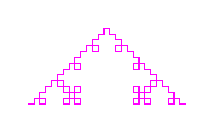
\begin{tikzpicture}[decoration=Koch curve type 1] 
    \draw[Magenta] decorate{ decorate{ decorate{ (0,0) -- (2,0) }}}; 
  \end{tikzpicture}  
  \\
  \vspace{0.2cm}
  \today
}
\titlepage
\end{frame}

%%%%%%%% SLIDE 2: outline page
\begin{frame}{Outline}
\small
\tableofcontents
\end{frame}


%% cite An Introduction to Cherenkov Radiation, Hadiseh	Alaeian
%%%% SLIDE 4
% %\subsection{Cherenkov Radiation}
% \begin{frame}{\textcolor{Goldenrod}{Cherenkov Radiation}}
%   \(
%   \<{0.35\textwidth}
%   \img{cherenkov_rad}
%   \>
%   \<{0.75\textwidth}
%   \hlt{LimeGreen}{When a charged particle moves
%     inside a medium it excites the atoms and molecules of the
%     matter and they emit radiation.}
%   \[
%     \alert{\cos{\theta_{p, \gamma}} = \frac{1}{n \beta } +
%       \frac{(n^2 -1)h\nu}{2P_i c n}}
%   \]
%  \itt
% \item[$\Box$] \hlt{Red}{There's no emission below a threshold velocity
%     $\beta_t = \frac{1}{n}$}.
% \item if the refractive index of a materials drops below 1, no
%   Cherenkov radiation can be observed within that range.
%   \tti
%   \>
%   \)
% \end{frame}

% %%%%%%%%%% SLIDE 
% \begin{frame}{\textcolor{Goldenrod}{Cherenkov Radiation Spectrum}}
%   \hlt{Blue}{The number of radiation emitted $dE$ per unit length $dx$ per unit
%     frequency $d\omega $ is  given by the Frank-Tamm formula:}
%   \[
%     \begin{aligned}
%       &\textcolor{Magenta}{\frac{dE}{dx} = 2 \pi^2 r_e mc^2 \sin^2\theta
%         [\frac{1}{\lambda^2_i} - \frac{1}{\lambda^2_f}]}\\
%       &\textcolor{Green}{\frac{dN}{dx} = 2 \pi^2 \alpha \sin^2\theta
%         [\frac{1}{\lambda_i} - \frac{1}{\lambda_f}]}
%     \end{aligned}
%   \]
%   \itt
% \item \textcolor{blue}{The emitted energy is peaked at short wavelengths(blue light)}
% \item Cherenkov radiation is smaller than energy loss due to
%   ionization $2 MeV/cm$ and scintillation. 
%   \tti
% \end{frame}

% %%%%%%%%% SLIDE
% \begin{frame}{\textcolor{Goldenrod}{Cherenkov Counters}}
%   \itt
% \item[$\Box$] Threshold: detects particles over a velocity range $ [1/n,
%   1/\sqrt{n^2 -1}]$
%   \itt
% \item The detection efficiency of a threshold counter increases rapidly as the
%   velocity of the incident particles.
%   \tti
% \item[$\Box$] Differential: {can measure the velocity of a particle
%     by only accepting Cerenkov light in a small annulus around some angle
%     $\theta$.}
%   \itt
% \item only accepts light from within the angular range
%   $
%   \Delta \theta = \cos^2\theta \frac{\Delta r}{f}
%   $
%   \tti
% \item[$\Box$] Ring Imaging (RICH):
%   The radiating medium is contained
%   between two spheres surrounding the target or intersection point.
%   \itt
% \item The Cerenkov light reflects off the mirror and is focused onto a ring at
%   the detector surface.
%   \[
%     \beta = \frac{1}{\cos(2r/R_s)}
%   \]
%   \tti
%   \tti
% \end{frame}

% %%%%%%%% TRD , TRT
% \begin{frame}{\textcolor{Goldenrod}{Transition Radiation }}
%   \hlt{Blue}{Transition Radiation (TR) happens when a charged particle moves through
%     an inhomogeneous media (different dielectric constants)}
%   \itt
% \item The energy spectrum radiated by a charged particle with a Lorentz factor
%   $\gamma$ traversing an interface between two dielectric media (with
%   dielectric constants $\epsilon_1$ and $\epsilon_2$) is as following:
%   \[
%     \frac{dE}{d\nu d\Omega} =  \frac{\alpha^2}{\pi^2}
%     (\frac{\theta}{\gamma^{-2}+\theta^2 +(1-\epsilon^2_1)} + \frac{\theta}{\gamma^{-2}+\theta^2 +(1-\epsilon^2_2)})^2
%   \]
% \item Since TR depends on $\gamma$, for a wide
%   momentum range $(1-100 GeV/c)$ where $e^+/e^-$ are the
%   only particles producing transition radiation. Kaons can also be
%   separated from pions on the basis of TR in a certain momentum range
%   (roughly $200 - 700 GeV/c$).
%   \tti
% \end{frame}  
% \begin{frame}{\textcolor{Goldenrod}{Transition Radiation: in a Single
%     Foil}}
% \(
% \<{0.4\textwidth}
% \img{TRD_10}
% \>
% \<{0.68\textwidth}
% \hlt{Blue}{A single foil has two interfaces to the surrounding medium at which
% the index of refraction changes. Therefore, one needs to sum up the
% contributions from both interfaces of the foil to the surrounding
% medium:}
% \[
%   \frac{dE}{d\nu d\Omega} |_{foil} = \frac{dE}{d\nu d\Omega}
%   |_{interface} \times 4\pi \sin\theta_1/2
% \]

% \alert{Since the emission probability for a TR photon in the plateau region is of
%   order $\alpha/\pi$ per interface. For this to lead to a significant particle
%   discrimination one needs to realize many of theses interfaces in a
%   single radiator.}
% \>
% \)  
% \end{frame}
% \begin{frame}{\textcolor{Goldenrod}{Transition Radiation: Spectrum}}
% \(
% \<{0.65\textwidth}
% \hlt{LimeGreen}{TR production as a function of: the Lorentz factor $\gamma$ (upper panel,
%   corresponding to an electron momentum of $0.2, 0.5, 1 and 2 GeV/c$),
%   foil thickness $l_1$ (middle panel) and foil spacing $l_2$ (lower
%   panel).}
% \itt
% \item TR is very useful in the X-ray range, which is why Xe detectors are
%   popular
% \item \alert{While Cerenkovs discriminate on beta, TRDs are sensitive to
%     gamma, so they are complementary}
%   \tti
%   \>
% \<{0.45\textwidth}
% \img{TRD_11}
% \>
% \)  
% \end{frame}

% %%%%%% SLIDE
% \begin{frame}{\textcolor{Goldenrod}{Transition-Radiation Detectors}}
%   \(
%   \<{0.4\textwidth}
%   \img{TRD_12}
%   \>
%   \<{0.65\textwidth}
%   \itt
% \item Due to the very small TR emission angle, the TR signal generated in a
%   detector is overlapping with the ionization due to the specific energy
%   loss $dE/dx$ and a knowledge (and proper simulation) of $dE/dx$.
% \item due to the large tails in the energy loss spectrum for pions,
%   the detector has to have many layers. In case the full charge signal
%   is available the discrimination is done using either a normal mean,
%   a truncated mean.
% \item \hlt{Red}{There are two main types of TRDs: differential like ATLAS, and
%   total energy measurement like Hermes}
%   \tti
%   \> 
%   \)  
% \end{frame}

% \begin{frame}{\textcolor{Goldenrod}{Transition-Radiation Detectors}}
%   \begin{center}
%     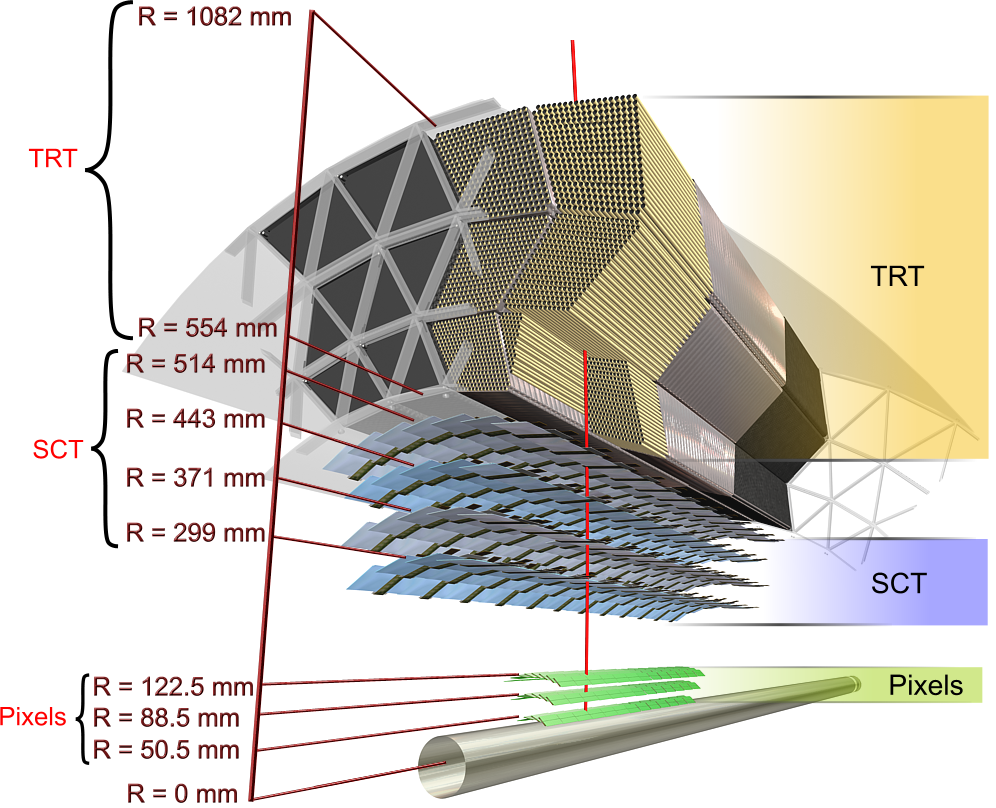
\includegraphics[width=0.6\textwidth, height=0.4\textheight]{./Images/TRD_01}
%   \end{center}
% \scriptsize
%   \itt
% \item[$\bullet$] \alert{The ATLAS transition-radiation tracker (TRT) is the
%   largest present-day TRD detector.}
% \item[$\bullet$] The TRT is part of the ATLAS inner detector and it
%   is used both for charged-particle tracking and electron/pion
%   separation. It consists of $370 000$ cylindrical drift tubes (straws).
%   Made from kapton and covered by a conductive film, the straw tube
%   serves as cathode of a cylindrical proportional drift counter.
% \item[$\bullet$] A central $30 \mu m$-diameter gold-plated tungsten
%   wire serves as anode. The layers of straws are interleaved with
%   polypropylene foils or fibres working as radiator. The tubes are
%   filled with a gas mixture.
%   \tti
% \end{frame}  

% \begin{frame}{\textcolor{Goldenrod}{Transition-Radiation Detectors}}
%   \(
%   \<{0.4\textwidth}
%   \img{TRD_02}
%   \>
%   \<{0.7\textwidth}
%   \small
%   A simiulated $ B^0_d \to J/\psi (\to e^+e^-) K_s(\pi^+\pi^-)$
%   \itt
% % \item The coordinate determination is performed by a drift-time measure-
% %   ment resulting in a spatial resolution of about $130 \mu m$.
% \item The
%   electron/pion separation is based on the energy deposition.
% \item A typical
%   energy of the transition-radiation photon in the TRT is $8 -10keV$, while
%   a minimum-ionising particle deposits in one straw about $2keV$ on
%   average
% \item \textcolor{green}{As separation parameter the number of
%   straws along the particle track having an energy deposition exceeding
%   a certain threshold can be defined.}
%   \tti
%   \>
%   \)
% \end{frame}  

% \begin{frame}{\textcolor{Goldenrod}{Transition-Radiation Detectors}}
%   \begin{center}
%     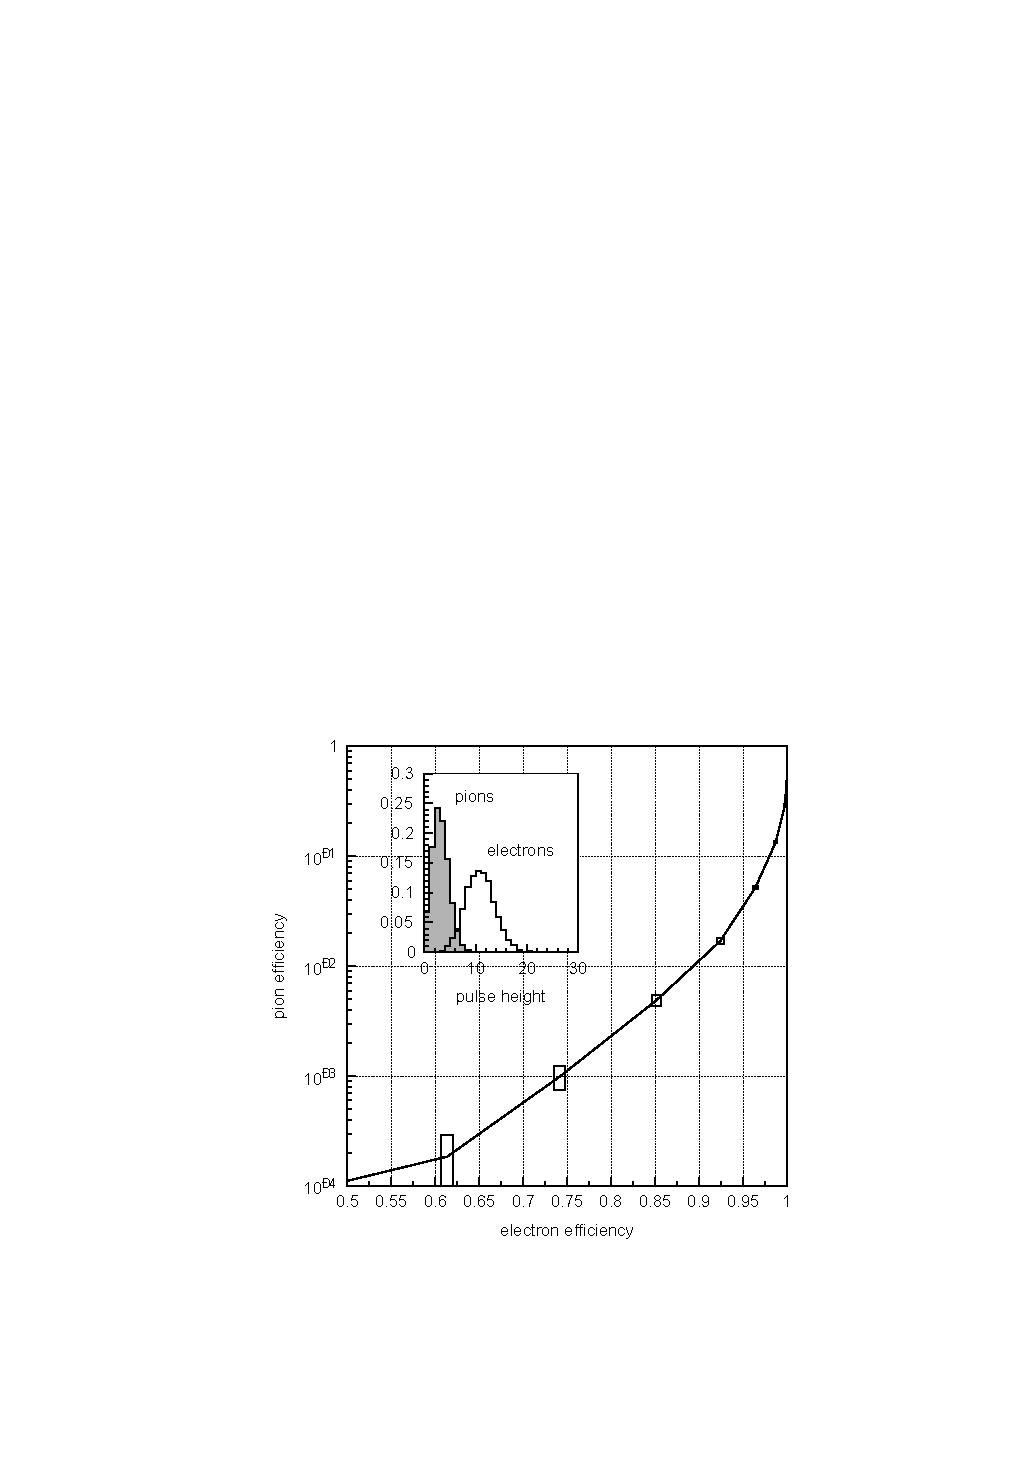
\includegraphics[width=0.6\textwidth, height=0.4\textheight]{./Images/TRD_03}
%   \end{center}
%   \textcolor{Orange}{Electron/pion separation capability measured with a prototype.
%     The insert shows the energy depositions in a single straw for pions
%     and electrons.}
% \end{frame}  



\section{Neutrino}
%%%%%%% SLIDE
\begin{frame}{\textcolor{Goldenrod}{Neutrino}}
  \note{The history of the neutrino goes back to 1914, when J. Chadwick
    first demonstrated that the beta−spectrum from the decay of a
    radioactive element was continuous, as opposed to the alpha- or
    gamma-spectrum. This seemed to imply a missing particle – or even
    possibly, as it was thought at the time, a breakdown of energy
    conservation.}
  
  \hlt{RoyalBlue}{Neutrino is so named because it is electrically neutral and
    because its rest mass is so small (-ino) that it was originally
    thought to be zero.}
  \itt
\item<2-> neutrino was postulated first by Wolfgang Pauli in
  1930 to explain how beta decay could conserve energy, momentum,
  and angular momentum (spin).
  \note{The weak force has a very short range, gravity
    is extremely weak on the subatomic scale, and neutrinos, as leptons,
    do not participate in the strong interaction}
\note{Pauli did not expect that his hypothetical new particle would ever be
  observed. However, in the early 1950s, F. Reines and C.L. Cowan Jr.,
  encouraged by B. Pontecorvo, set up a decisive experiment at the
  Savannah River nuclear reactor in South Carolina, demonstrating that
  (anti)neutrinos produced in the reactor processes sometimes interacted
  with protons in the detector medium, each reaction resulting in a
  neutron and a positron which could be registered (so-called inverse
  $\beta$-decay). This was the long awaited unambiguous proof of the existence
  of the neutrino, and in June 1956, just two years before Pauli’s
  death, Reines and Cowan could send a telegram informing Pauli of their
  discovery.}

\item<3-> neutrinos typically pass through normal matter unimpeded and
  undetected.
\item<4-> \color{red}{The assumption that neutrinos are massless and characterised by
    distinct, individual lepton numbers was incorporated into the theory
    of electro-weak interactions. }
  \tti
\end{frame}  

\subsection{Neutrino mysteries}
%%%%%%% SLIDE
\begin{frame}{\textcolor{Goldenrod}{Neutrino mysteries}}
\itt[<+->]
\item[$\Box$] \hlt{black}{Generations:} neutrinos come in three leptonic flavors
  \[
    \begin{pmatrix}
      e \\ \nu_e \\
    \end{pmatrix}
    \quad
    \begin{pmatrix}
      \mu \\ \nu_{\mu} \\
    \end{pmatrix}
    \quad 
    \begin{pmatrix}
      \tau \\ \nu_{\tau} \\
    \end{pmatrix}
  \]

\item[$\Box$] \hlt{black}{Oscillation:} \textcolor{LimeGreen}{nueutrinos
    travel through space as waves that have a different frequency. The
    flavor of a neutrino is determined as a superposition of the mass
    eigenstates. The type of the flavor oscillates, because the phase of
    the wave changes.}
\item[$\Box$] \hlt{black}{Mass:} there are three discrete neutrino
  masses with different tiny values, \alert{but they do not correspond
    uniquely to the three flavors ( $m_{\nu_{l}} < 10^{-7} m_e$)}
% \item[$\Box$] \hlt{black}{CP violation:} only left-handed neutrinos
%   participate in weak interactions.
  
  \note{In the Standard Model, lepton numbers are conserved,
    neutrinos are massless and neutrino flavours do not oscillate.}
  \tti
\end{frame}

\subsection{Neutrino sources}
%%%%%% SLIDE
\begin{frame}{\textcolor{Goldenrod}{Reactor neutrinos}}
  \begin{center}
  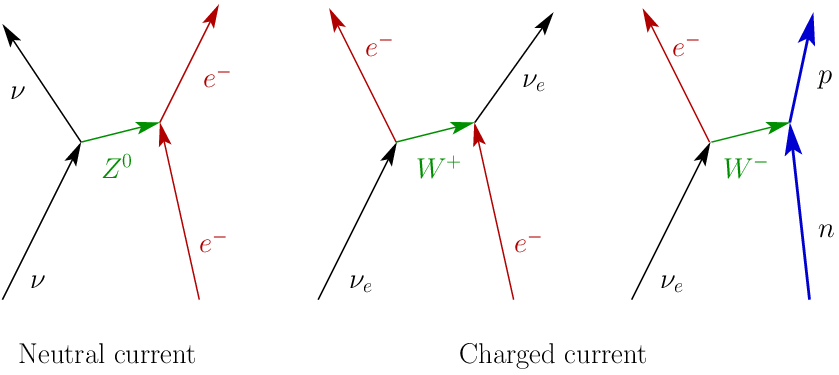
\includegraphics[width=0.6\textwidth,
  height=0.25\textheight]{./Images/neutrino_scattering}\\
  \end{center}
  \hlt{RoyalBlue}{Neutrinos participate in EW interactions}\\
  \itt
\item[$\bullet$]<2-> nuclear reactors are the major source of
  human-generated neutrinos \alert{(in $MeV$ range)} . \note{the
    majority of energy in a nuclear reactor is generated by fission
    ($^{235}U, ^{238}U, ... $)}
\item[$\bullet$]<3-> the resultant neutron-rich daughter rapidly
  undergo additional beta decays
  \[
    \begin{aligned} &n \to p \bar{\nu}_e (\beta^- decay)\\ &p \to n
      {\nu}_e (\beta^+ decay)\\ &p + e^- \to n + \nu_e (electron\, capture)
    \end{aligned}
  \]
  \note{including these subsequent decays, the average nuclear fission
    releases about $200 MeV$ of energy, of which
    roughly $4.5$\%  is radiated
    away as antineutrinos.}
  \tti
\end{frame}  

%%%%%% SLIDE 
\begin{frame}{\textcolor{Goldenrod}{Solar neutrinos}}
  %% Proton_proton_cycle
  \(
  \<{0.65\linewidth}
  \onslide<1->
  \hlt{black}{Thermonuclear fusion reactions in the solar core
    produce energy and neutrinos}
  \[
    \begin{aligned}
      & \textcolor{Blue}{p + p \to d + e^+ + \nu_e (E_{\nu} < 0.42 MeV)}\\ 
      & \textcolor{Red}{^7Be + e^- {\to} ^7Li + \nu_e (E_{\nu} < 0.86 MeV)}\\
      & \textcolor{LimeGreen}{^8B {\to} ^8Be + e^+ \nu_e (E_{\nu} < 15 MeV)}\\
      & \textcolor{Magenta}{^3He + p {\to} ^4He + e^+ + \nu_e (E_{\nu} < 18.8 MeV)} 
    \end{aligned}
  \]
  \itt
\item<3-> $pp$ chain is the dominant source in low energies and neutrinos are produced
  in $100 keV-20 MeV$ range.
  \tti
  \>
  \<{0.45\linewidth}
  \onslide<2->
  \img{Solar_neutrino_flux_spectrum}
  \>
  \)
\end{frame}

%%%%%% SLIDE 
\begin{frame}{\textcolor{Goldenrod}{Atmospheric neutrinos}}
  \(
  \<{0.3\linewidth}
  \onslide<1-> \img{atmospheric_neutrinos}
  \>
  \<{0.7\linewidth}
  \hlt{Magenta}{Neutrinos are also produced
    through cosmic nuclei-atmospheric neucli scattering (producing $\pi/
    K$)}
  \[
    \pi^{\pm}(K^{\pm}) \to \mu^{\pm} + \nu_{\mu}/\bar{\nu}_{\mu}
  \]
  \itt
\item<2-> \alert{Atmospheric neutrinos can be very energetic ($GeV$)}
  \tti
  \>
  \)
\end{frame}  

%%%%%%% SLIDE 
\begin{frame}{\textcolor{Goldenrod}{Other neutrino sources}}
  \itt
\item[$\bullet$] \hlt{blue}{Galactic and extra‐galactic:} neutrinos
  can originate from the deleptonisation phase where protons and
  electrons are merged (Supernova)
\item[$\bullet$] \hlt{blue}{Accelerator-based neutrinos:} neutrinos can be
  obtained from earthbound or cosmic accelerators in beam-dump
  experiments, where they are created in weak decays of short-lived
  hadrons.
\item \hlt{blue}{Big Bang:} the universe's neutrinos background.
  \alert{they are notoriously difficult to detect, and the $CNB$
    might never be observed directly. There is, however, compelling
    indirect evidence for its existence.}
  \tti
\end{frame}

%%%%%%% SLIDE 
\begin{frame}{\textcolor{Goldenrod}{Neutrino-nucleon scattering}}
  The cross section for neutrino-nucleon scattering of $10 GeV$
  neutrinos is on the order of $7 \times 10^{-38} cm^2/nucleon$.
  \itt[<+->]
\item Thus, for a target of $10 m$ of solid iron the interaction
  probability
  \[
    R = \sigma [N_A mol^{-1}/g \times] d\rho \approx 3\times 10^{-10}
  \]
\item \textcolor{RoyalPurple}{Neutrino–nucleon scattering of solar neutrinos of ($100 keV$) in
  the same material is $\approx 4\times 10^{-12}$}
\item Energies in the several $100keV$ range are below the
  threshold($1.8 MeV$) for inverse $\beta$ decay $(\bar{\nu}_{e} + p \to n + e^)$
  \note{ where a minimum antineutrino energy of 1.8 MeV is required to induce
    this reaction.}
\item \hlt{Red}{To get measurable interaction rates therefore high
    neutrino flux, a huge target and not too low energies are necessary.}
  \tti
\end{frame} 


%%%%%% SLIDE
\begin{frame}{\textcolor{Goldenrod}{The world's first neutrino}}
  \begin{figure}[h]
    \centering
    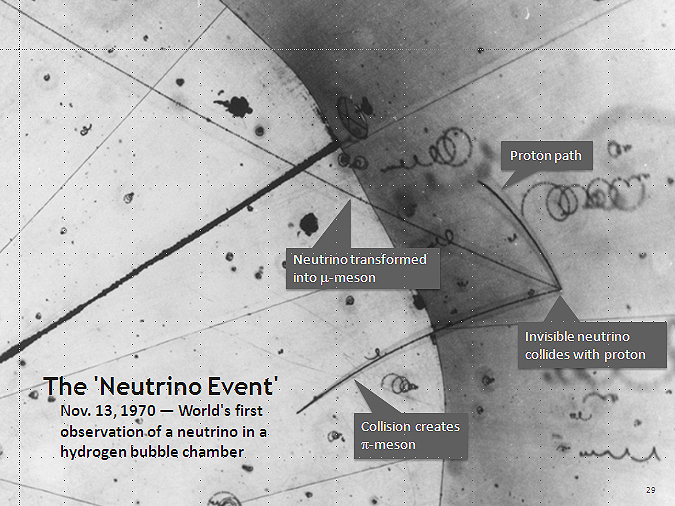
\includegraphics[width=0.85\linewidth, height=0.65\textheight]{./Images/FirstNeutrinoEventAnnotated}
    \caption*{\alert{World's first neutrino detected in a hydrogen bubble chamber (at Argonne National Laboratory)}}
  \end{figure}
\end{frame}

\section{Neutrino detectors}
%%%%% SLIDE
\begin{frame}{\textcolor{Goldenrod}{Neutrino detection techniques}}
  \note{Neutrinos are often called “ghost particles,” and for good reason.
    Neutral in charge and tiny in mass, neutrinos are incredibly elusive
    and mostly pass unnoticed through ordinary matter, including you and
    me.}
  \itt[<only@+>]
\item[$\Box$] \hlt{Orange}{Scintillators:}\\
  place a scintillation detector next to a target (solution of cadmium
  chloride in water) Antineutrinos with an energy above the threshold of
  $1.8 MeV$ undergo $IBD$ in the water. $\bar{\nu} + p \to e^+ n ; e^-
  e^+ \to \gamma \gamma$.\\
  \alert{The neutrons captured by cadmium
    nuclei resulting in delayed gamma rays that are
    detected a few microseconds after the photons from a positron
    annihilation event.}
  
  \note{Antineutrinos were first detected near the Savannah River nuclear
    reactor in 1956. Frederick Reines and Clyde Cowan used two targets
    containing a solution of cadmium chloride in water. Two scintillation
    detectors were placed next to the cadmium targets. Antineutrinos with
    an energy above the threshold of 1.8 MeV caused charged current
    "inverse beta-decay" interactions with the protons in the water,
    producing positrons and neutrons. The resulting positron annihilations
    with electrons created pairs of coincident photons with an energy of
    about 0.5 MeV each, which could be detected by the two scintillation
    detectors above and below the target. The neutrons were captured by
    cadmium nuclei resulting in delayed gamma rays of about 8 MeV that
    were detected a few microseconds after the photons from a positron
    annihilation event.}

  \item[$\Box$] \hlt{Orange}{Radiochemical methods:}\\
    based on the method suggested by Bruno Pontecorvo, consist of a
    tank filled with a chlorine containing fluid such as
    tetrachloroethylene.\\
    \hlt{Red}{A neutrino converts a chlorine-37 atom
      into one of argon-37 via the charged current interaction.}
    
  \item[$\Box$]  \hlt{Orange}{Cherenkov(RICH) detectors:}\\
    detect Cherenkov light of muon or electron.\\
    \textcolor{Magenta}{In a Cherenkov detector, a large volume of clear
      material such as water or ice is surrounded by light-sensitive
      photomultiplier tubes.}
    
  \item[$\Box$]  \hlt{Orange}{Tracking calorimeters:}\\
    use alternating planes of absorber material and detector material.
    The absorber planes provide the energy while the detector planes
    provide the tracking information.\\
    Steel is a popular absorber choice,
    being relatively dense and inexpensive and having the advantage that
    it can be magnetised. \\
    \hlt{Red}{Tracking calorimeters are only useful
      for high-energy (GeV range) neutrinos.}\\
    \hlt{ForestGreen}{At these energies, neutral current interactions appear as a shower
      of hadronic debris and charged current interactions are identified
      by the presence of the charged lepton's track (possibly alongside
      some form of hadronic debris.)}
    
    \note{The NOVA proposal suggests eliminating the absorber planes
    in favor of using a very large active detector volume. The active
    detector is often liquid or plastic scintillator, read out with
    photomultiplier tubes, although various kinds of ionisation chambers
    have also been used.}
\tti
\end{frame}

\subsection{Homestake experiment}
%%%%%%% SLIDE 
\begin{frame}{\textcolor{Goldenrod}{Homestake experiment}}  
  % Ray_Davis_exp
  \note{The Homestake Mine was a deep underground gold mine located in Lead,
    South Dakota.}
  \itt[<+->]
\item[$\bullet$] The Homestake experiment ($1965-1967$, radiochemical)
  led by Raymond Davis, Jr. 
  looked for solar neutrinos above $0.814 MeV$ through IBD
  \[
    \nu_e + ^{37}Cl \to ^{37}Ar + e^- 
  \]

\item \hlt{Red}{The Homestake detector observed less than $1/3 SNU$
    (One solar neutrino unit $=$ one interaction per $10^{36}$ target atoms
    $s^{-1}$.) than it expected}
  
% \item[$\bullet$] \hlt{Magenta}{the cross section is greatly
%     enhanced above $5.8 MeV \to $ chlorine experiment sensitive to the
%     energetic$^8{B}$-neutrinos}
%   \note{due to the transition of the ground state of
%     the $^{37}Cl$ nucleus to its isobaric analog state in $^{37}Ar$,
%     making the chlorine experiment particularly sensitive to the energetic
%     neutrinos from $^8B$ decay (Bahcall 1964).}
% \item[$\bullet$] \hlt{Green}{large-scale $^{37}Cl - ^{37}Ar$ radiochemical detector
%     can observe a measurable flux of neutrinos.}
  \tti  
\end{frame}


\subsection{GALLEX experiment}
%%%%%%% SLIDE
\begin{frame}{\textcolor{Goldenrod}{GALLEX experiment}}
  %% cite The GALLEX solar neutrino experiment
  \hlt{black}{The radiochemical GALLium EXperiments (GALLEX) looked
    for the solar $pp$ neutrinos $(1991-1995)$.}
  \itt
\item GALLEX monitored solar neutrinos above $233 KeV$ through
  \[
    ^{71}Ga + v_e \to e^- + ^{71}Ge
  \]
\item<2-> \hlt{Magenta}{$^{71}Ge$ ($\tau_{1/2} = 11.43 days$) (through electron-capture)
  emits Auger electrons and X-rays }
\item<3-> scatter solar neutrinos from the $^{71}Ga$ target while holding
  the BKG as low as possible.
\item<3-> extract $^{71}Ge$ and transform them into a proportional chamber
  and count them.  
\tti
\end{frame}  

%%%%%% SLIDE
\begin{frame}{\textcolor{Goldenrod}{GALLEX: detector}}
  \(
  \<{0.4\textwidth}
  \img{GALLEX01}
  \>
  \<{0.7\textwidth}
  \itt
%\item[$\bullet$] located 120 km east of Rome, $h= 8m ;  r = 1.9 m$.
\item[$\bullet$] $30.3$ tons of $GaCl_3$ ($8.2 M/l GaCl_3$ and $1.9
  M/l$ of $HCl$) in a cylinder($h= 8m ;r = 1.9 m$)
\item[$\bullet$] gemrmanium is extracted by a large flow ($300 m^3/h$) of $N_2$
  \note{in the form of $GeCl_4$ (very volatile in the presence of $HCl$),
  therefore it's flushed out with $N_2$ and then absorbed into pure
  water. It's then transformed into $GeH_4$ and put into a small
  proportional counter.}
  
\item[$\bullet$]<2-> A typical solar exposure lasts about one month (followed by a
  6-month period of counting $^{71}Ge$)
\item[$\bullet$]<3-> \hlt{Red}{$^{51}Cr$ has been chosen as a convenient source of $\nu$
  (through e-capture of $^{50}Cr$) with the flux of $\approx 6\times
  10^{16} \nu/s$ in order validate the whole experiment.}
\tti
\>
\)
\end{frame}

%%%%%%% SLIDE
% \begin{frame}{\textcolor{Goldenrod}{The GALLEX}}
%   \begin{figure}[h]
%     \centering
%     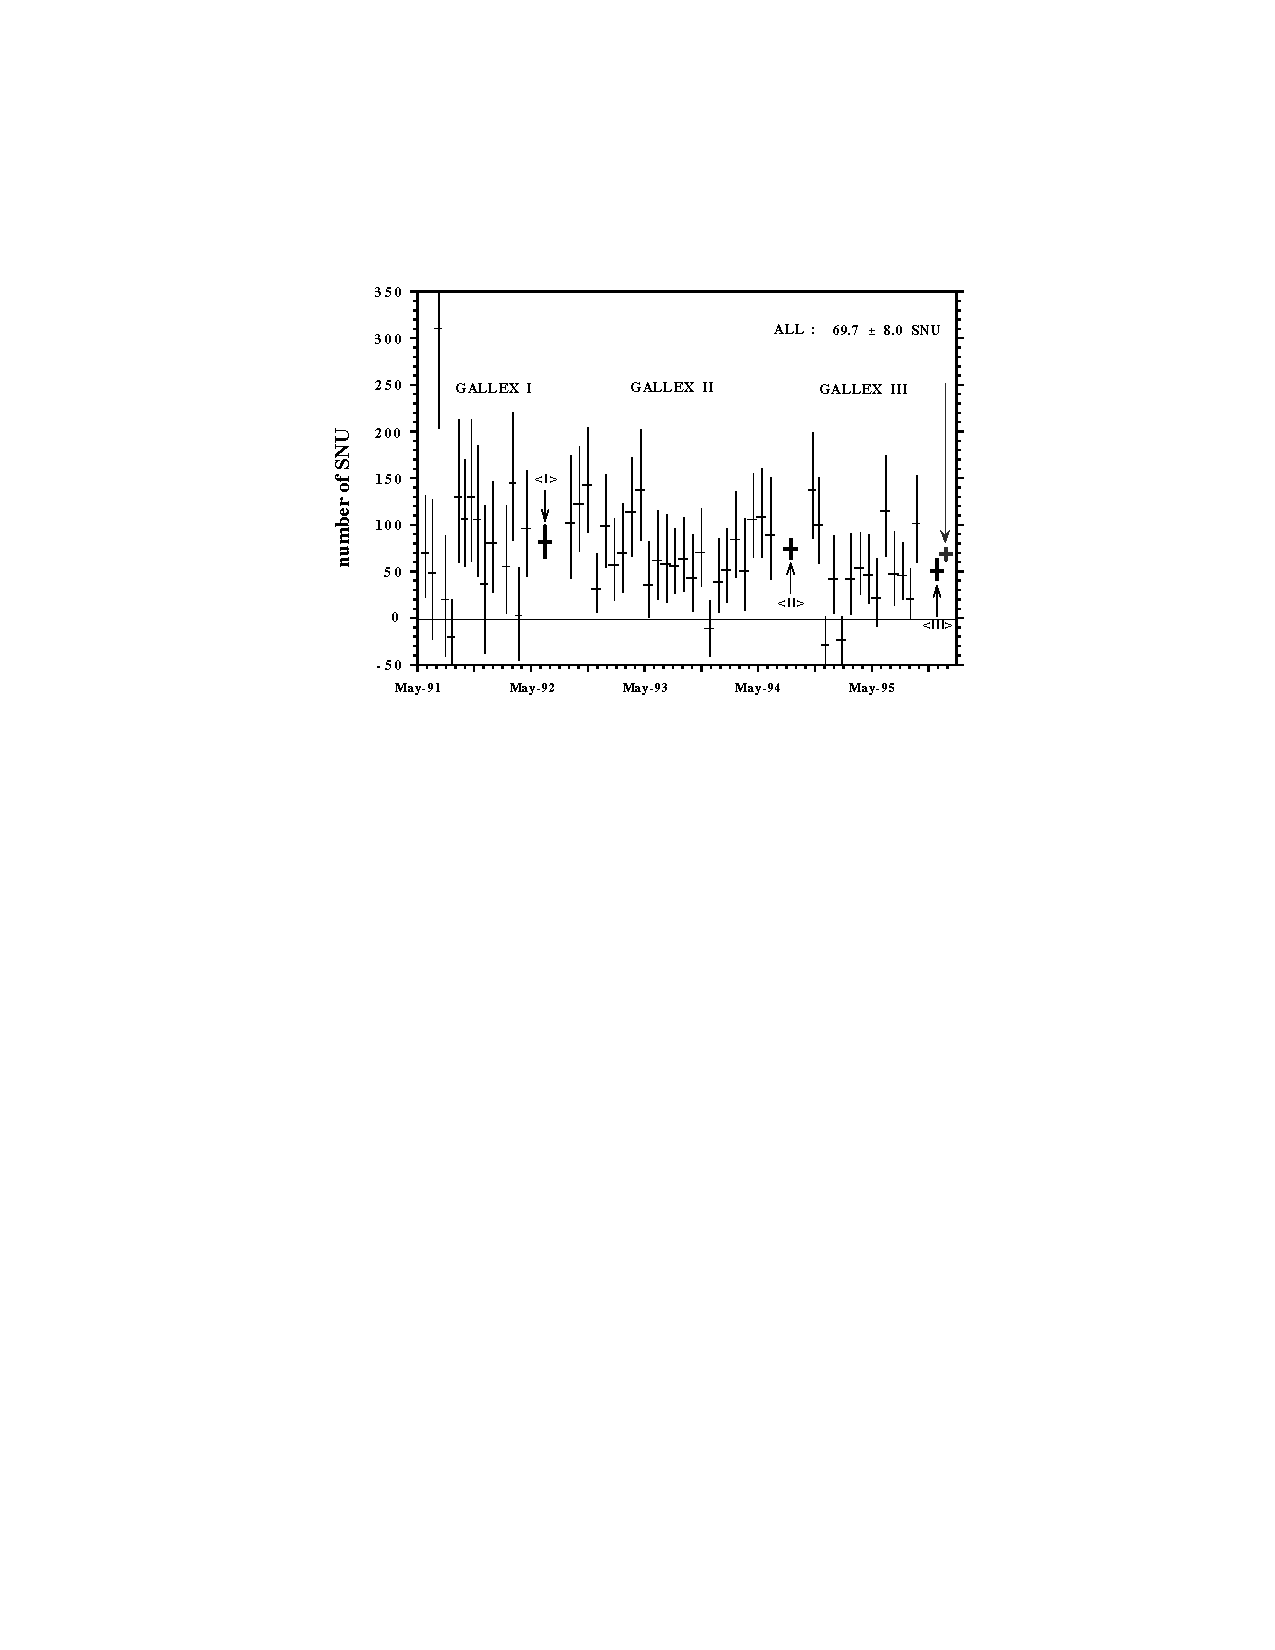
\includegraphics[width=0.7\linewidth, height=0.5\textwidth]{./Images/GALLEX02}
%     \caption*{Results of the 53 GALLEX solar runs together with the
%       combined value}
%   \end{figure}
% \end{frame}

%%%%%% SLIDE 
\begin{frame}{\textcolor{Goldenrod}{The GALLEX}}
  \begin{figure}[h]
    \centering
    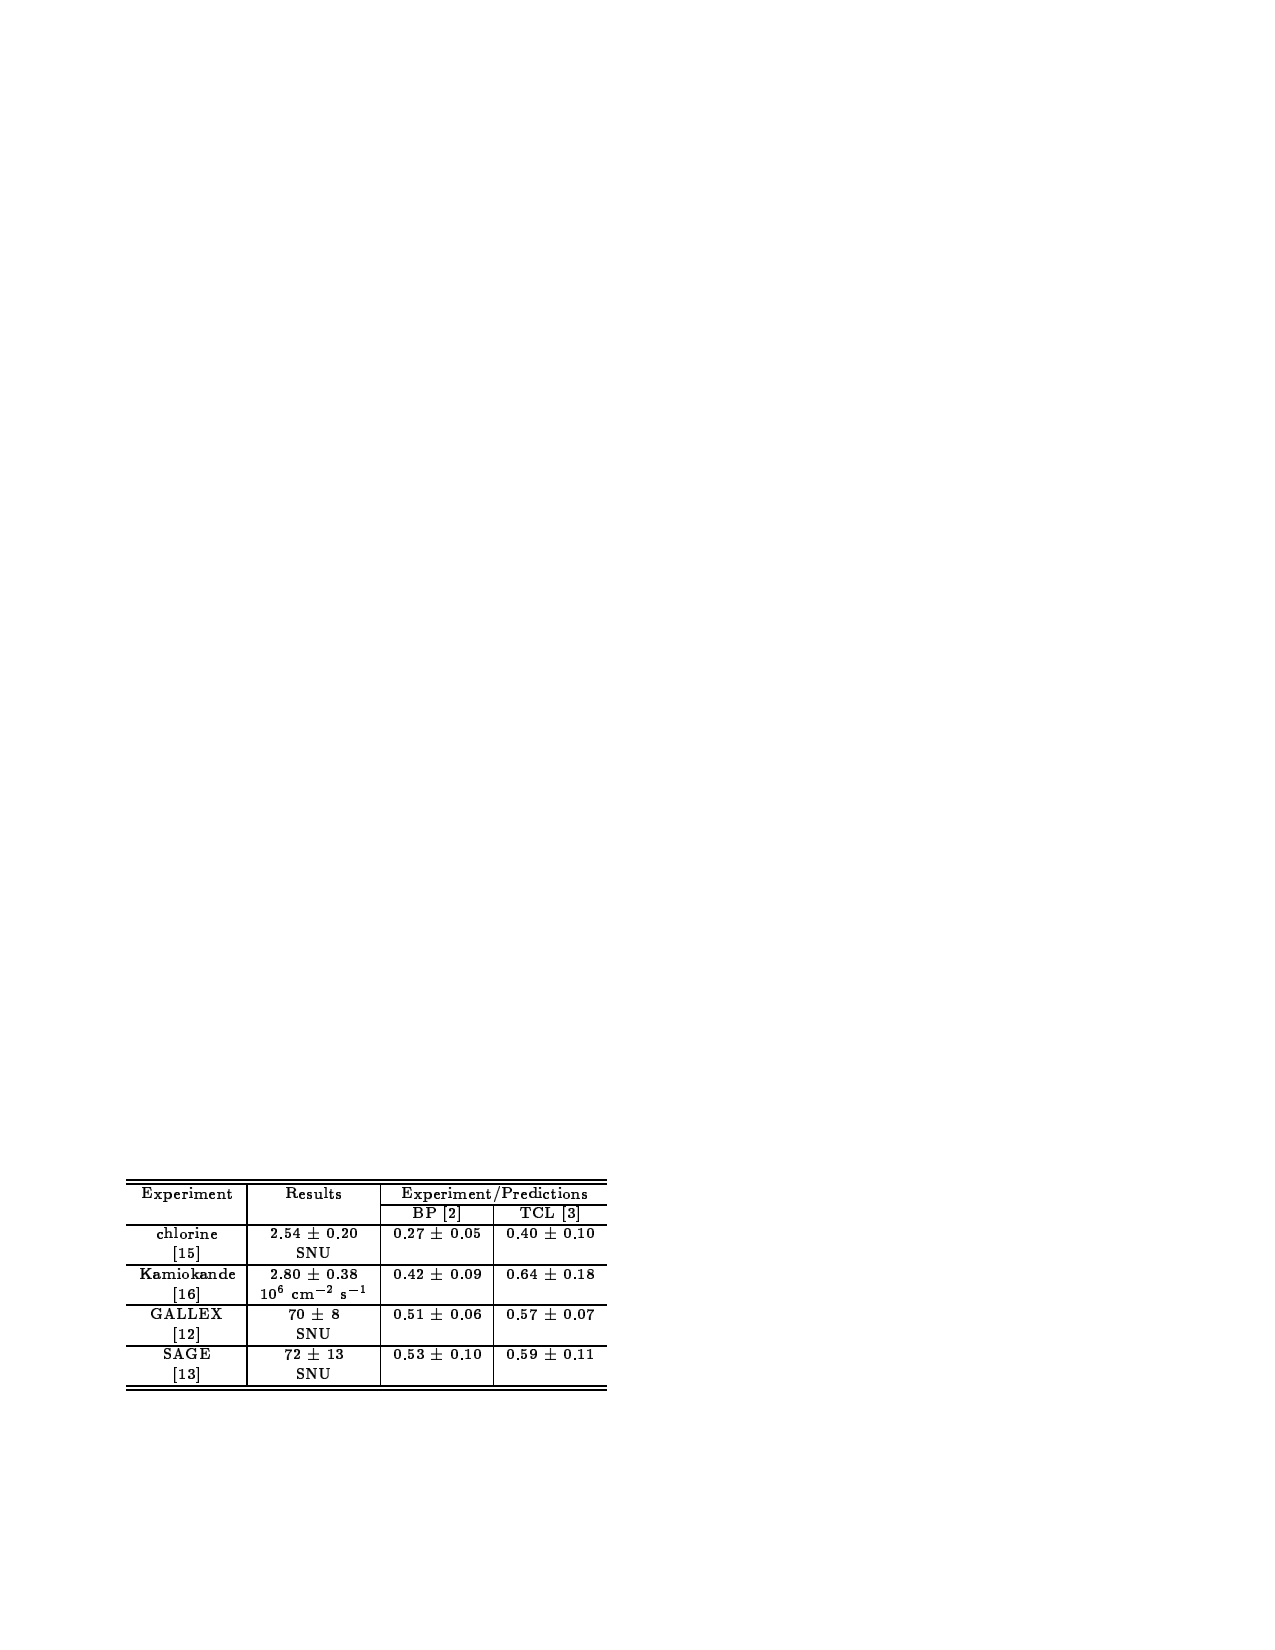
\includegraphics[width=0.6\linewidth, height=0.3\textheight]{./Images/GALLEX03}
    \caption*{Results of the solar neutrino experiments and comparison
      to the predictions from Bahcall and Pinson (BP) and Turck-Chieze
      and Loops (TCL).
    }
  \end{figure}
  \itt
\item<2-> Chlorine is mainly sensitive to the $\nu_{Be} and \nu_B$,
  Kamiokande to $\nu_B$ and GALLEX is sensitive to $\nu_{pp}$
\item<3-> \hlt{Red}{deficit in all experiments shows something
    fundamental is missing} $\to$
  {\it \textcolor{Magenta}{neutrino oscillation turned out to be the reason.}}
  \tti
\end{frame}

\subsection{Calorimetric neutrino detectors}
%%%%%%% SLIDE
\begin{frame}{\textcolor{Goldenrod}{Calorimetric neutrino detectors}}
  \hlt{RoyalPurple}{Calorimetric neutrino detectors for high-energy neutrinos are based
    on the measurement of the total energy of the final-state hadrons
    produced in a neutrino–nucleon interaction.}
  
  \itt
\item<2-> These calorimeters are
  mostly sandwiches consisting of alternating passive targets and
  active detectors

  \note{ (e.g. scintillators) like those being used for
  hadron calorimeters. Of course, also total-absorption calorimeters
  can be built, where the target at the same time must be an active
  detector element.}

\item<3-> The large neutrino detectors at CERN (CDHS and
  Charm) were sampling detectors while KARMEN and SuperKamiokande are
  large-volume total-absorption devices
  
  \note{exploiting Cherenkov and
    scintillation-light detection.}
  
\item<4-> \alert{Depending on which neutrino flavour
  is being detected the calorimeter must be sensitive not only to
  hadrons but also to electrons or muons.}
\tti  
  % CERN  
  % DORTMUND  
  % HEIDELBERG  
  % SACLAY  
  % WARSAW
  
\end{frame}


\subsection{NOMAD experiment}
%%%%%%% SLIDE
\begin{frame}{\textcolor{Goldenrod}{NOMAD experiment}}
  \hlt{Orange}{A precise knowledge of the cross section of (anti)neutrino-nucleus
    quasi-elastic scattering process (QEL) is important for the planning
    and analysis of any experiment which detects astrophysical,
    atmospheric or accelerator neutrinos.}
  
  \note{The available measurements
    from early experiments at ANL , BNL , FNAL , CERN
    and IHEP  have considerable errors due to low
    statistics and a lack of knowledge of the precise incoming neutrino
    flux. Unfortunately, even within these large errors, the results are
    often conflicting.}
  
  \itt
\item[$\Box$]<2-> Neutrino Oscillation MAgnetic Detector (NOMAD)
  investigated the QEL process
  \[
    \begin{aligned}
      &\nu_{\mu} + n \to \mu^- + p \\
      &\bar{\nu}_{mu} + p \to \mu^+ + n
    \end{aligned}
  \]
\item[$\Box$]<3-> The main goals of the NOMAD experiment:
  \itt
\item<3-> probing necluon internal structure and neutrino
  oscillations
  \tti
  \tti
\end{frame}


%%%%%%%%  SLIDE
\begin{frame}{\textcolor{Goldenrod}{NOMAD experiment: neutrino beam}}
  \begin{overlayarea}{\textwidth}{\textheight}
  \begin{figure}[h]
    \centering
    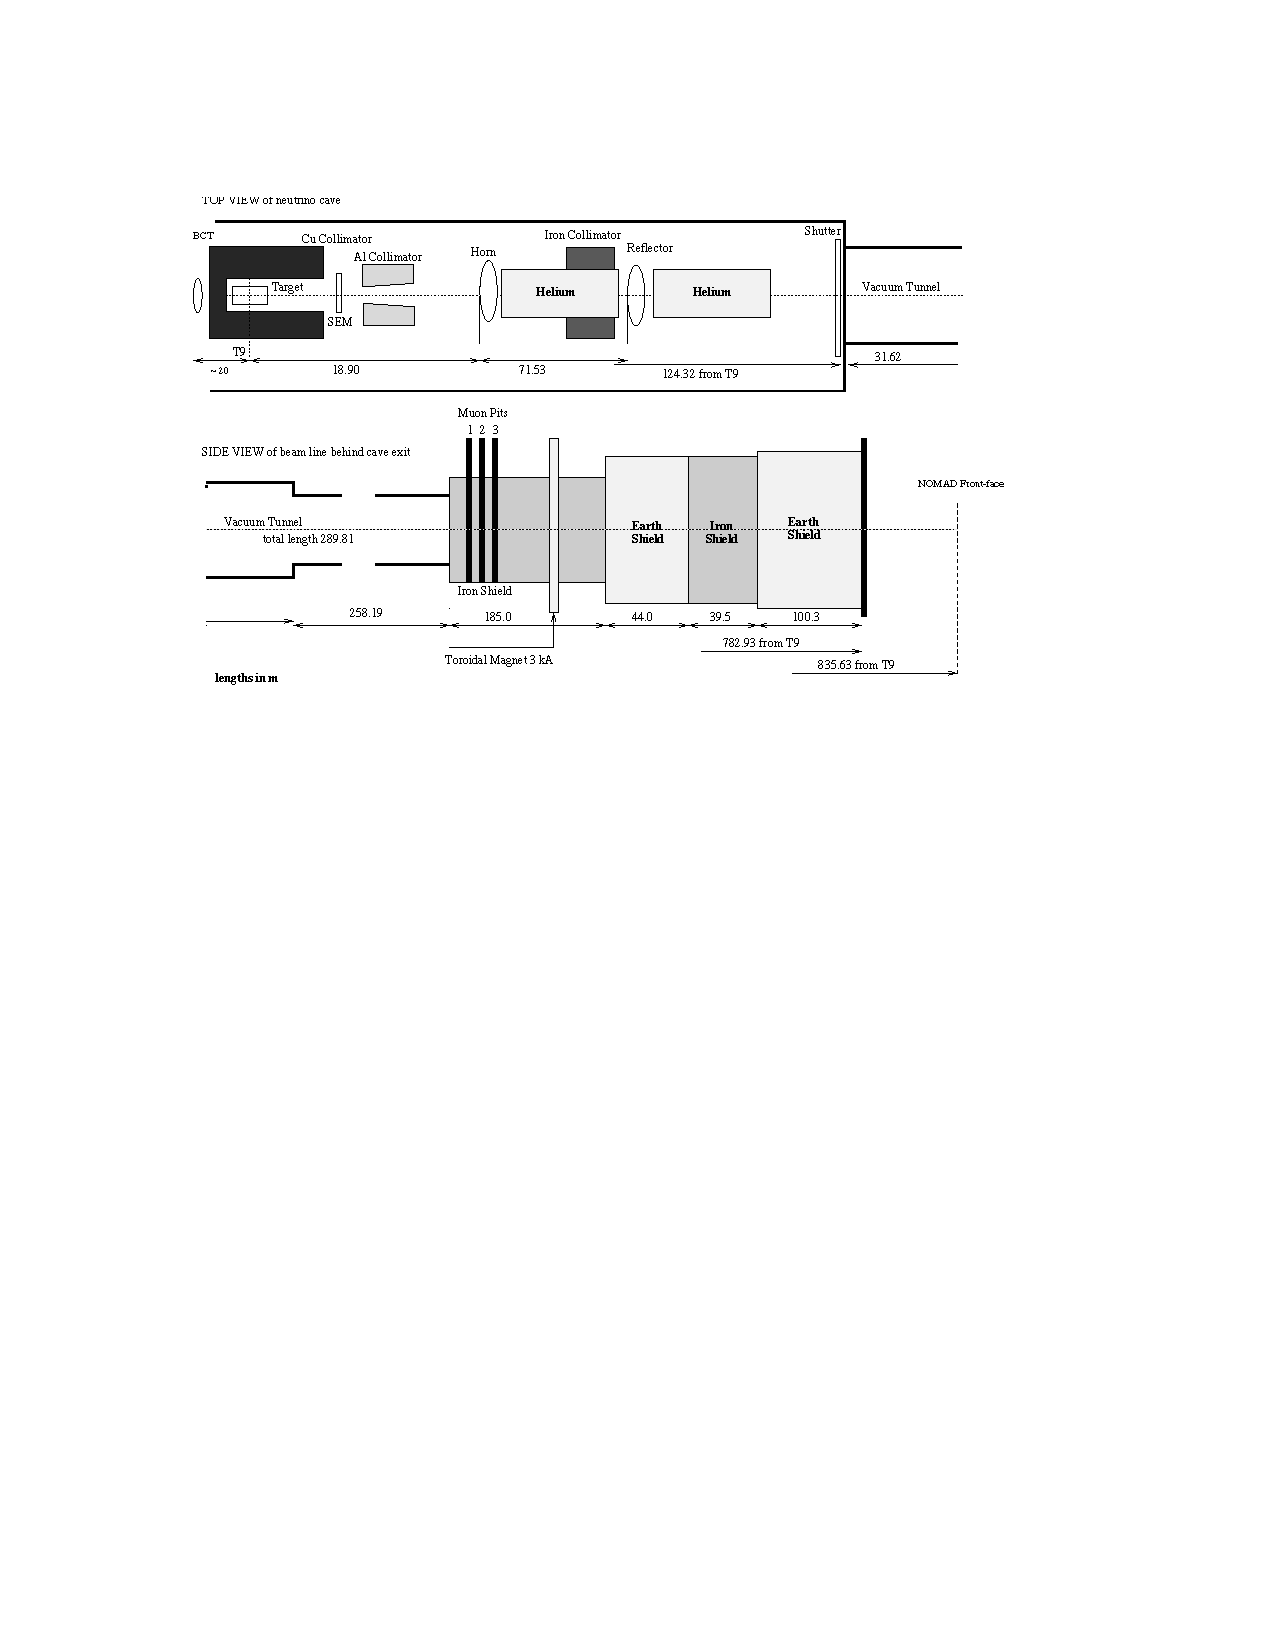
\includegraphics[height=0.35\textheight, width=0.7\linewidth]{./Images/NOMAD03}
    \caption*{The general layout of the beam line}
  \end{figure}
  \itt[<only@+>]
\item $450 GeV$ proton beam hits a beryllium target $\to$
  \textcolor{Magenta}{charged particles (mainly $\pi^+$ and $K^+$
    mesons) produced around zero degrees subsequently decay producing
    neutrinos.}
  
% \item A large
%   iron and earth shield placed at the end of the decay volume filters
%   out particles other than neutrinos and is followed by the detector,
  
\item mainly of $\nu_{\mu}$ (
  with an about $7$\% admixture of $\bar{\nu}_{\mu}$ and less than
  $1$\% of $\nu_e/bar{\nu}_e$.
  \tti
 \end{overlayarea} 
\end{frame}


%%%%%% SLIDE 
\begin{frame}{\textcolor{Goldenrod}{NOMAD experiment: detector}}
  \begin{overlayarea}{\textwidth}{\textheight}
    \begin{figure}[h]
    \centering
    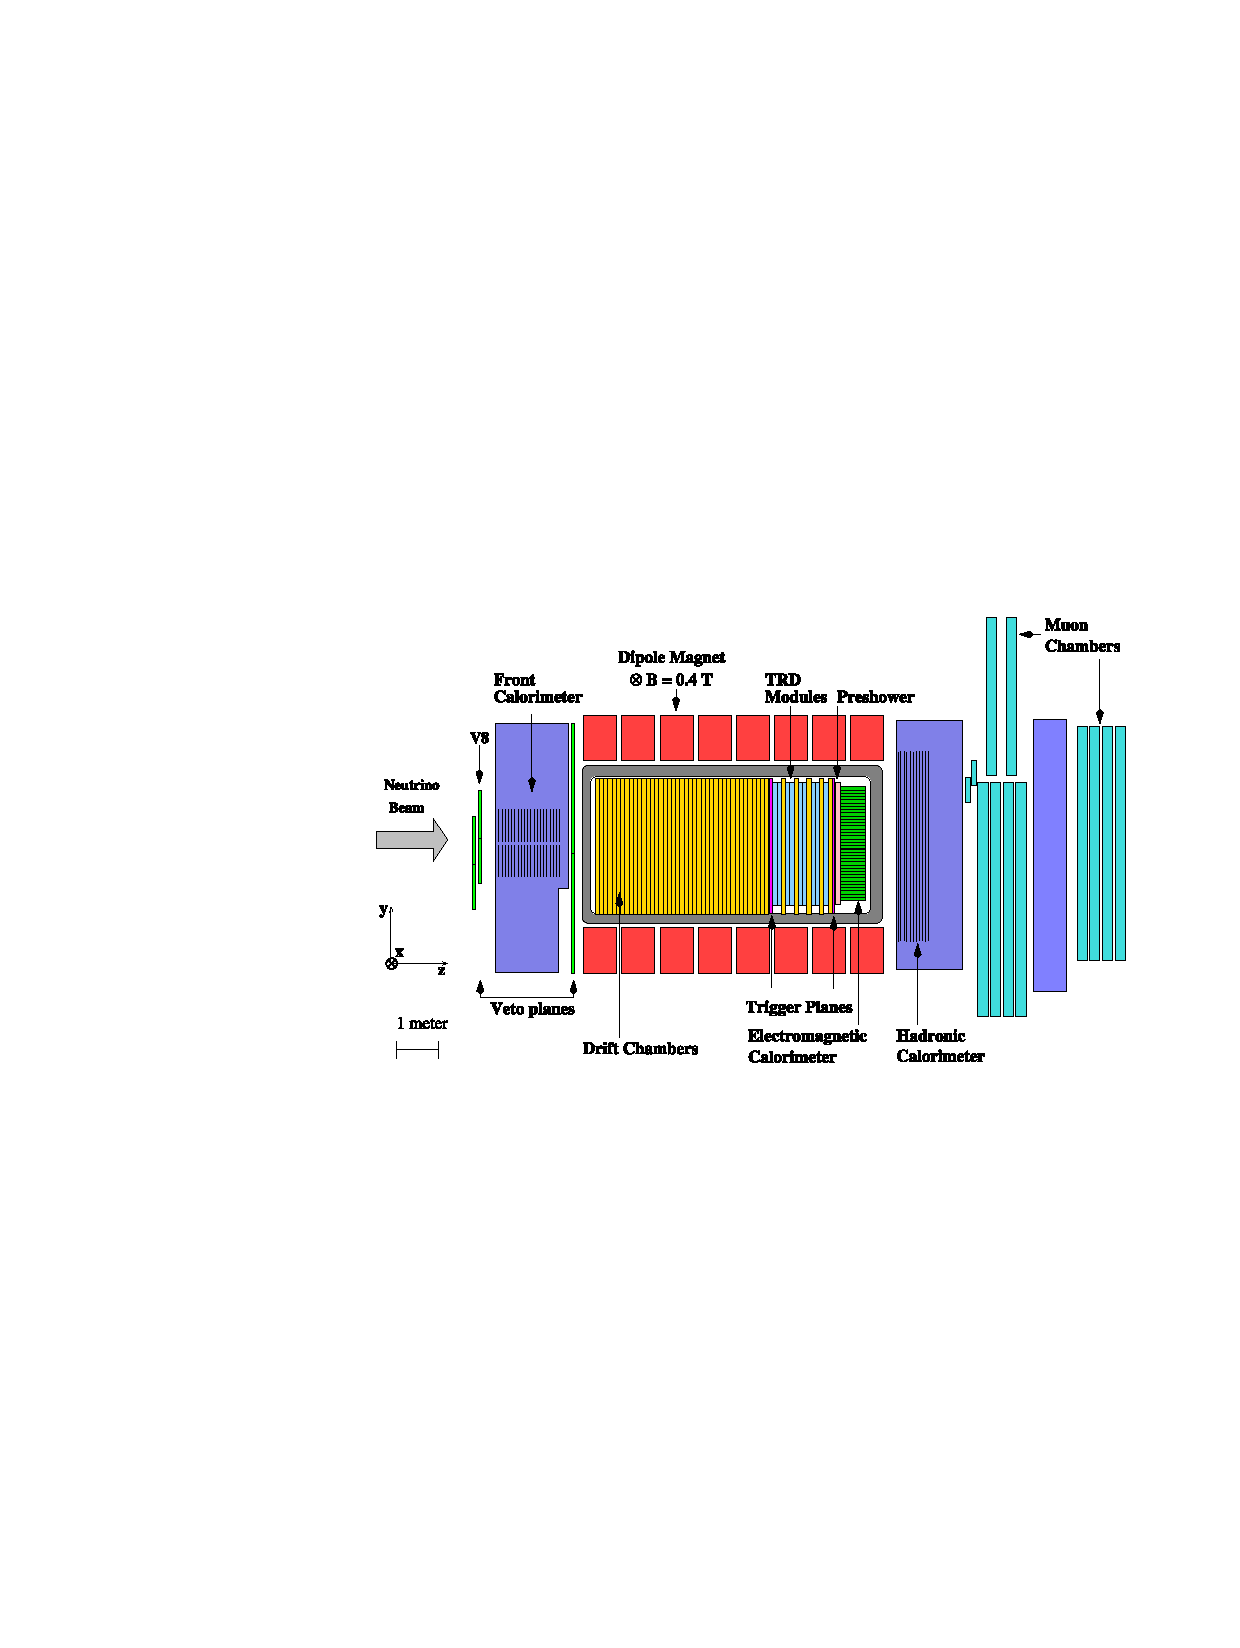
\includegraphics[height=0.4\textheight, width=0.8\linewidth]{./Images/NOMAD01}
  \end{figure}
  \itt[<only@+>]
\item The NOMAD detector consisted of an active target of $44$ drift
  chambers with a total fiducial mass of $2.7 tons$, located in a $0.4$
  Tesla dipole magnetic field. The total volume of the drift chambers is
  about $ 3 \times 3\times 4 m^3$)
\item Drift chambers, made of low $Z$ material served the dual
    role of a nearly isoscalar target1 for neutrino interac- tions and of
    tracking medium.

  \note{The average density of the drift chamber volume was 0.1 g/cm3.
    These chambers pro- vided an overall efficiency for charged track
    reconstruction of better than 95\% and a momentum resolution which can
    be approximated by the following formula $\frac{\sigma_p}{p} \approx
    \frac{0.05}{\sqrt{L}}$}
  
\item Reconstructed tracks were used to determine the event topology
  (the assignment of tracks to vertices), to reconstruct the vertex
  position and the track parameters at each vertex and, finally, to
  identify the vertex type (primary, secondary, etc.).
  
\item A transition radiation detector (TRD) placed at the end of the
  active target was used for particle identification. Two scintillation
  counter trigger planes were used to trigger on neutrino interactions
  in the NOMAD active target.
\item A lead-glass electromagnetic calorimeter located downstream of
  the tracking region provided an energy resolution of $3.2/\sqrt{E}
  \oplus 1$\% for electromagnetic showers and was crucial to measure the
  total energy flow in neutrino interactions.

\item In addition, an iron absorber and a set of muon chambers located
  after the electromagnetic calorimeter was used for muon
  identification, providing a muon detection efficiency of 97\% for
  momenta greater than $5 GeV/c$.
  \tti
\end{overlayarea}
\end{frame}

%%%%%% SLIDE
\begin{frame}{\textcolor{Goldenrod}{NOMAD experiment: results}}
  \begin{overlayarea}{\textwidth}{\textheight}
  \begin{figure}[h]
    \centering
    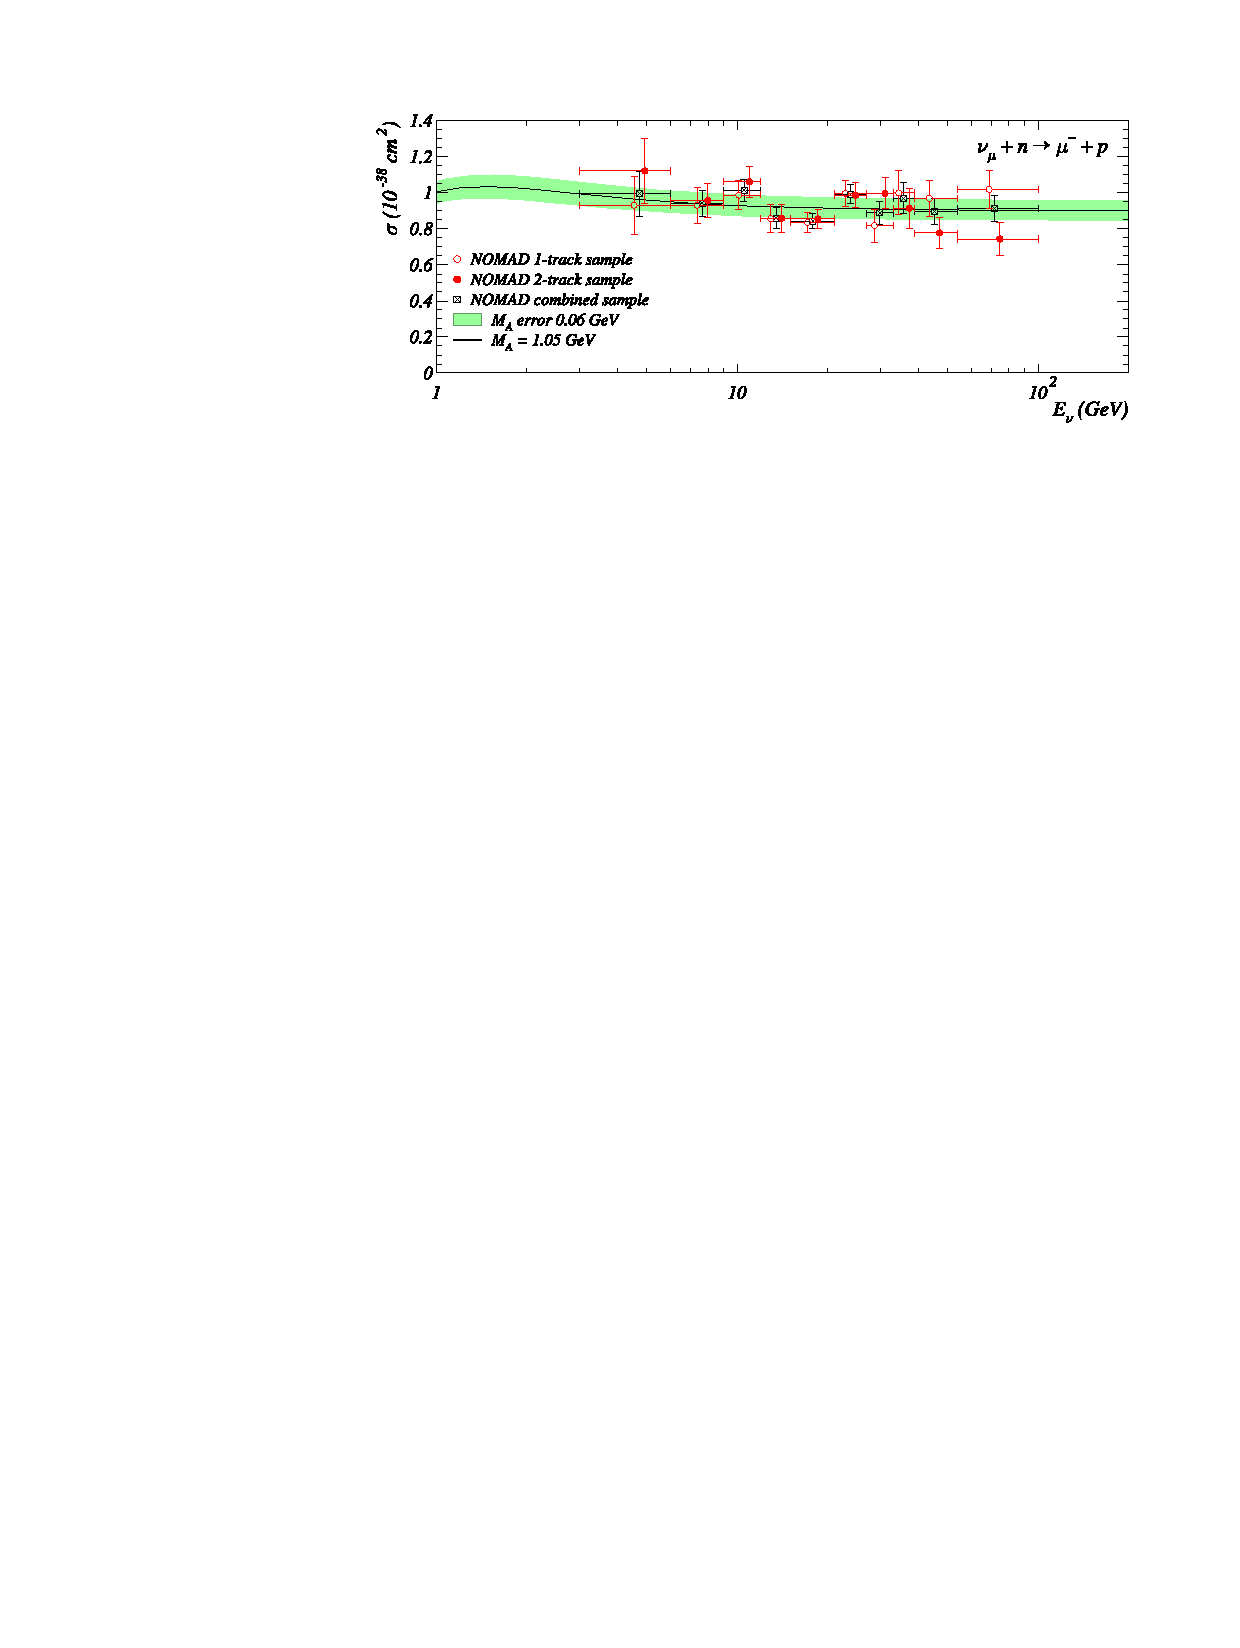
\includegraphics[height=0.4\textheight, width=0.8\linewidth]{./Images/NOMAD04}
    \caption*{$\nu_{\mu} + n \to \mu^- + p$ quasi-elastic scattering cross-section}
  \end{figure}
  
  %%\hlt{black}{Significance of $\nu-$nucleon QEL:}
  \itt[<only@+>]
\item the axial structure of the nucleon. Provide information on
  spin-isospin distributions (i.e. they can discriminate between
  'upness' and 'downness') Provide insight into the differences between
  proton and neutron structure Isospin symmetry violation Strangeness
  contributions.
% \item for the region of low and intermediate 4-momentum transfer,
%   $Q^2$, we can use a dipole parameterization for the axial form factor
%   with only one adjustable parameter, the so-called axial mass $M_A$
% \item the $M_A$ parameter describes the internal structure of the
%   nucleon and should be the same both for neutrino and antineutrino
%   experiments
% \item extract the MA parameter from experimental data with the fit
%   of the $Q^2$ distribution of the identified neutrino QEL events.
  \tti 
\end{overlayarea}
\end{frame}


\subsection{Super-Kamiokande experiment}
%%%%%% SLIDE
\begin{frame}{\textcolor{Goldenrod}{Super-Kamiokande experiment}}
    %\begin{overlayarea}{\textwidth}{\textheight}
    \begin{figure}[h]
      \centering
      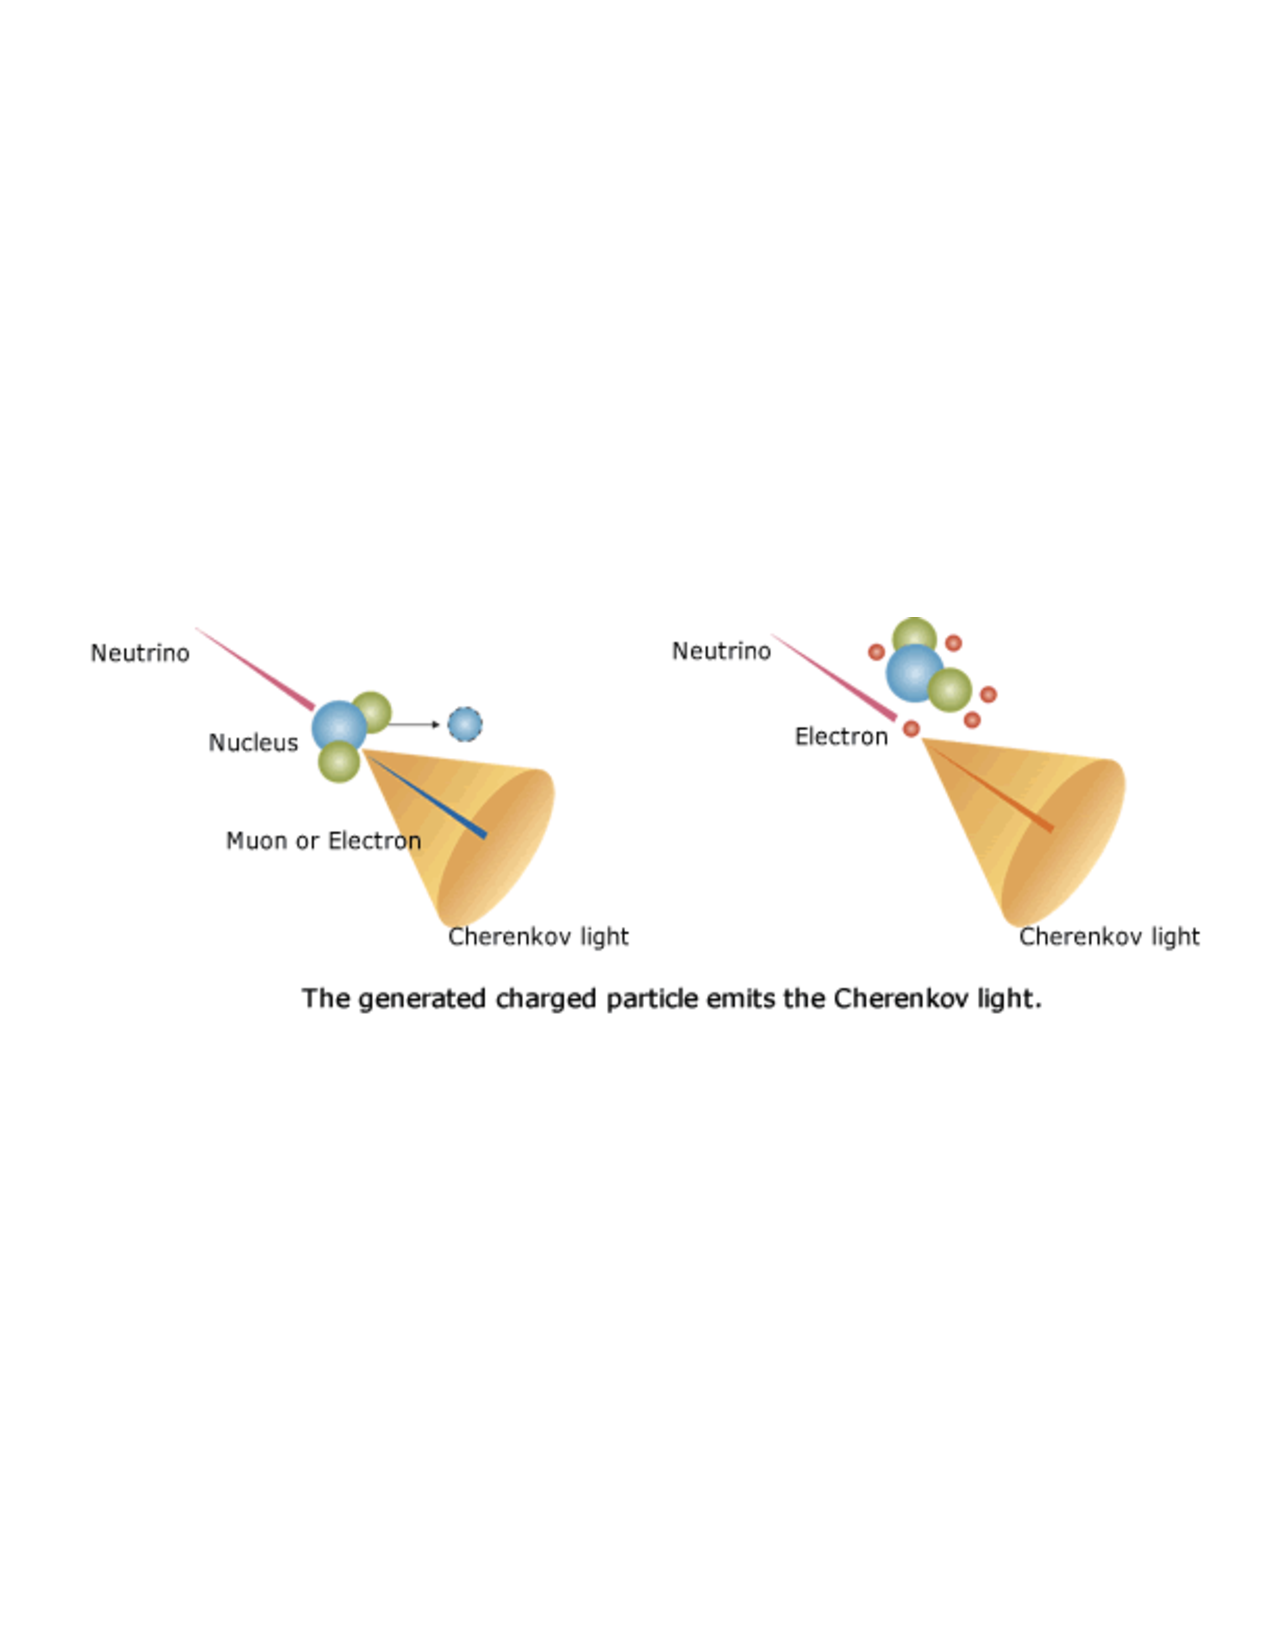
\includegraphics[height=0.2\textheight]{./Images/SKK04.pdf}
    \end{figure}
    
    \itt
  \item signals:
    \[
      \begin{split}
        &\nu_{l} + e^- \to \nu_l + e^- (ES)\\
        &\nu_l + p \to l^-  + n  (CC)\\
      \end{split}
    \]
    
  \item \hlt{black}{Physics aims}:\\
    $-$ neutrino oscillation\\
    $-$ neutrinos mass\\
    $-$ neutrino flavors 
    % \hlt{Magenta}{unsolved neutrino mysteries: the CP violation
    % parameter, the neutrino mass hierarchy and mass value of each
    % neutrino.}
    % \item searches: solar neutrinos, atmospheric neutrinos, proton decay
    %   and neutrinos from Supernova burst.
    \tti
\end{frame}

%%%%%% SLIDE
\begin{frame}{\textcolor{Goldenrod}{Super-Kamiokande experiment: detector}}
  \begin{overlayarea}{\textwidth}{\textheight}
  \begin{figure}[h]
    \centering
    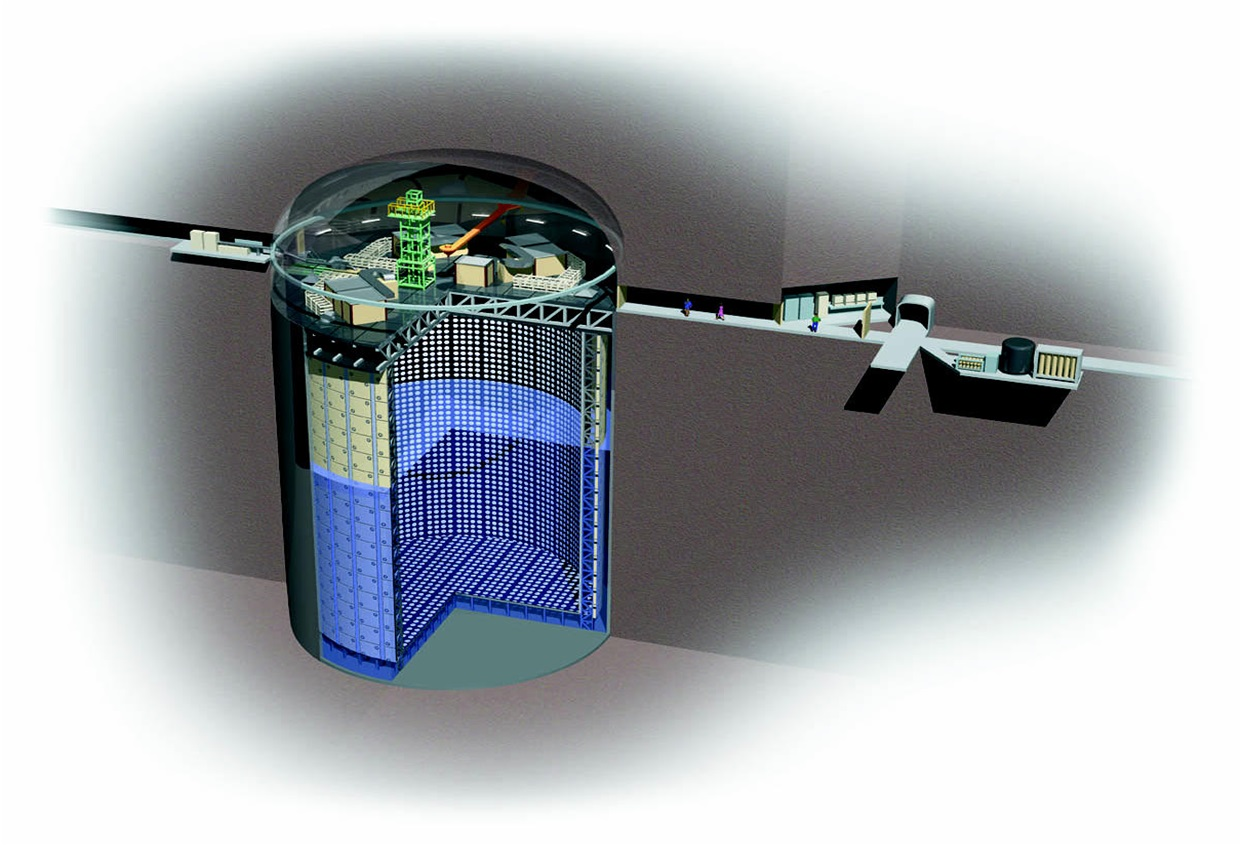
\includegraphics[height=0.4\textheight]{./Images/SKK06}
  \end{figure}
  \itt[<only@+>]
  \note{ The $50000$ tons of water as a big target can
  increase the number of interaction between neutrinos and nucleons or
  electrons. $13000$ eyes watch Cherenkov light}

\item[$\bullet$] \hlt{Orange}{Water tank:}\\
  The Super-Kamiokande detector consists of a cylindrical stainless
  steel tank, $39.3m$ in diameter and $41.4m$ in height filled with
  $50 ktons$ of pure water.
  
\item[$\bullet$] \hlt{Orange}{ID:}\\
  \small $11129$ ($20-inch$) inward-facing PMTs are evenly placed on the wall of
    the ID\\
    {\small in order to protect the detector against PMT implosions as
      happened in 2001, each ID PMT is enclosed in a FRP housing with an
      acrylic window covering the photocathode area so that the shock wave
      does not occur even if one of the PMTs imploded.}

  \note{The spaces on
    the ID wall between the PMTs are covered with opaque black sheets made
    of polyethylene terephthalate ensuring the ID and the OD are optically
    well separated.}
\item[$\bullet$] \hlt{Orange}{OD:}\\
  \small 1,885 (8-inch) evenly-spaced PMTs
    facing outward.\\
    {\small Unlike the ID, the spaces between
      the PMTs are covered with a reflective material Tyvek which has
      about 90\% reflectivity at 400 nm in order to increase the photon
      collection efficiency in the OD.}
    
  \item[$\bullet$] \textcolor{Magenta}{each PMT is surrounded by  square
      wavelength-shifting plates to transfer Cherenkov UV to visible light}
  \tti
\end{overlayarea}
\end{frame}

%%%%%% SLIDE
\begin{frame}{\textcolor{Goldenrod}{Super-Kamiokande experiment: an
      event display}}
  \begin{figure}[h]
    \centering
    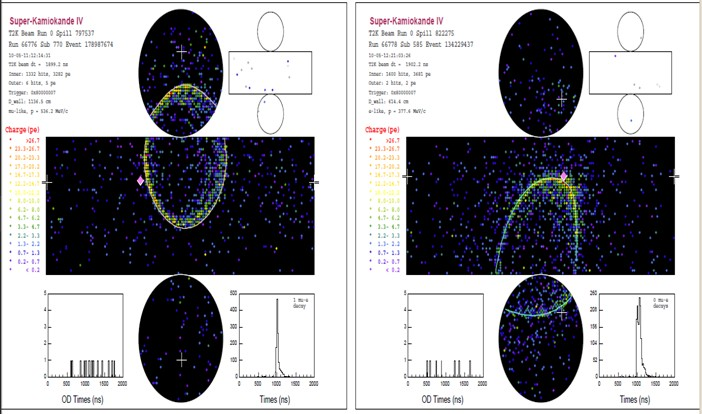
\includegraphics[height=0.4\textheight]{./Images/SKK100}
  \end{figure}
  \itt
\item \textcolor{Magenta}{electron(left) and muon(right) events in the atmospheric
    neutrino data. The ring for muon is sharper than electron}

\item Each dot represents a PMT which detected Cherenkov photons,
  and the colour scale represents the number of photons detected at each PMT.
  \tti
\end{frame}

%%%%%% SLIDE
\begin{frame}{\textcolor{Goldenrod}{Super-Kamiokande experiment: results}}
  \begin{overlayarea}{\textwidth}{\textheight}
  \begin{figure}[h]
    \centering
    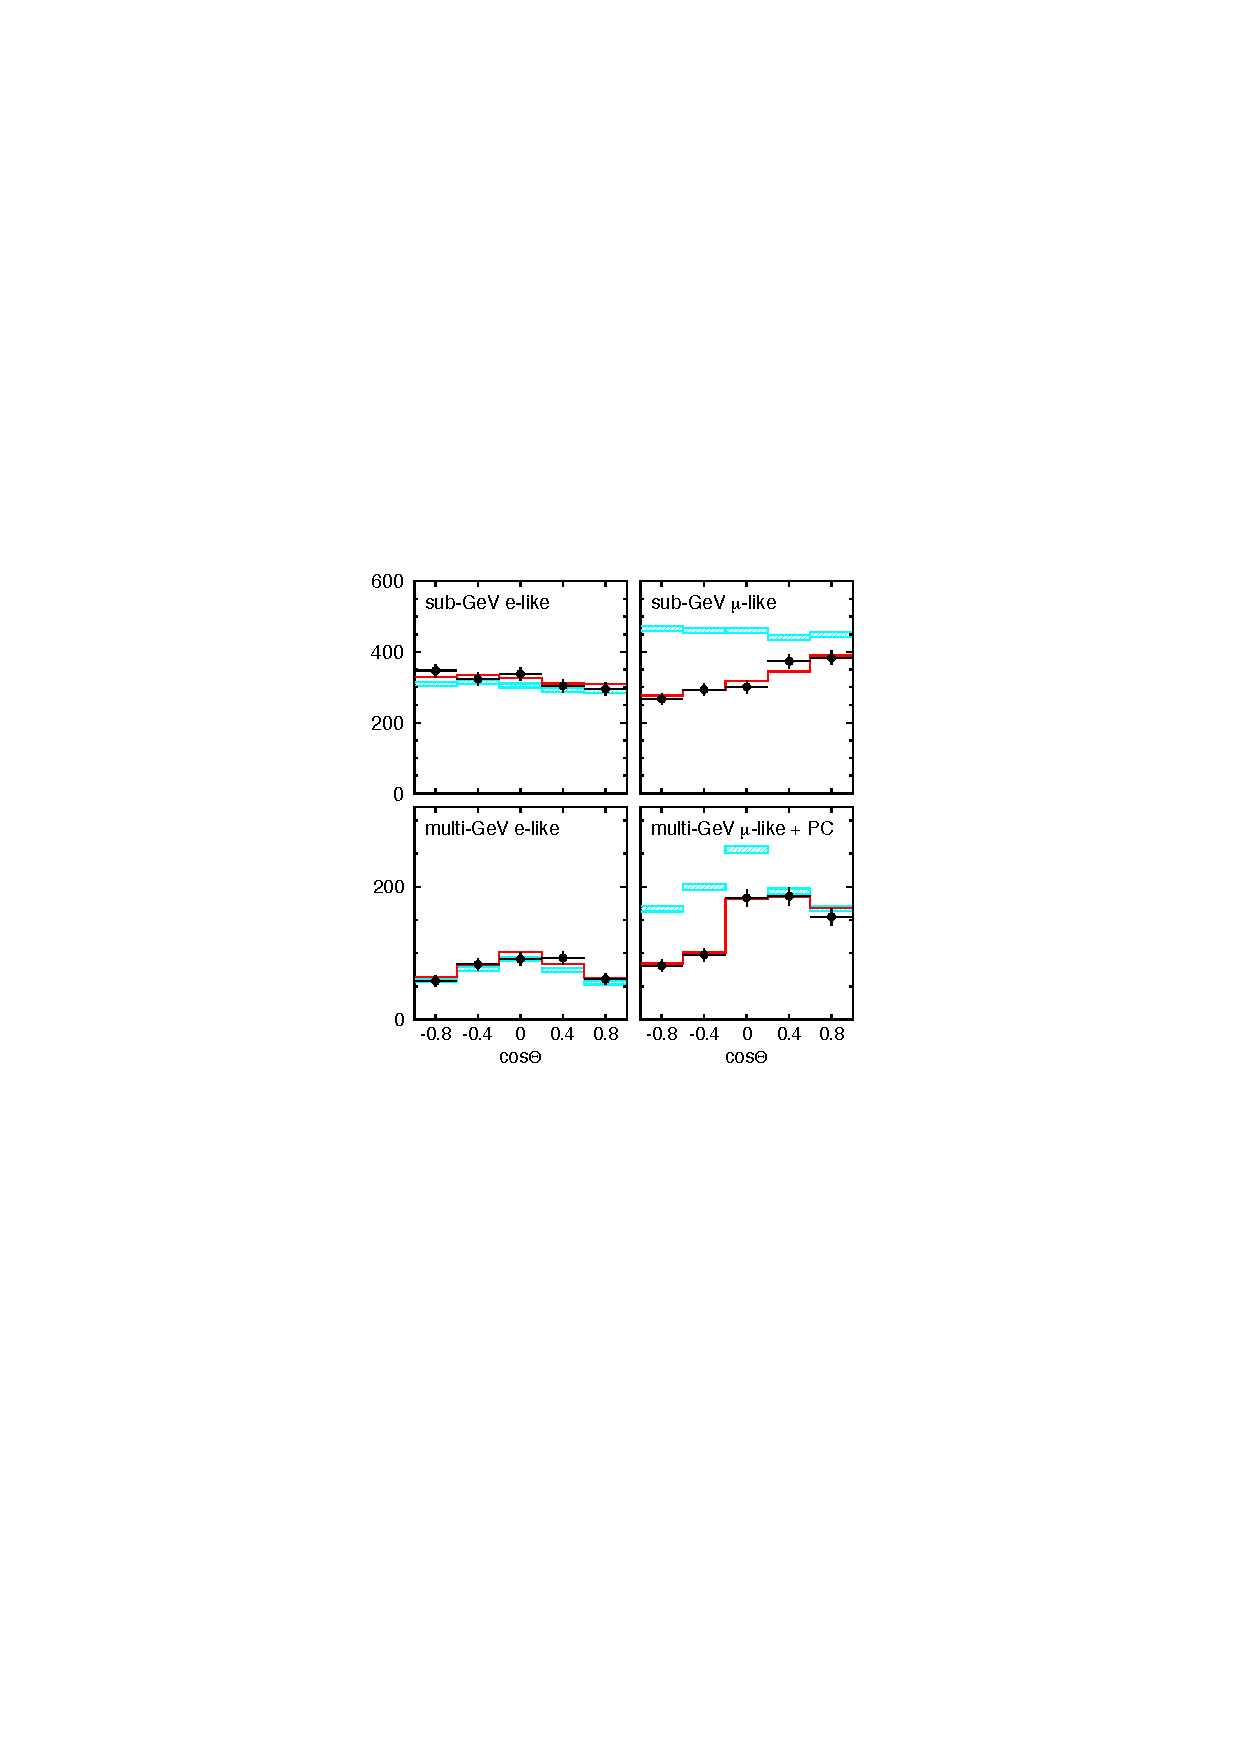
\includegraphics[height=0.4\textheight,
    width=0.4\linewidth]{./Images/SKK08}
    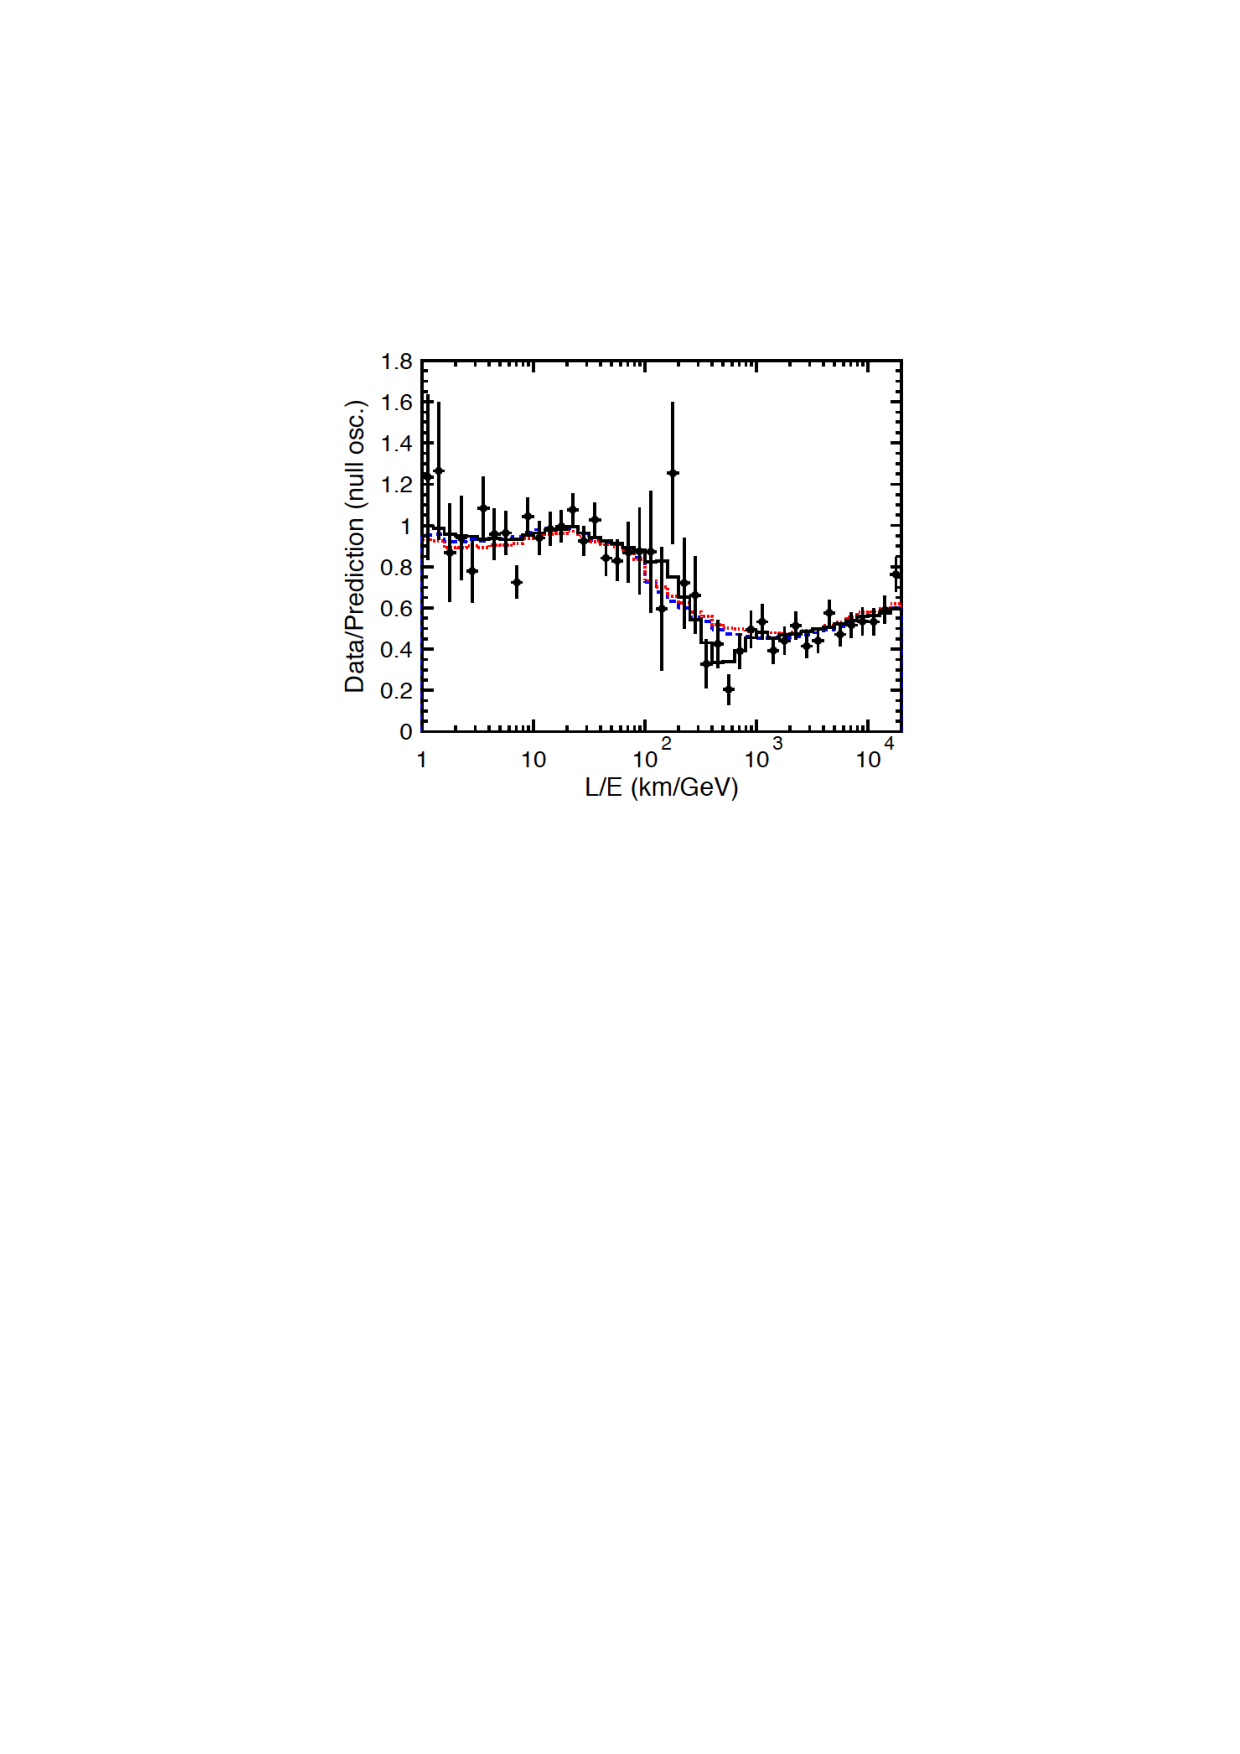
\includegraphics[height=0.4\textheight,
    width=0.4\linewidth]{./Images/SKK09}
  \end{figure}

  \note{In 1998, Super-K found first strong evidence of neutrino oscillation
  from the observation of muon neutrinos changed into tau-neutrinos
  SK has set limits on proton lifetime and other rare decays and
  neutrino properties. SK set a lower bound on protons decaying to kaons.}

\itt[<only@+>]
\item {\small left:Zenith angle distributions of $e$-like and $\mu$-like events in
  SK with momenta above $GeV$ (top) and below $GeV$ (bottom).
  The boxes show expectation assuming no oscillations.\\

  \alert{right: ratio of data from SK to Monte Carlo
  expectation assuming no oscillation, as a function of reconstructed
  $L/E$. The black histogram is a fit to a two flavour oscillation
  hypothesis.}}
\item
  whereas the flux of electron-neutrinos has almost no
  zenith angle dependence, the flux of down-going ($\cos\theta = 1$)
  muon-neutrinos significantly exceeds the flux of up-going $\nu_{\mu}$.
  \hlt{Magenta}{This can be simply interpreted in terms of neutrino oscillations}
  
  \note{neutrinos moving
    upward through the detector are created in the atmosphere at the opposite side of the Earth
    and travel thousands of kilometres before interacting. Apparently, muon-neutrinos disappear
    on the way whereas electron-neutrinos do not. Down-going muon-neutrinos, produced in the
    atmosphere directly above the detector, only travel a few dozen kilometres and are detected at
    the level expected. Since there is no indication of an increased electron-neutrino flux, the
    missing muon-neutrinos must have oscillated into tau-neutrinos.}

% \item the SK observations support the conclusion that
%   atmospheric muon-neutrinos are converted into tau-neutrinos\\
%   $-$ exclude alternative hypotheses like neutrino decay and neutrino
%   decoherence at more than $3\sigma$ (blue and red dashed lines above).
%   \alert{It also observed a tau-neutrino at almost $4\sigma$
%     level}
  \tti
\end{overlayarea}  
\end{frame}

\subsection{SNO experiment}
%%%%%% SLIDE
\begin{frame}{\textcolor{Goldenrod}{SNO experiment}}
  \begin{overlayarea}{\textwidth}{\textheight}
    % \begin{figure}[h]
    %   \centering
    % \end{figure}
    \itt[<+->]
  \item[$\Box$] \hlt{Black}{The $2 km $ underground Sudbury Neutrino Observatory (SNO,
      1999-current) has been looking for neutrinos through:}
    \[
      \begin{split}
        &\nu_{l} + e^- \to \nu_l + e^- (ES)\\
        &\nu_e + d \to e^-  + p + p (CC)\\
        & \nu_l + d \to \nu_l + n +p (NC)\\
      \end{split}
      \]
      
    \item[$\Box$] \hlt{black}{Physics aims:}\\
      $-$ \hlt{red}{solve the solar neutrino problem}\\
      $-$ neutrino oscillations\\
      $-$ information on muon neutrinos and tau neutrinos\\
      \tti 
    \end{overlayarea}    
\end{frame}


%%%%%% SLIDE
\begin{frame}{\textcolor{Goldenrod}{SNO experiment}}
  \(
  \<{0.4\textwidth}
  \img{SNO01}
  \>
  \<{0.7\textwidth}
  \itt[<+->]
  \item[\bullet] $1000$ tonnes of ultrapure heavy water
    ($99.917$\% $^2{H}$) contained within a $12 m$ diameter,
    $5.6 cm$ thick transparent acrylic vessel.\\
    \alert{{\small Highly enriched heavy
        water was required because
        $\frac{\sigma^{^1{H}}_{n-capture}} {\sigma^{^2{H}}_{n-capture}} =
        640 \to 99.85$\% enrichment}}
    
  \item[$\bullet$] $9438$ PMTs eyes on an
    $18-m$ diameter support structure. 
  \item[$\bullet$] The entire cavity outside
    the acrylic vessel was filled with ultrapure light water.
    \tti
    \>
    \)
\end{frame}

%%%%%% SLIDE
\begin{frame}{\textcolor{Goldenrod}{SNO: water system}}
  \begin{overlayarea}{\textwidth}{\textheight}
    \begin{figure}[h]
      \centering
      %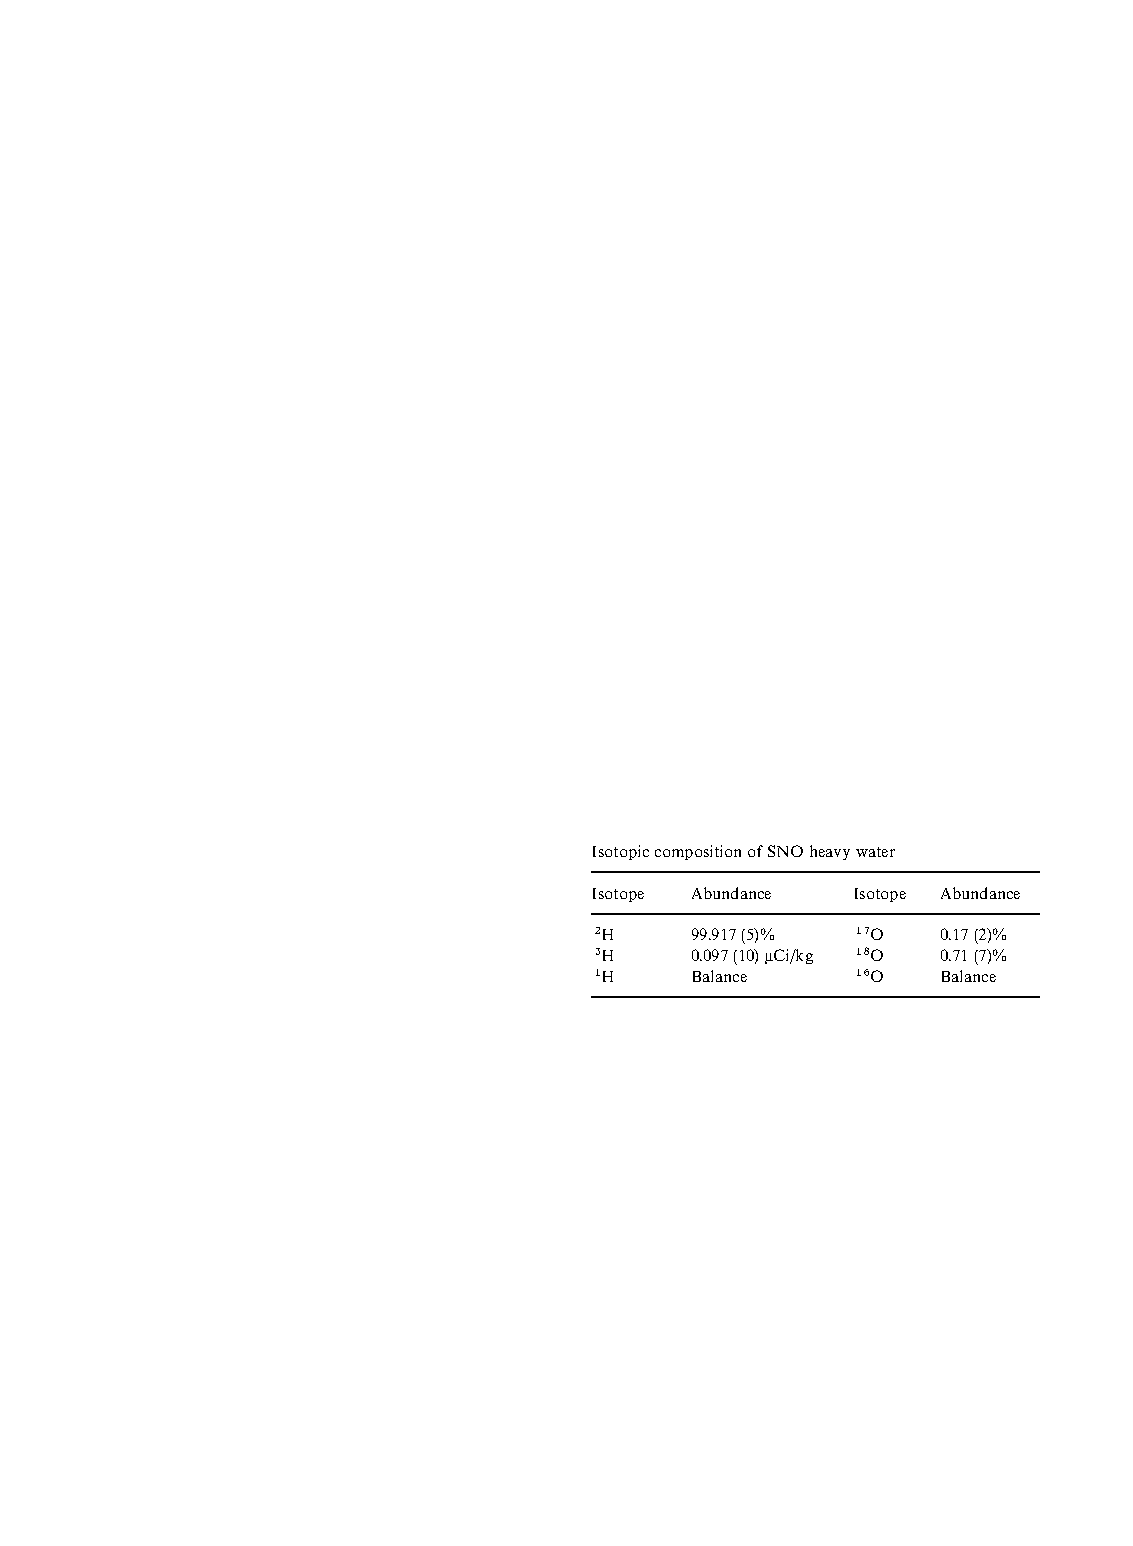
\includegraphics[height=0.25\textheight]{./Images/SNO04}\\
      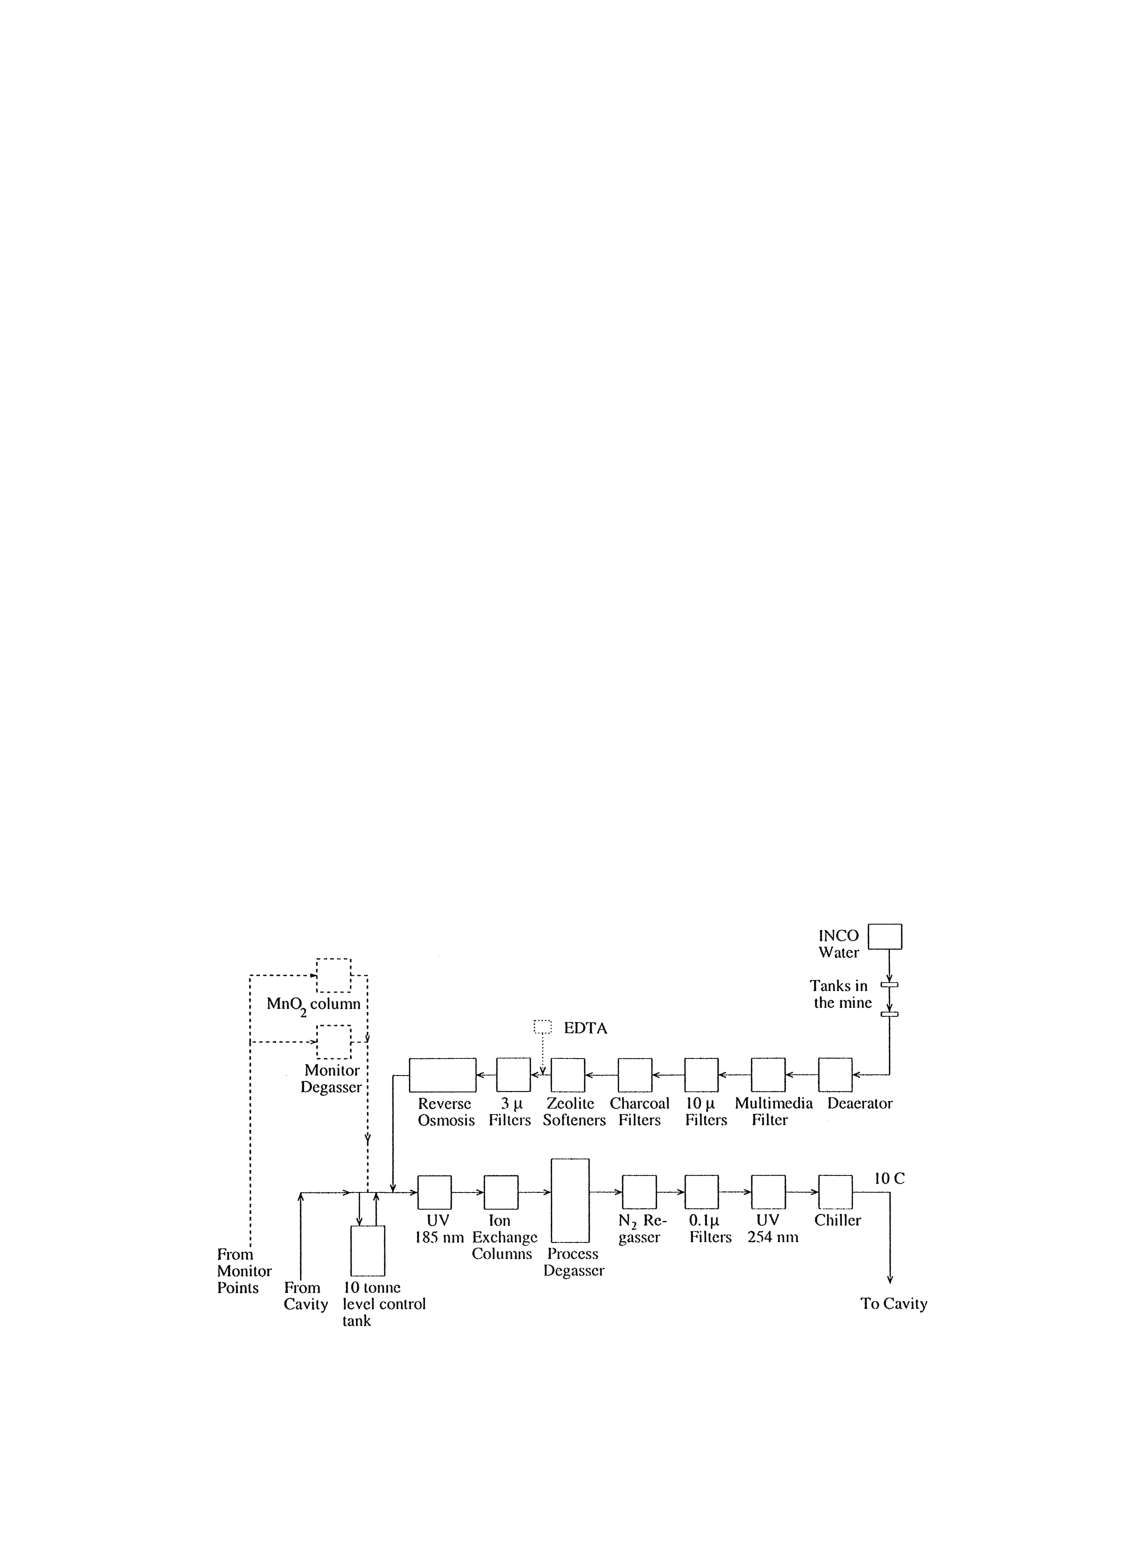
\includegraphics[height=0.3\textheight,
      width=0.48\textwidth]{./Images/SNO02}
      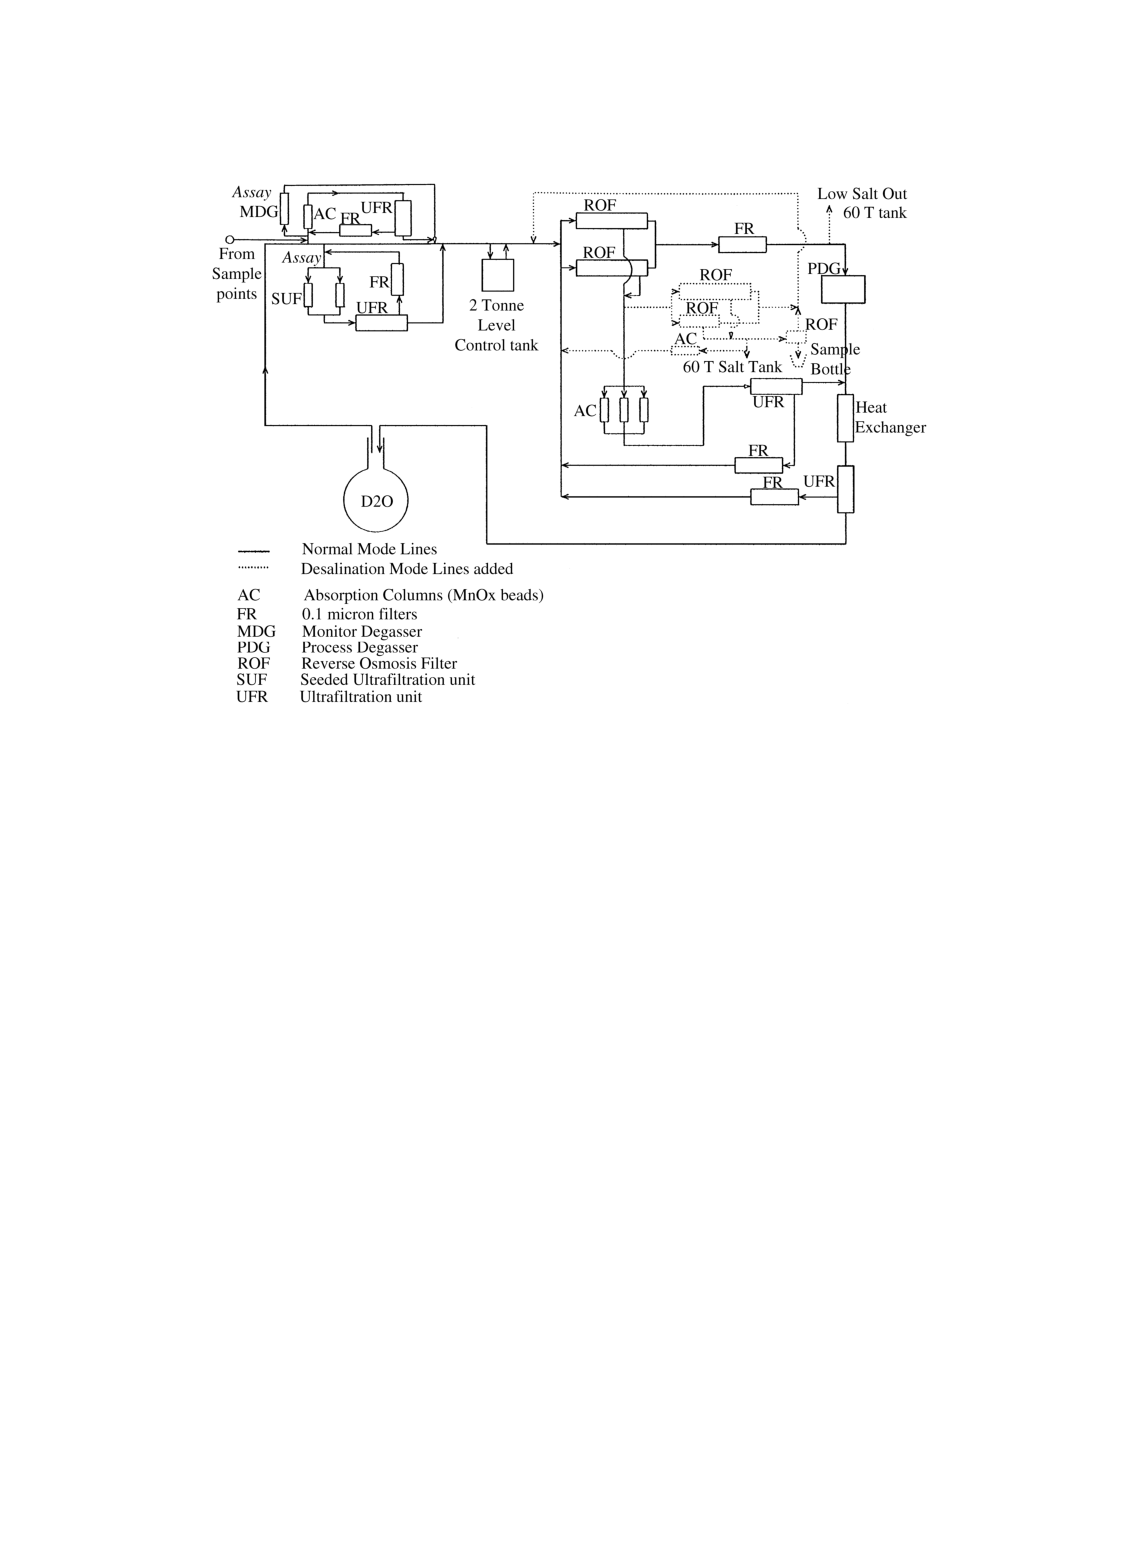
\includegraphics[height=0.3\textheight,
      width=0.48\textwidth]{./Images/SNO03}
      \caption*{left: $H_2 O$ right: $D_2 O$}
    \end{figure}
    
    \itt[<only@+>]
  \item
    two water systems at SNO: one for the ultrapure light
    water ($H_2 O$) and one for the heavy water ($D_2 O$).
    
  \item After running $H_2 O$ through a series of filtration systems,
    a degassser is used to reduce the levels of oxygen and radon, 
    then the water is cooled to $10 C$ before it goes into the cavity.\\
    \note{(not to support biological activity as well as to minimize
      radioactivity)},
    \alert{The $H_2 O$ is continuously circulated to
      remove ions, organic materials, and suspended solids.}
  \item
    The heavy water is first passed through ion-exchange columns to
    reduce its ionic content, before it goes into the acrylic vessel.\\
    \alert{{\small After the SNO detector is filled, the $D_2 O$ is recirculated to
      maintain its purity and assay it to make an accu- rate
      background determination.}}
    
  \item \textcolor{Magenta}{The $D_2 O$ and $H_2 O$ have to be isolated from the laboratory
      air to prevent radon from getting in, (A cover gas like $N_2$.)}
    
  \note{To enhance the $NC$ it's possible  add a solution 
    to the water to take advantage of the larger neutron-capture
    cross section of $Cl$ relative to deuterium.}
    \note{A concentration of approximately $0.2$\% will be used.}
    
    \note{To purify the NaCl before it was added to the heavy water for Phase
      Two, a small purification plant that included both MnOx and HTiO
      filters was built. To take the NaCl out of the water after the second
      phase of SNO running, the heavy water was passed through
      reverse-osmosis units to reduce the concentration of NaCl to a few
      parts per million.}
    \tti
    \end{overlayarea}    
\end{frame}

%%%%%% SLIDE
\begin{frame}{\textcolor{Goldenrod}{SNO: acrylic vessel}}
  \begin{overlayarea}{\textwidth}{\textheight}
    \(
    \<{0.4\textwidth}
    \img{SNO05}
    \>
    \<{0.7\textwidth}
    \hlt{black}{The primary design criteria for the containment vessel
      are:}
    \itt
  \item isolate $1000 t$ of $D_2 O$ from surrounding $H_2 O$
  \item minimize the radioactive impurities.
  \item maximize optical performance
  \item a total of $122$ ultraviolet transmitting (UVT) acrylic panels
    were used in the construction of the spherical part of the
    containment vessel. \alert{(uncompromising integrity as well as excellent
      transparency and very low radioactivity,
      ultraviolet-transmitting)}
    \tti
    \>
    \)
  \end{overlayarea}    
\end{frame}


%%%%%% SLIDE
\begin{frame}{\textcolor{Goldenrod}{SNO:  photomultiplier tubes}}
    \itt[<+->]
  \item $9438$ inward-facing PMTs, which provide a photocathode
    coverage of $31$\%. \alert{To improve the light-collection efficiency,
      a $27-cm$ entrance-diameter light concentrator is mounted on each PMT,
      increasing the effective photocathode coverage to $\approx 54$\%.}
    
  \item \hlt{Orange}{another 91 PMTs without concentrators were
      mounted facing outward to detect light from muons and other sources in
      the region exterior to the PM supporting structure.}
    \tti
\end{frame}


%%%%%% SLIDE
\begin{frame}{\textcolor{Goldenrod}{SNO: run I}}
  \begin{overlayarea}{\textwidth}{\textheight}
    \begin{figure}[h]
      \centering
      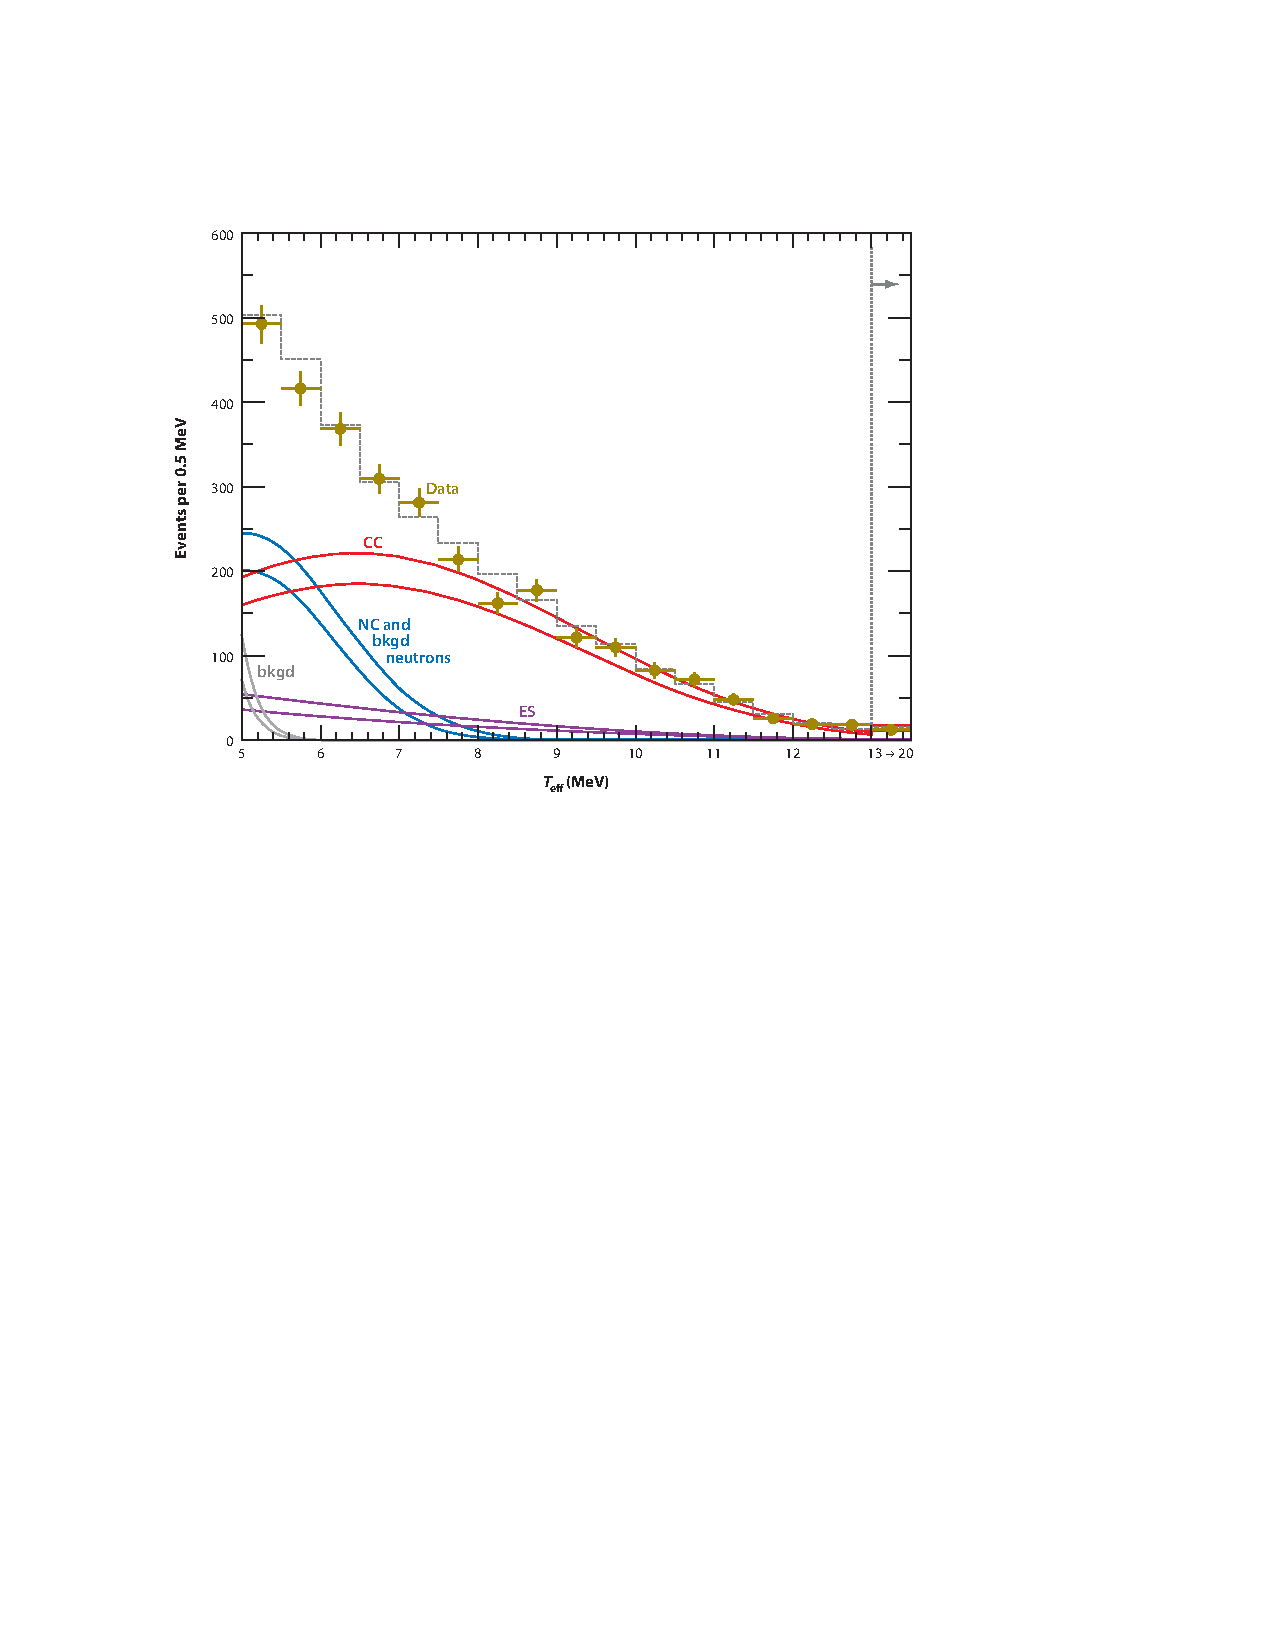
\includegraphics[height=0.20\textwidth,width=0.4\textwidth]{./Images/SNO07}
      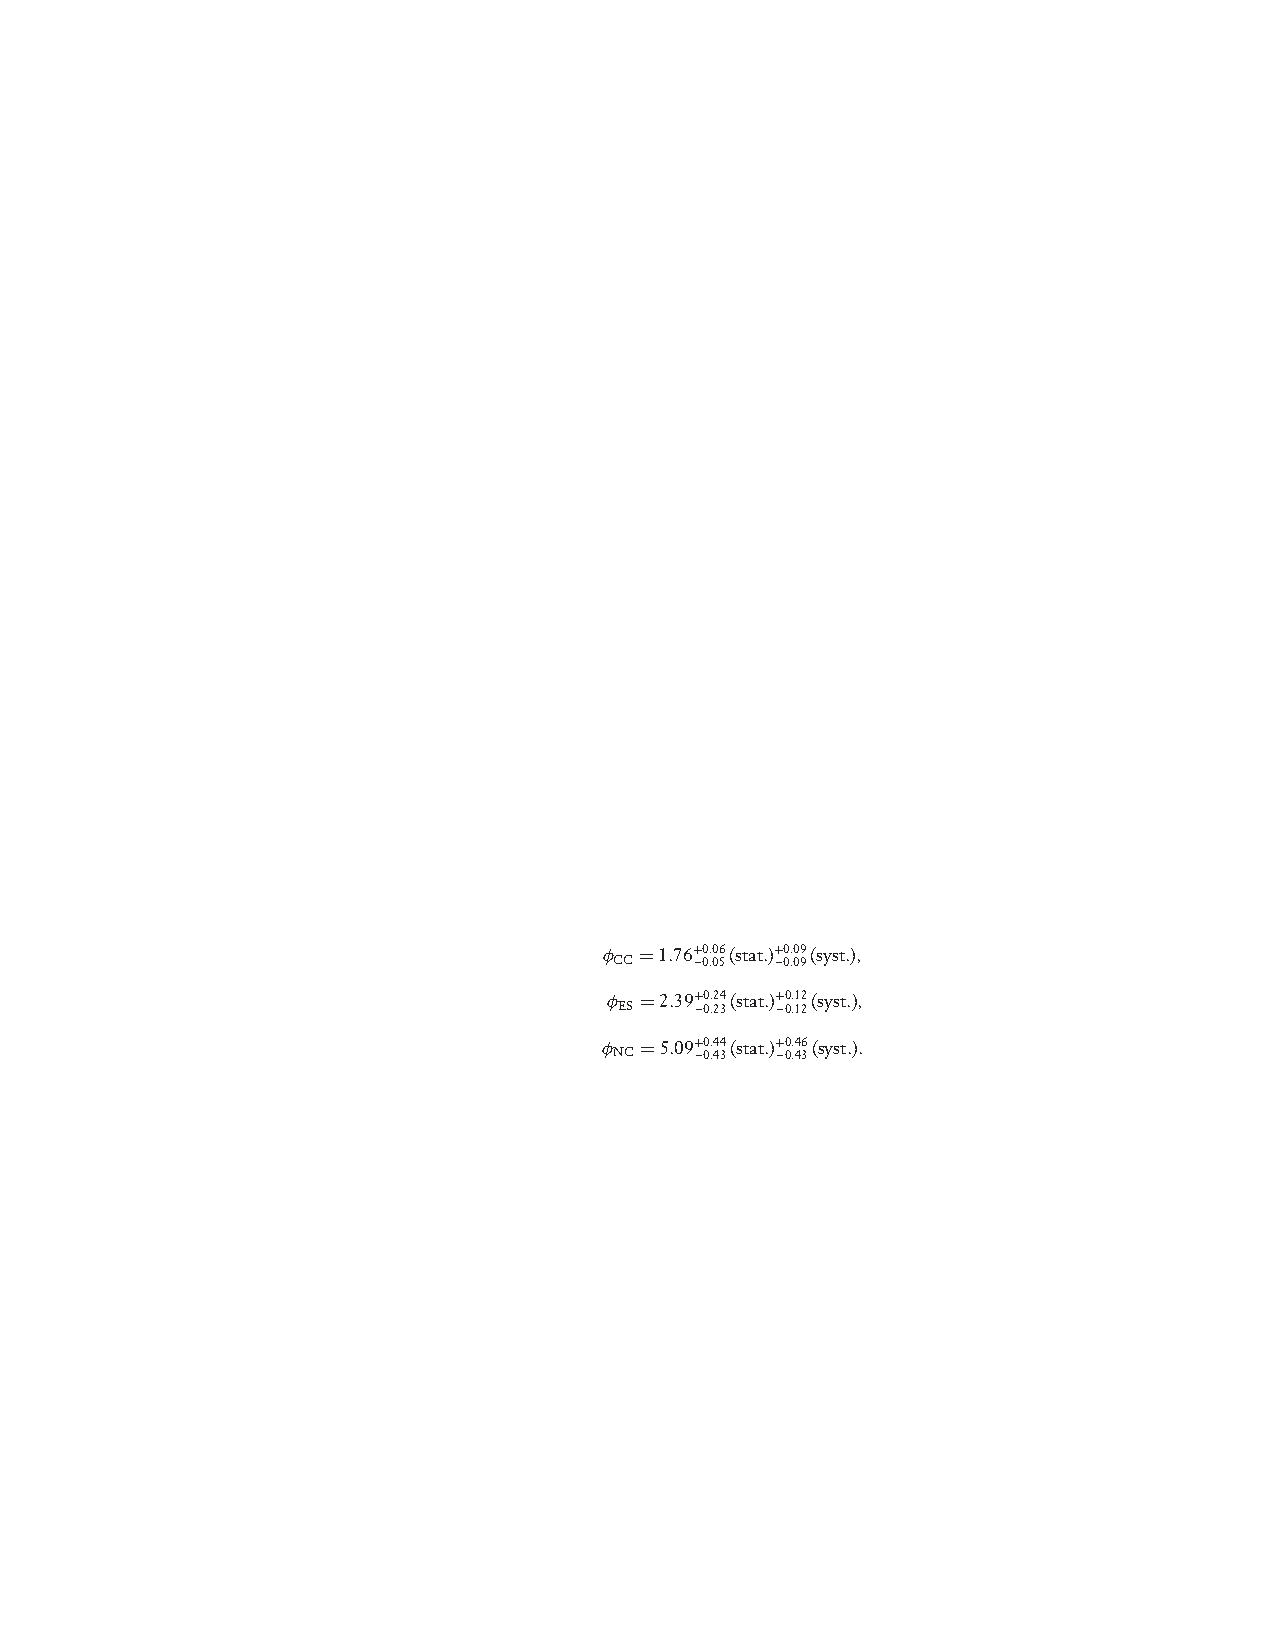
\includegraphics{./Images/SNO09}\\
      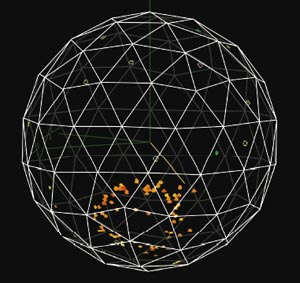
\includegraphics[height=0.15\textwidth,width=0.3\textwidth]{./Images/SNO08}
      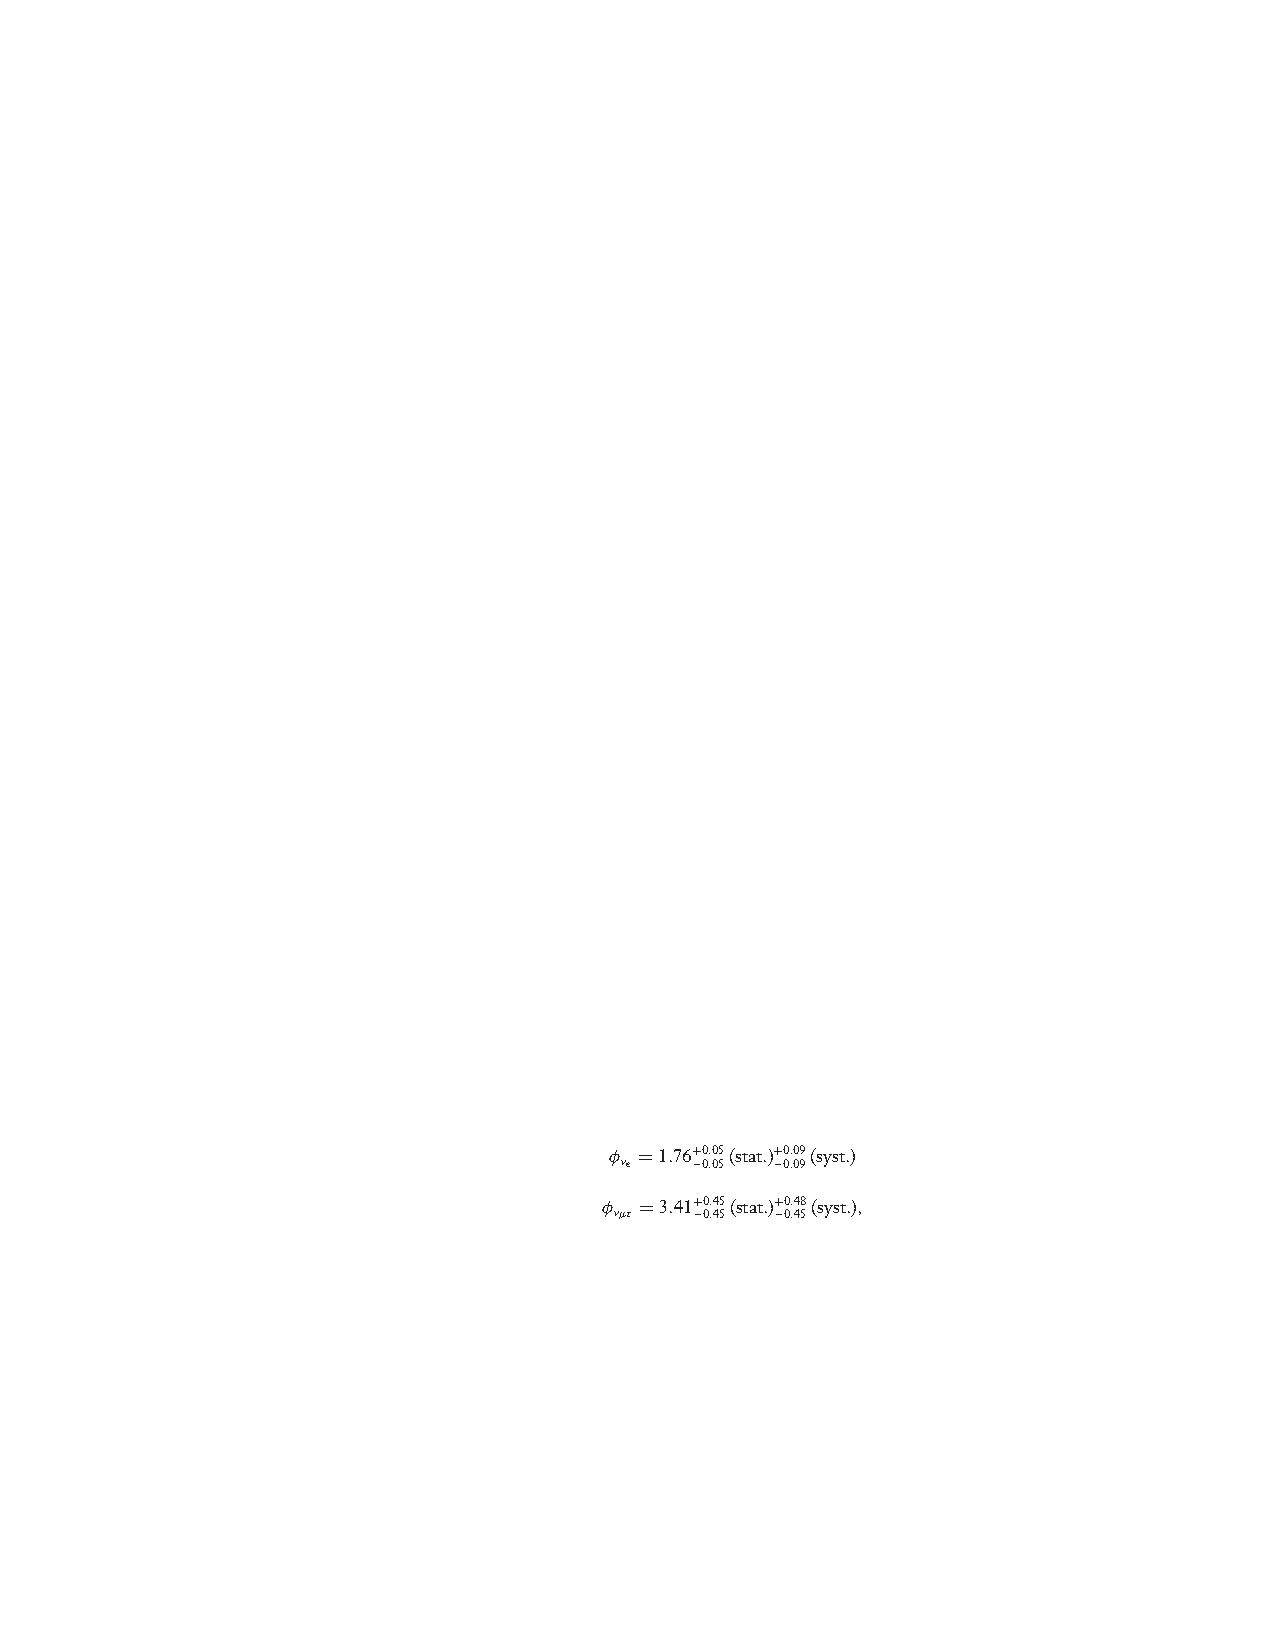
\includegraphics{./Images/SNO10}
    \end{figure}
    
    \itt[<only@+>]
  \item The first operation ($1999-2001$) using pure heavy water as
    the central detection medium.
  \item \textcolor{blue}{neutron-capture on the deuterons in $D_2 O $ releases $6.25 MeV$
      gamma rays.}\\
    $-$ \textcolor{green}{The gamma rays (Compton) scatter of the atomic electrons}\\
    $-$ \alert{the electrons above the Cherenkov threshold radiate Cherenkov light}.
  \item {\small with a $6.75 MeV$ cut on the $T_{eff}$, NC
      reaction was suppressed significantly.\\
      $-$ The $CC$ and $ES$ reactions could be resolved through use of the
      strong directional dependence of the ES reaction.\\
      \alert{neutrino flux
        are in $10^6 cm^{-2}s^{-1}$}}
    \tti
  \end{overlayarea}    
\end{frame}


%%%%%% SLIDE
\begin{frame}{\textcolor{Goldenrod}{SNO: run II}}
  \begin{overlayarea}{\textwidth}{\textheight}
    \begin{figure}[h]
      \centering
      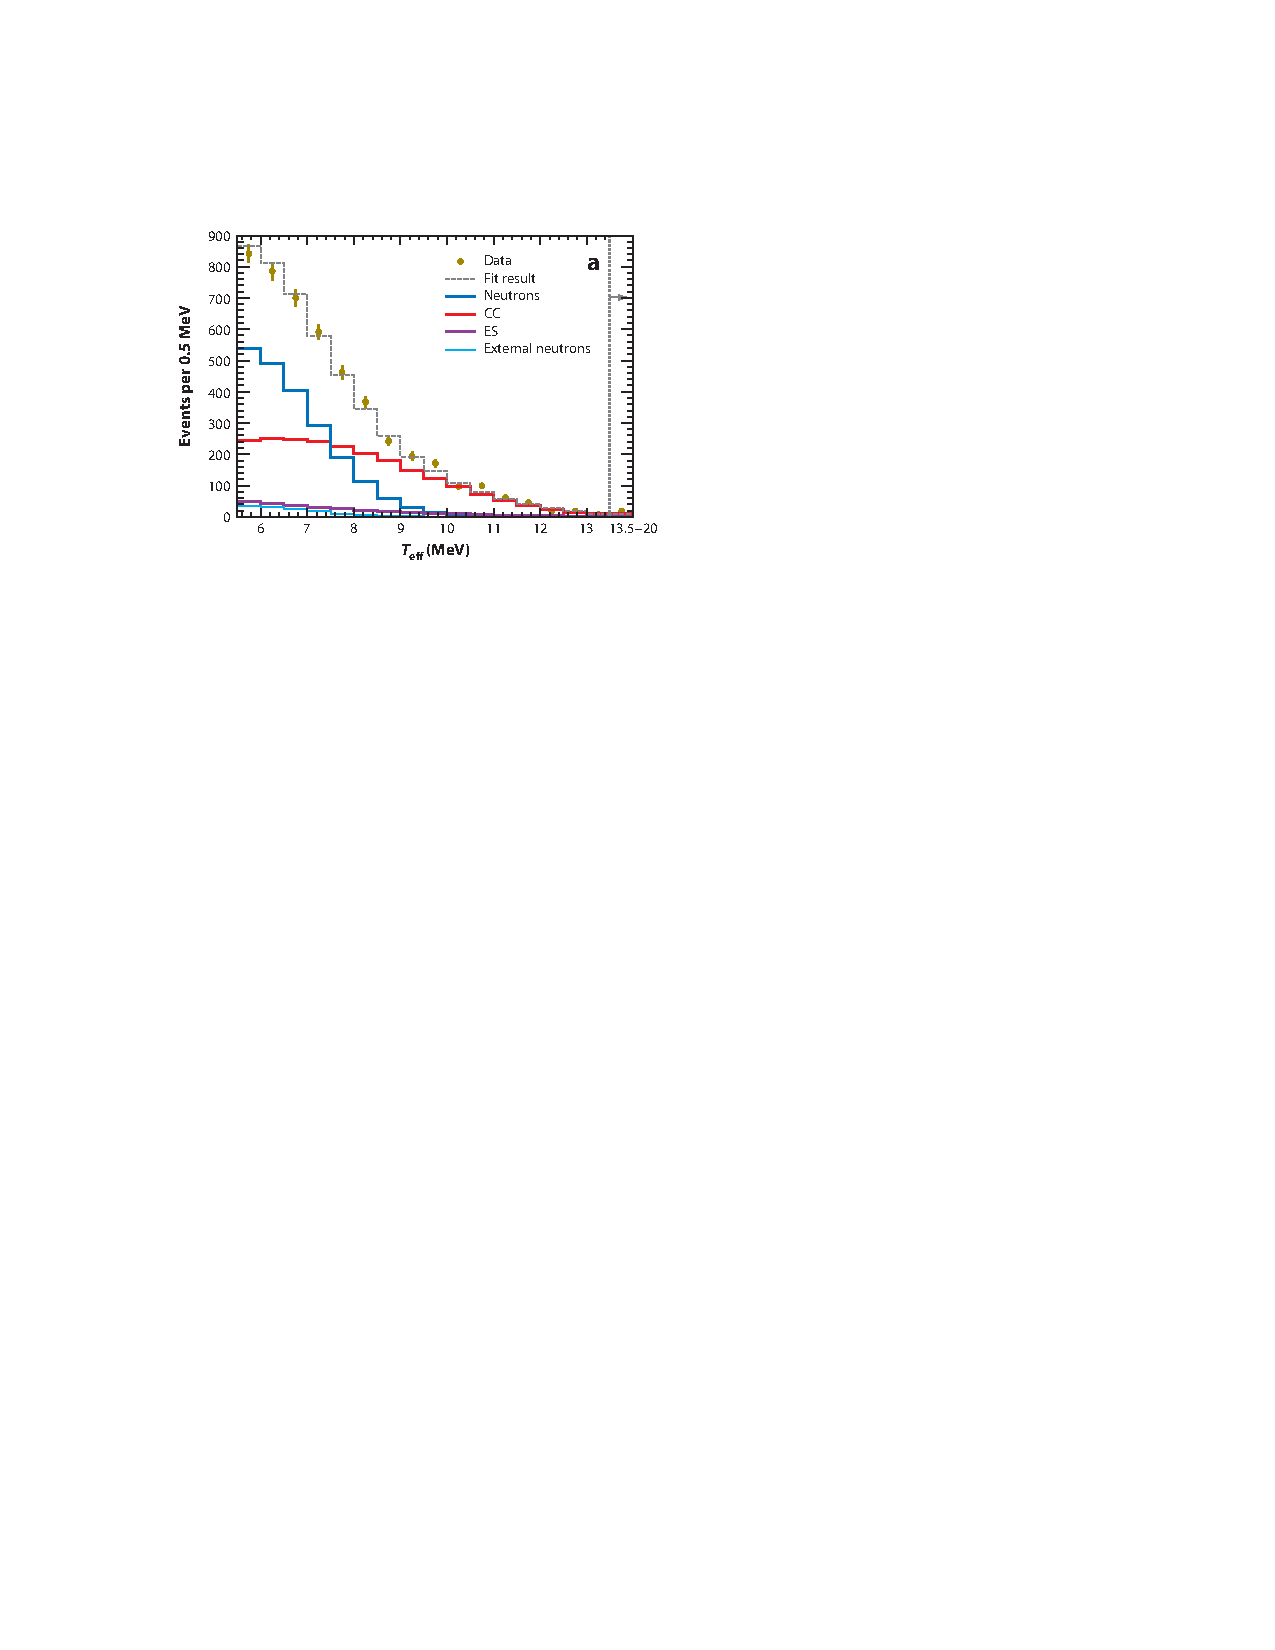
\includegraphics[height=0.2\textwidth,width=0.4\textwidth]{./Images/SNO11}
      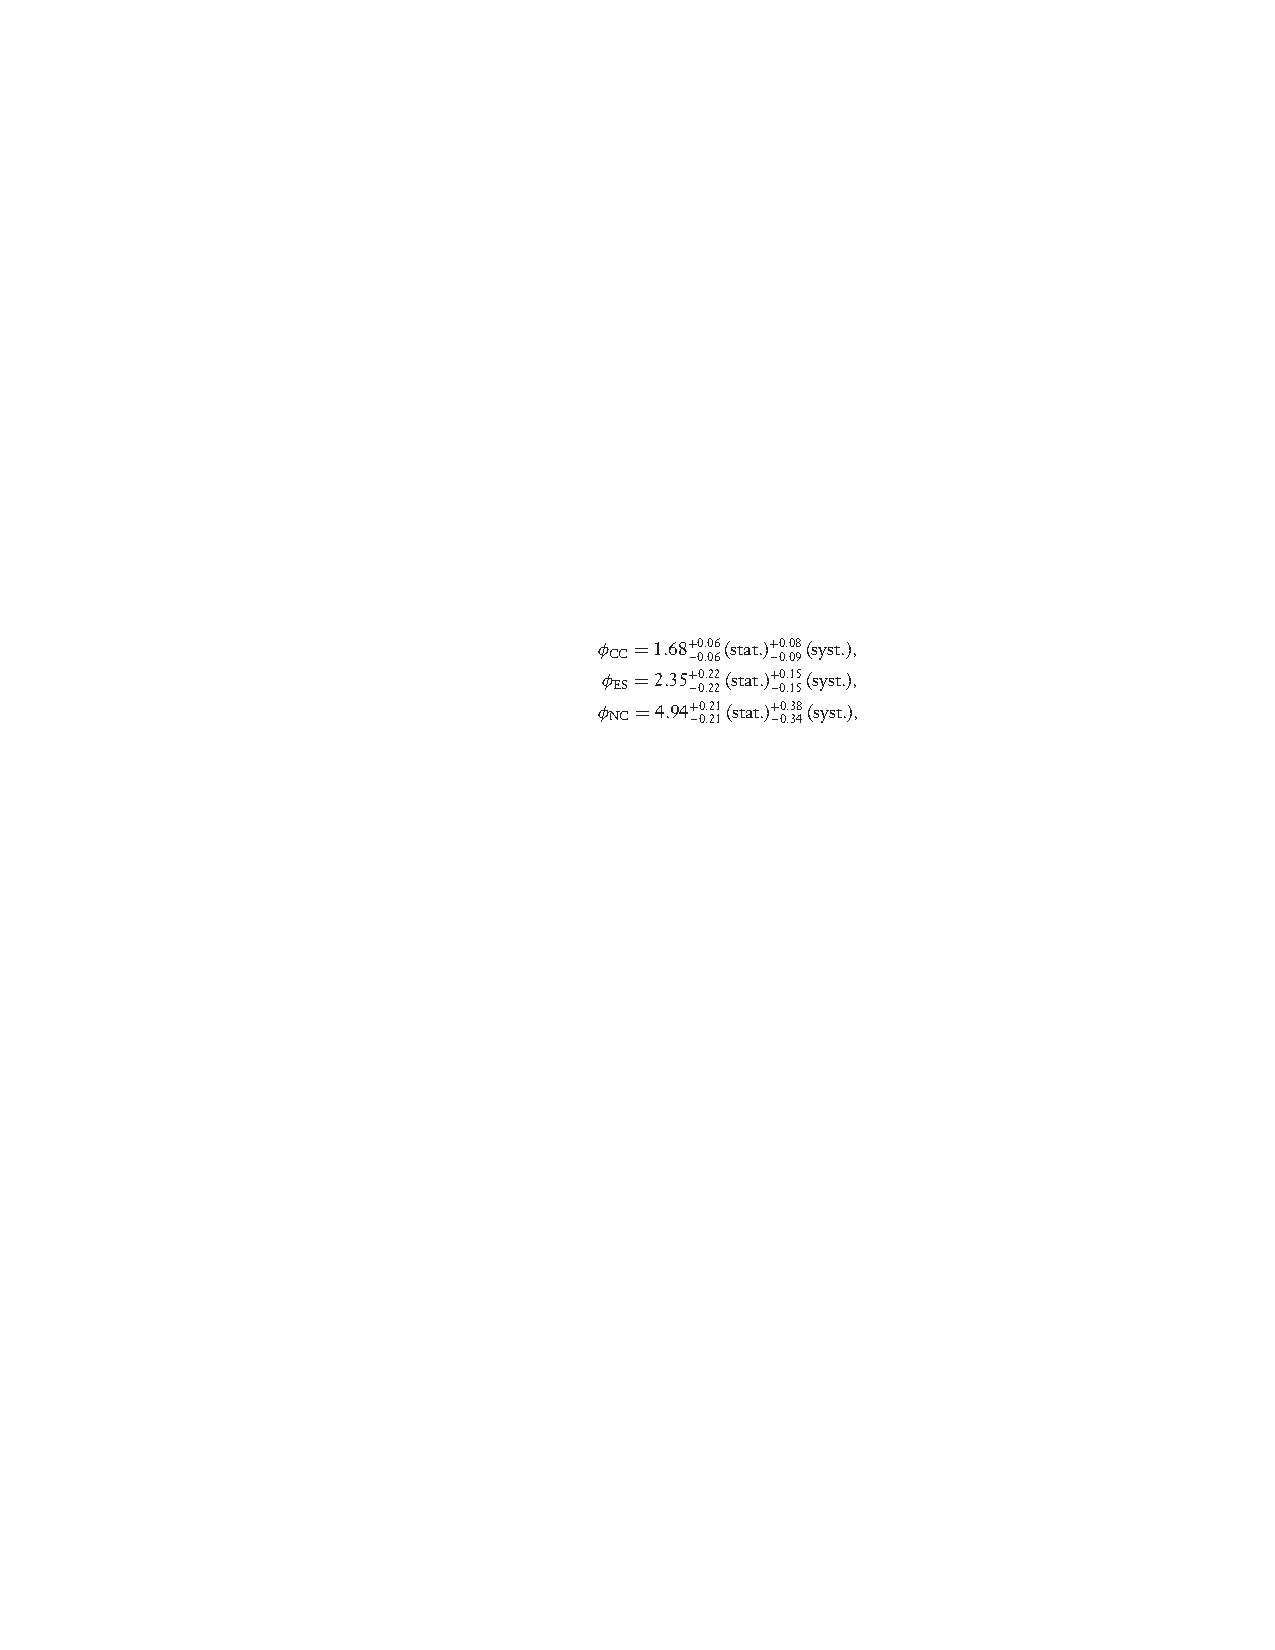
\includegraphics{./Images/SNO12}\\
    \end{figure}
    
    \itt[<only@+>]
  \item (2001-2003) salt added to $D_2 O$\\
    $1)$ the neutron-capture efficiency increases (by a factor of three)\\

    $2)$ Cherenkov light also increases because more
    energy is released in the neutron capture on $^{35}Cl$.\\
    
    $3)$ \alert{neutron capture on $^{35}Cl$ typically produces multiple
      gamma rays $\to$ multiple electrons, whereas the CC and ES reactions produce single
      electrons.}

  \item the isotropy of the Cherenkov light
    from neutron-capture events relative to CC and ES events allows
    good statistical separation 3-signals\\
    
    $\to$ \textcolor{Magenta}{
      precise measurement of the NC flux, independent of assumptions
      about the CC and ES energy spectra.}
  \tti
  \end{overlayarea}    
\end{frame}


%%%%%% SLIDE
\begin{frame}{\textcolor{Goldenrod}{SNO : run III}}
  \begin{overlayarea}{\textwidth}{\textheight}
    \begin{figure}[h]
      \centering
      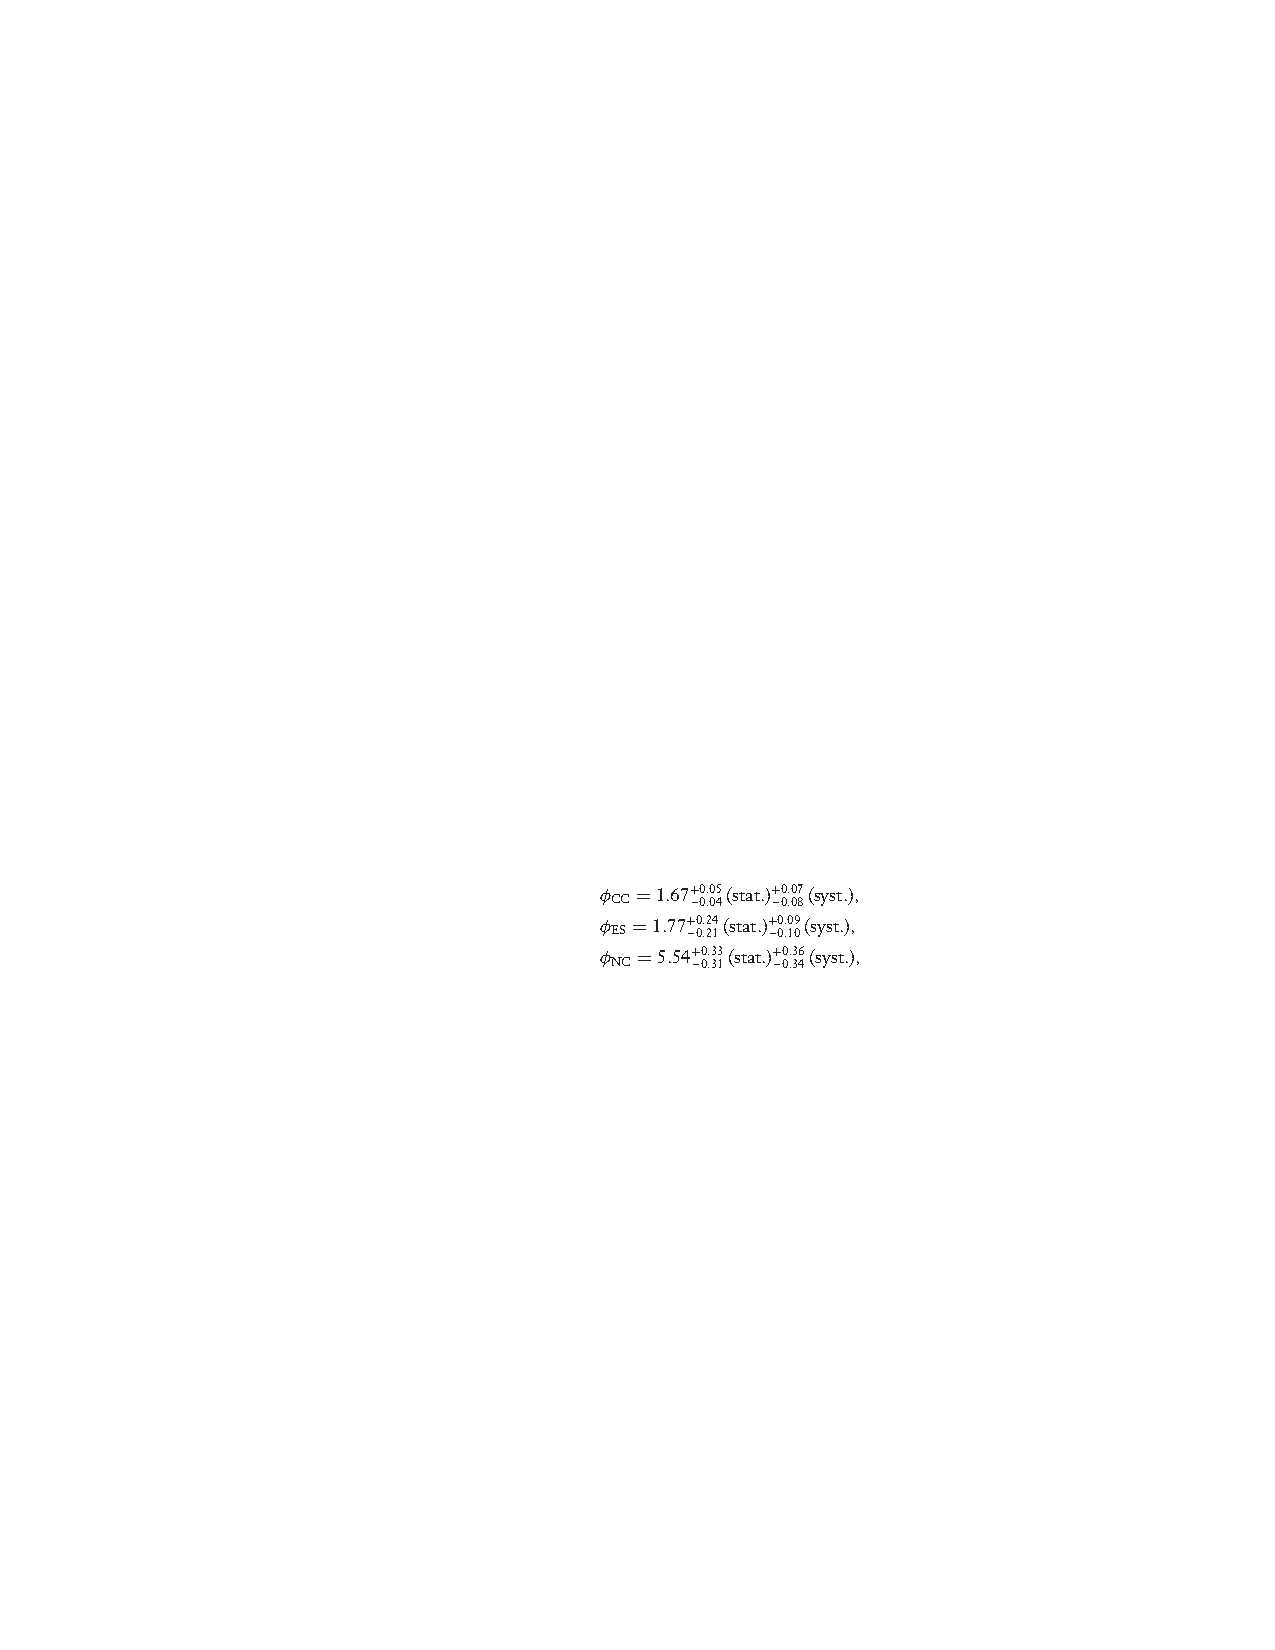
\includegraphics{./Images/SNO13}
    \end{figure}
    
    \itt[<only@+>]
  \item The extraction of the three neutrino-interaction signals from
    SNO requires breakdown of the Cherenkov light signals into the three
    components on a statistical basis.
    
    \note{Each signal has a characteristic isotropy and dependence on
      radius, angle with respect to the Sun’s position, and energy.}
    
  \item it is possible to detect the $NC$ directly through use of
    neutron-sensitive proportional counters.\\
    \alert{although neutrons do not typically cause ionization, the addition of
      a nuclide with high neutron cross-section allows the detector to
      respond to neutrons $^3{He}$, $^{6}Li$, $^{10}B$.}\\
    \hlt{black}{$^3{He} + n {\to} ^1{H}  ^3{H^+} + e^-$}
    
    \note{This different approach breaks correlations that are present
      in the Cherenkov light signals and also provides a check on possible
      systematic effects}
  \item after removing salt from $D_2 O$, an array of (40)
    proportional counters attached to anchor points on the inner surface
    filled with an $85:15$ $^3He$ and $CF_4$ inserted in the heavy water
    to detect neutrons.
    \tti
\end{overlayarea}    
\end{frame}


%%%%%%%%%%%%%% APPENDIX
% All your regular slides
% After your last numbered slide

%\appendix
\newcounter{finalframe}
\setcounter{finalframe}{\value{framenumber}}
\beginbackup
\begin{frame}[noframenumbering]
  \hlt{ForestGreen}{Additional material}
\end{frame}



%%%%%% SLIDE 
\begin{frame}{\textcolor{Goldenrod}{Neutrino-nucleon scattering}}
  \note{Coherent scattering - When you have interference between
    scattered neutron waves from different scattering centers
    (different atoms), you get information on the relative positions
    of these atoms. Thus coherent scattering gives you information on
    the relative atomic positions - structure of the material}
  
  \(
  \<{0.4\textwidth}
  \img{neutrino_nucleaon_scattering01}
  \>
  \<{0.7\textwidth}
  \hlt{black}{Coherent Elastic Neutrino-Nucleus Scattering ($CE\nu NS$):}
  \itt[<+->]
\item \alert{For a small momentum exchange $qR_N < 1$ a
    long-wavelength Z boson sees the whole nucleus.}
\item An inconspicuous low-energy nuclear recoil is the
  only observable.
\item However, the probability of neutrino interaction
  increases dramatically with the square of the number of neutrons in
  the target nucleus.
\item \alert{In scintillating materials, the ensuing dense
    cascade of secondary recoils dissipates a fraction of its energy as
    detectable light.}
  \tti
  \>
  \)
  \note{neutrino-induced neutron (NIN)}
\end{frame}

%%%%%% SLIDE 
\begin{frame}{\textcolor{Goldenrod}{Neutrino-nucleon scattering}}
  \begin{center}
    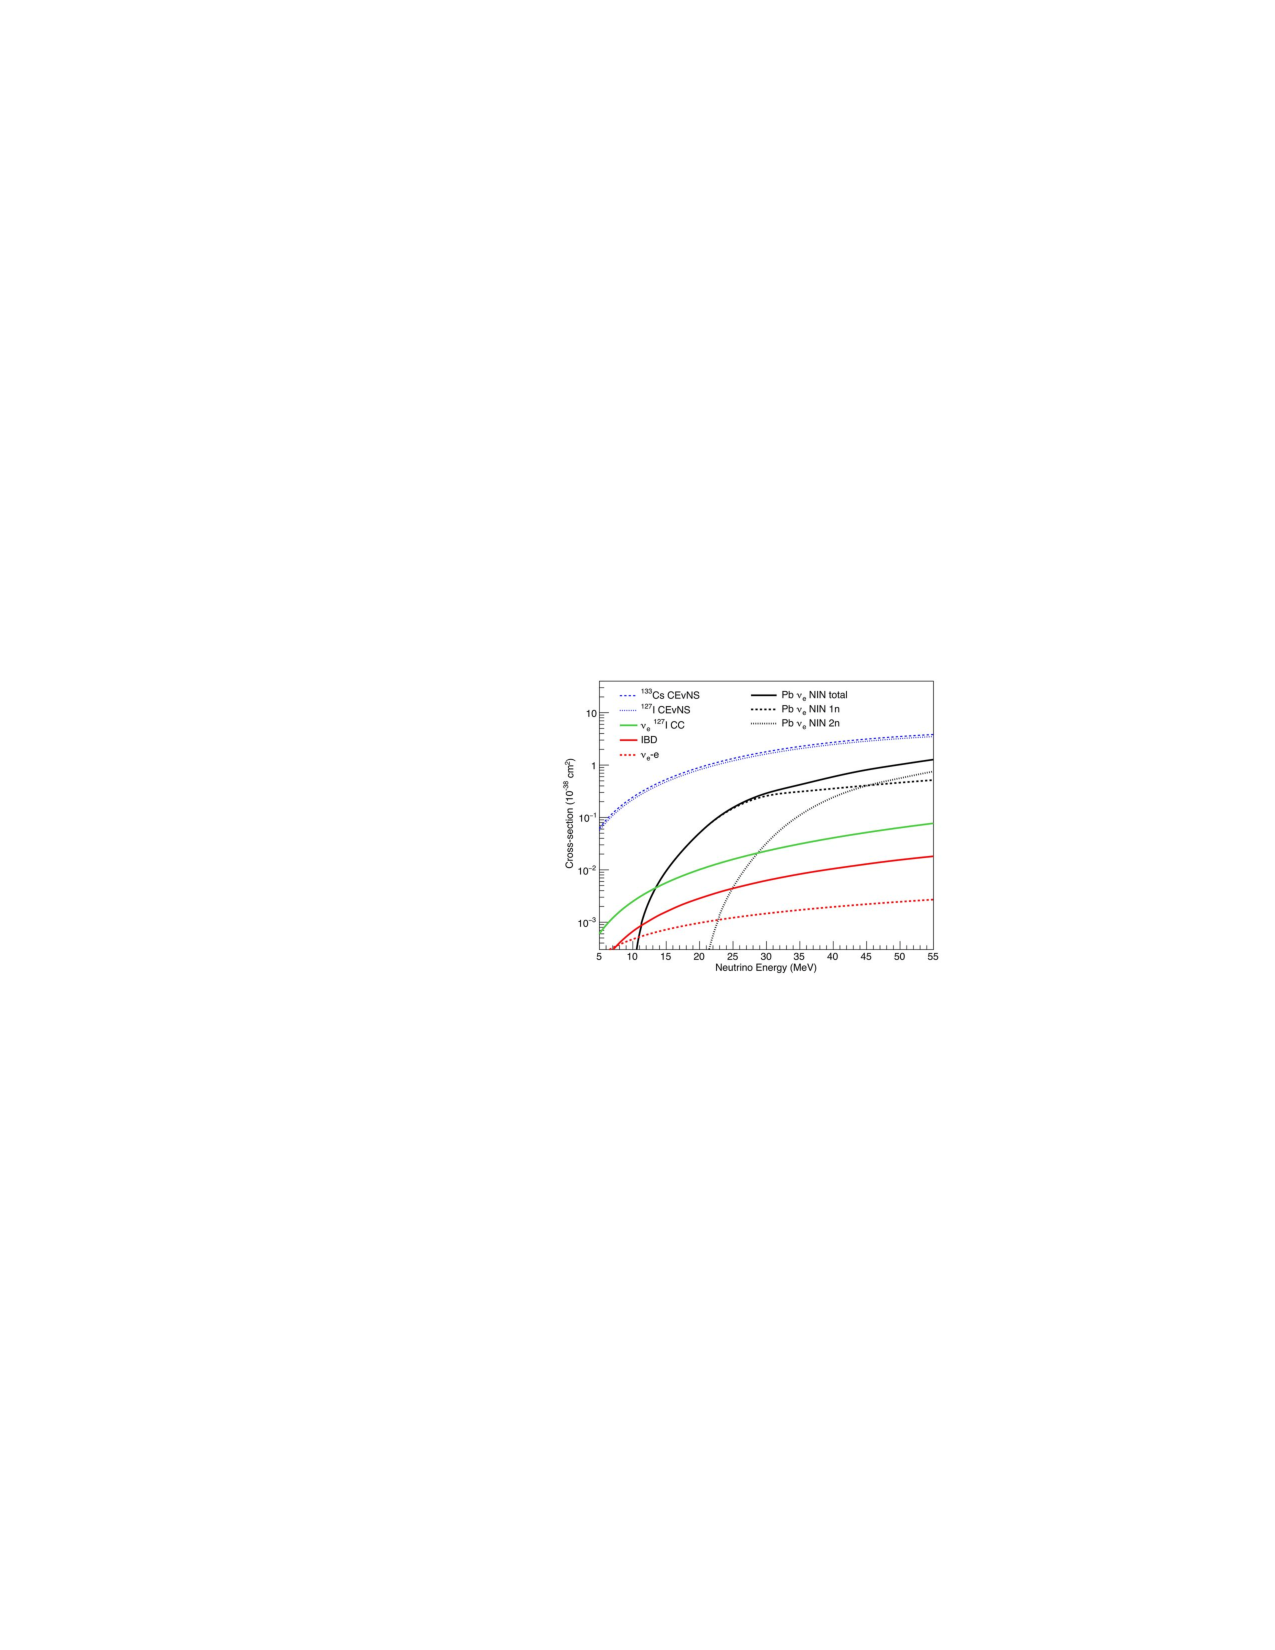
\includegraphics[height=0.4\textheight]{./Images/neutrino_nucleaon_scattering02}\\
  \end{center}
  \hlt{Green}{Total cross-sections from $CE\nu NS$ and some known
    neutrino couplings.}
  \itt[<+->]
  \note{included are neutrino-electron scattering, charged-current (CC)
    interaction with iodine, and inverse beta decay (IBD).}
\item because of their similar nuclear masses, cesium and iodine
  respond to $CE\nu NS$ almost identically.
\item \alert{the present $CE\nu NS$ measurement involves neutrino energies in
    the range $ 16-53 MeV$}
  \note{the lower bound defined by the lowest nuclear
    recoil energy measured, the upper bound by SNS(Spallation Neutron Source) neutrino
    emissions.}\\
  \note{The cross-section for neutrino-induced neutron (NIN) generation
    following $^{208}Pb(\nu_e,e^- xn)$ is also shown. This reaction,
    originating in lead shielding around the detectors, can generate a
    potential beam-related background affecting $CE\nu NS$ searches. The
    cross-section for $CE\nu NS$ is more than two orders of magnitude
    larger than for IBD, the mechanism employed for neutrino discovery.}
  \tti
\end{frame}


%%%%%% SLIDE 
\begin{frame}{\textcolor{Goldenrod}{Homestake experiment}}
  \begin{overlayarea}{\textwidth}{\textheight}
    \begin{figure}[h]
      \centering 
      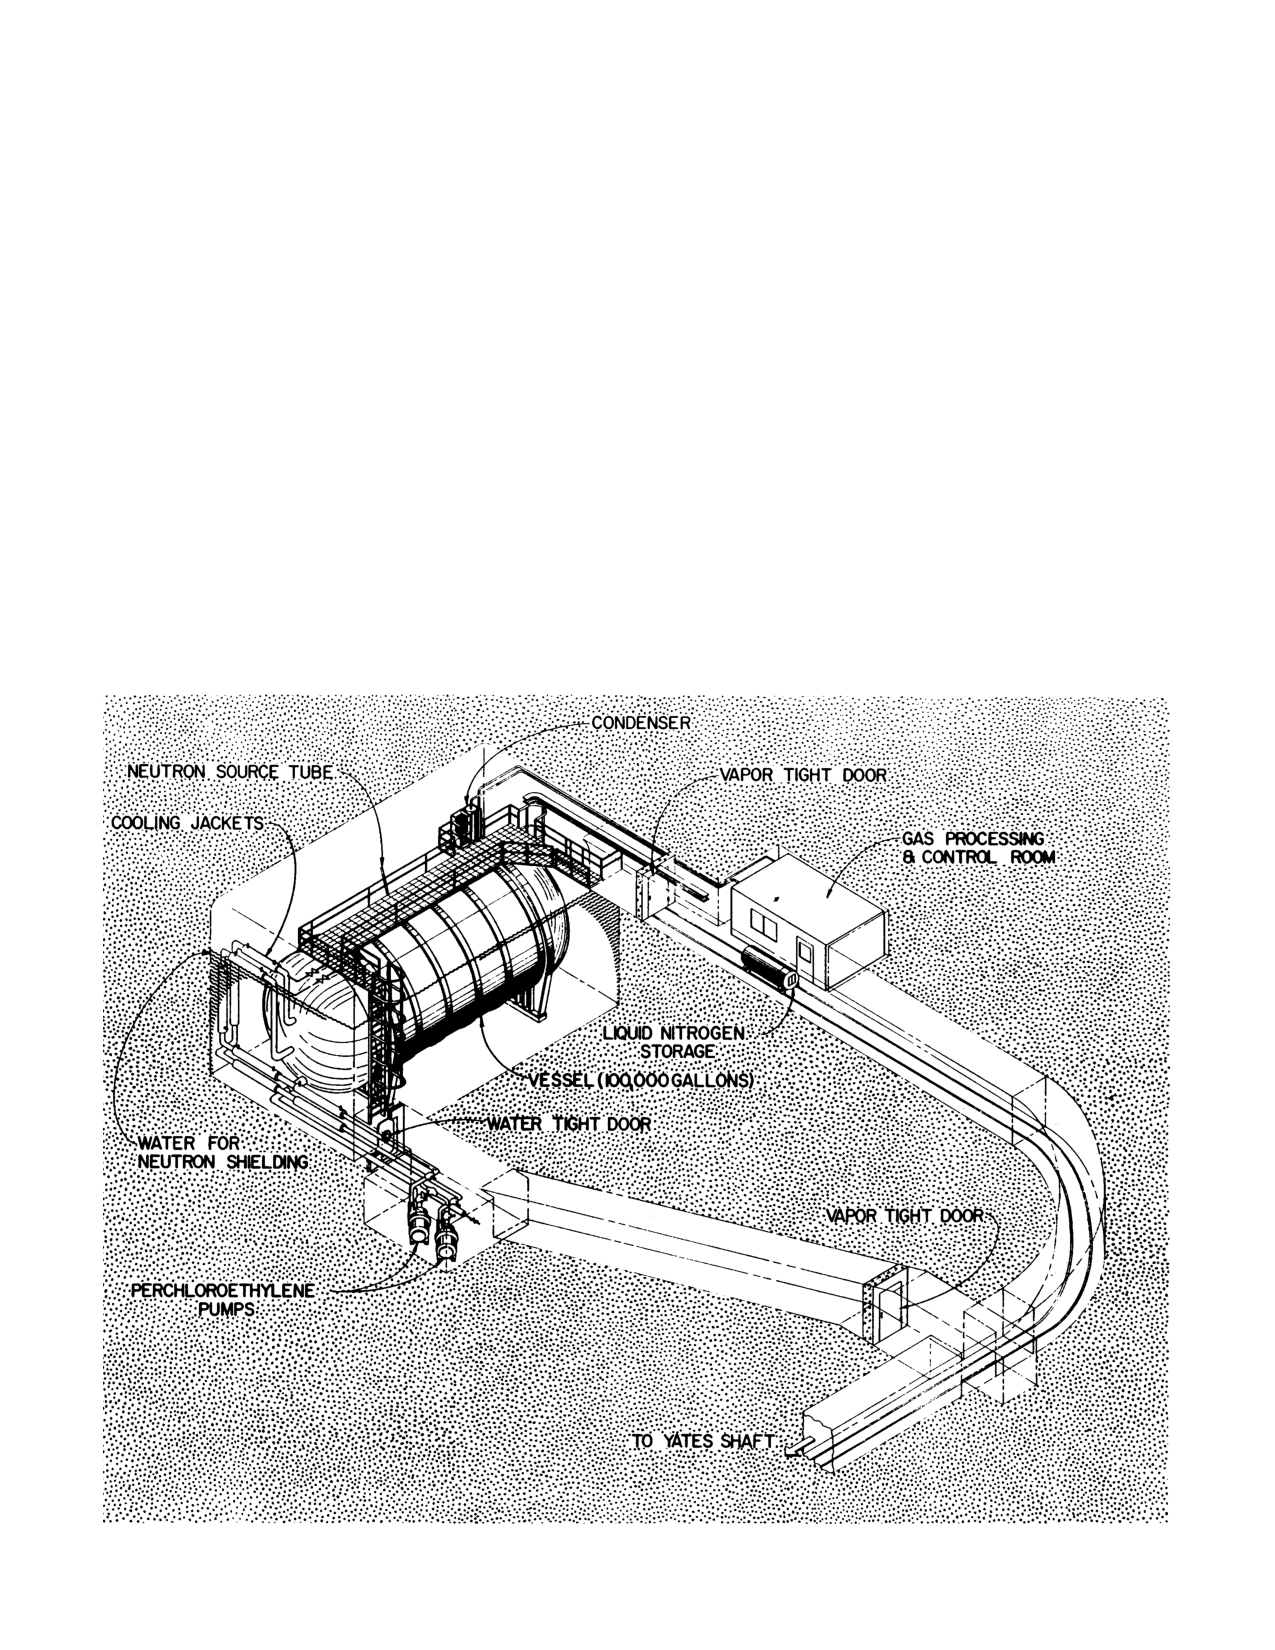
\includegraphics[width=0.7\textwidth, height=0.4\textheight]{./Images/HomeStake01}
    \end{figure}
    \itt[<only@+>]
  \item The apparatus consists of a single horizontal steel tank with
    dished ends, $6.1 m$ in diameter and $14.6 m$ long, containing $615$
    metric tons of tetrachloroethylene, $C_2Cl_4$ .
    \note{The tetrachloroethylene fills about 95\% of the detector volume
  with the remaining 5\% filled with helium gas at 1.5 atm pressure
  (absolute). The tank is set below the entrance adit so that the cavity
  can be ooded with water to shield the detector from fast neutrons
  from the rock wall.}

\item \hlt{RoyalBlue}{solar neutrinos convert a very small number of the
    $^{37}Cl$ atoms into $^{37}Ar \to$ the challenge is to remove
    these $^{37}Ar$ atoms efficiently from the detector and determine
    their number.}
  
  \note{Because the 37Ar atoms begin to decay back to 37Cl within the
    tank even as they are created, the total number of 37Ar atoms in the
    tank grows only to a saturation level where the production rate is
    equal to the decay rate}
  \note{Since argon is a light noble gas, it will not chemically or
    physically (van der Waals) attach to tetrachloroethylene.}
  \note{Dissolved argon is easily removed from the C2Cl4 by purging
    the liquid with helium. The argon then can be removed from the helium
    gas stream with a suitable absorber. Finally, the argon sample is
    chemically purified and inserted into a small proportional counter to
    determine the number of 37Ar atoms recovered.}

\item The system for removing the argon from the tank involves two
  steps:\\ $1)$ {\small maintaining an equilibrium between the $Ar_{gas}$ and
    $Ar_{disolved}$ by bubbling helium through the tank}\\ $2)$ \small{
    sweeping the helium atmosphere of the tank through an external,
    cryogenically cooled absorber that traps the argon but allows the
    helium to pass through and return to the detector.}

  \note{As the argon in the
    gas reservoir is depleted due to adsorption onto the absorber, the
    liquid- gas mixing process restores equilibrium by transferring
    additional argon from the detector liquid to the gas.}

\item \hlt{Red}{The Homestake detector observed less than $1/3 SNU$
    (One solar neutrino unit $=$ one interaction per $10^{36}$ target atoms
    $s^{-1}$.) than it expected}
  \tti
\end{overlayarea}
\end{frame}


%\subsection{CDHS experiment}
%%%%%% SLIDE
\begin{frame}{\textcolor{Goldenrod}{The CDHS}}
  \begin{overlayarea}{\textwidth}{\textheight}
  \begin{figure}[h]
    \centering
    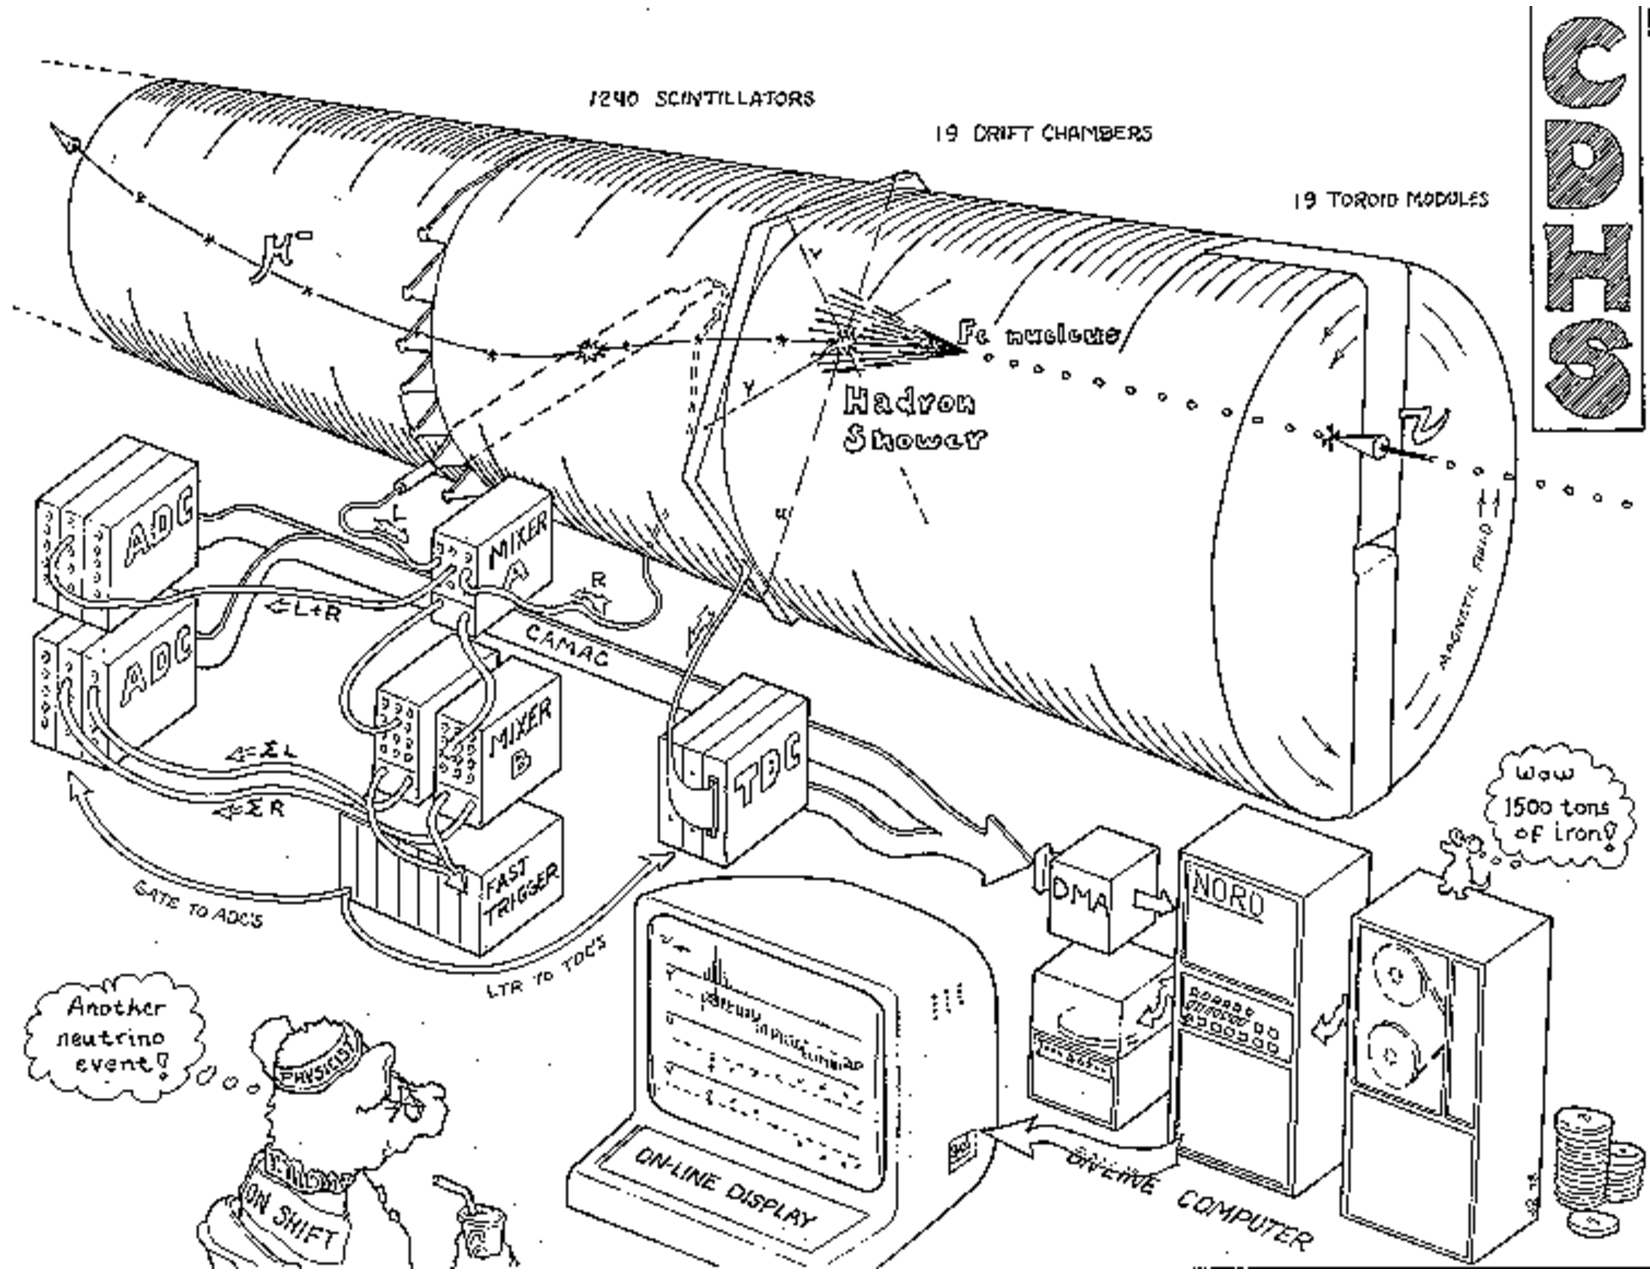
\includegraphics[height=0.4\textheight, width=0.8\linewidth]{./Images/cdhscomicb.pdf}
  \end{figure}
  \note{The CDHS neutrino experiment at CERN was a collaboration of CERN,
    Dortmund, Heidelberg and Saclay (later joined by Warsaw) led by Jack
    Steinberger.}
  
  \note{The experiment took data in
    the CERN neutrino beams from December 1976 until 1984}.
  
  \itt[<only@+>]
\item \hlt{SeaGreen}{probing deep inelastic neutrino interactions in
    iron.}
  \[
    \begin{aligned} &\nu_{\mu} + Fe \to \nu_{\mu} + X (NC)\\
      &\nu_{\mu} + Fe \to \mu + X (CC)\\
    \end{aligned}
  \]
\item {\small The detector is a magnetized iron cylinder ($3.85 m$ in
    diameter and mass of $1250 tons$) and combined the functions of a muon
    spectrometer and hadron calorimeter. \alert{It consisted of 19
      magnetized iron modules ($0.75m$), separated from each other by
      scintillators and wire drift chambers.}}
\item drift chambers are inserted between the modules for muon
  tracking. The scintillator structure allows one to measure the
  position of the shower
  \tti
  \note{Later, a $31 m^3$ liquid
    hydrogen tank was placed in front of the experiment to study neutrino
    interactions in hydrogen.}
\end{overlayarea}
\end{frame}  

%%%%%% SLIDE 
\begin{frame}{\textcolor{Goldenrod}{The CDHS}}

  \note{The main idea of the experiment is to measure
    only the hadronic showers produced in neutrino interactions, in
    order to treat NC and CC interactions alike, as much as possible. In
    particular, no pattern recognition or track reconstruction for muons
    of CC events is performed. In this way, when forming the ratio of NC
    events to CC events, many sources of systematical errors are eliminated.}
  
  \(
  \<{0.75\textwidth}
\itt
\item<1-> The detector records neutrino-iron interactions producing
  hadronic showers of energies above the trigger threshold of about $3
  GeV$.
\item<2-> \alert{If the active elements in a total-absorption or sampling calorimetric
    system provide some spatial information, one is able to distinguish
    different final-state products in such neutrino tracking detectors.}
\item<3-> \hlt{Orange}{a di-muon event in the CDHS detector.}
  \note{In this
    event reconstruction the energy deposits and the muon tracks in
    different projections are shown.}
  \tti
  \>
  \onslide<3->
  \<{0.45\textwidth}
  \img{CDHS02}
  \>
  \)
\end{frame}

%%%%%% SLIDE
% \begin{frame}{\textcolor{Goldenrod}{The CDHS}}
%   \begin{center}
%     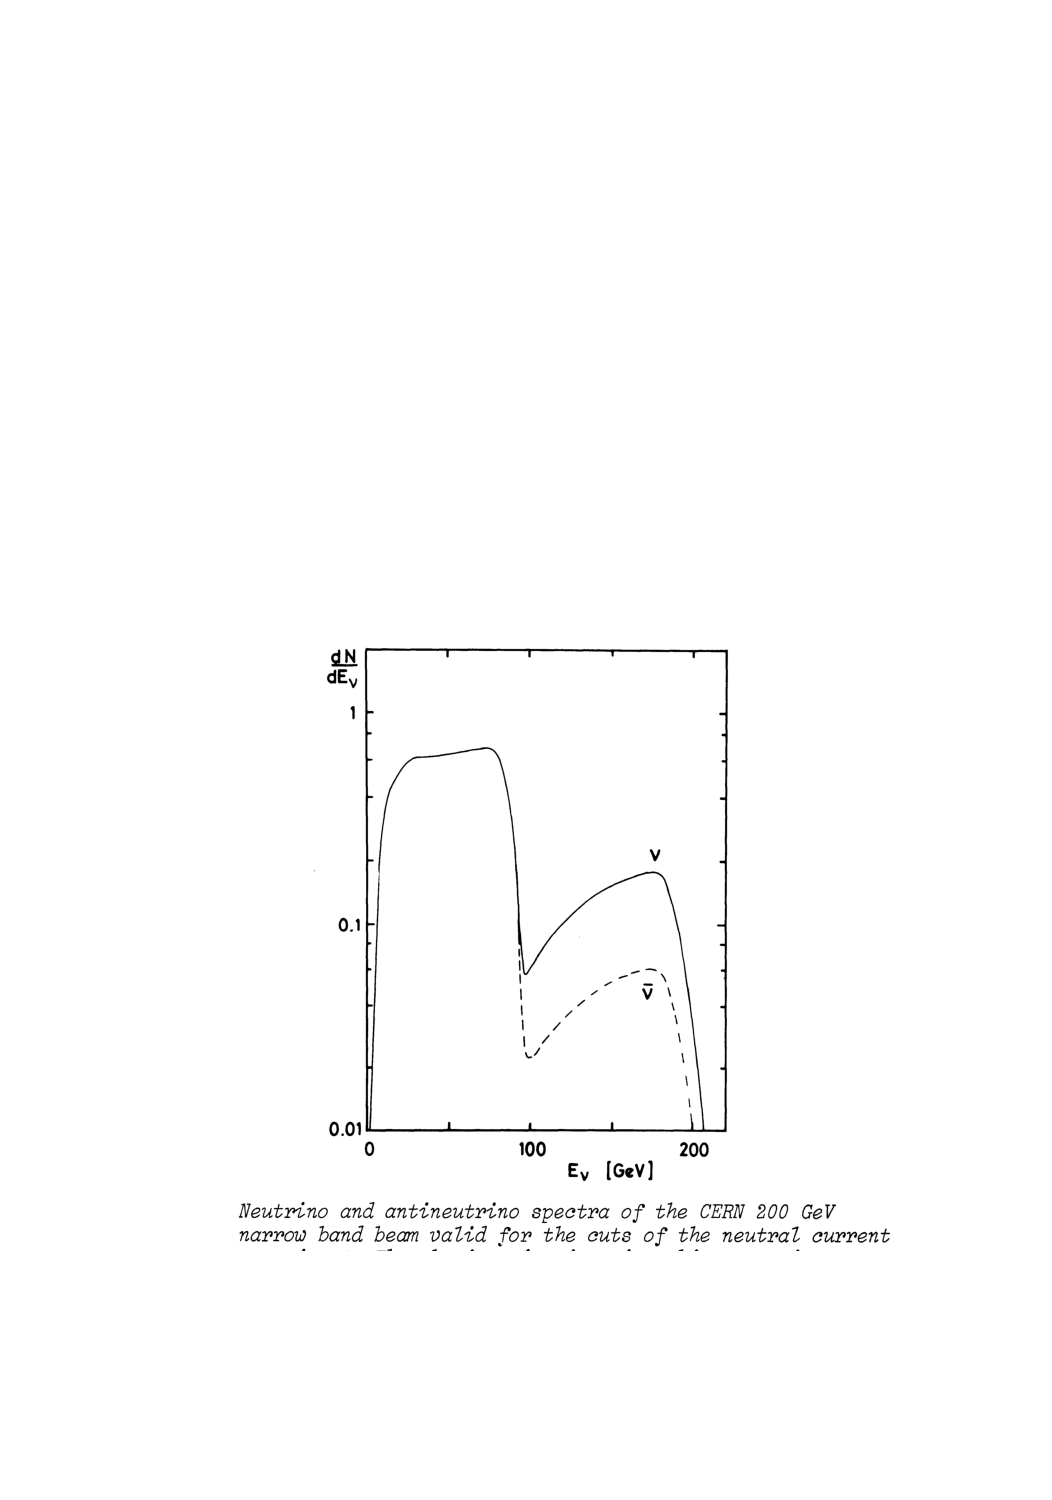
\includegraphics[height=0.65\textwidth]{./Images/CDHS04.pdf}
%   \end{center}
% \end{frame}  
% \end{document}


%\subsection{KARMEN experiment}
%%%%%% SLIDE
\begin{frame}{\textcolor{Goldenrod}{KARMEN experiment}}
  \hlt{SeaGreen}{The Karlsruhe Rutherford Medium Energy
    Neutrino(KARMEN) performed at the neutron spallation facility ISIS of
    the Rutherford Appleton Laboratory looking for:\\}
  \onslide<2->
  \[
    \begin{aligned}
      p + Ta-D_2O &\to \pi^+ + X \\
      &\qquad\pi^+ \to \mu^+ +\nu_{\mu}\\
      &\qquad\qquad\qquad\mu^+\to e^+ +\nu_e + \bar{\nu}_{\mu}\\
    \end{aligned}
  \]
  \itt
\item[$\Box$]<3-> \hlt{black}{Major physics aims:}
  \itt
\item<3-> the measurement of charged/neutral current (CC/NC)
\item<3-> neutrino-nucleon interactions
\item<3-> $\mu-e$ universality and the search for neutrino
  oscillations
  \tti
  \tti
\end{frame}

%%%%%%% SLIDE 
\begin{frame}{\textcolor{Goldenrod}{KARMEN: neutrino beam}}
  %% Cite https://arxiv.org/abs/1211.5199 
  \begin{figure}[h]
    \centering
    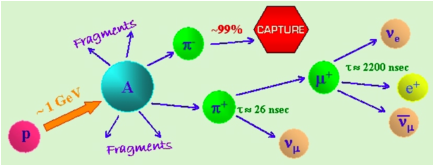
\includegraphics[height=0.25\textheight, width=0.8\linewidth]{./Images/KARMEN09}
  \end{figure}
  \itt  
\item[$\circ$] \hlt{BlueViolet}{The neutron spallation facility ISIS produced (by
    stopping $800 MeV$ protons in a beam dump $Ta-D_2O$ target) a
    $\nu$-source with identical intensities for all neutrino flavors
    emitted}
\item[$\circ$] \alert{Spallation refers to nuclear reactions that occurs when energetic
    hadrons (for example, protons, neutrons, or pions) hits a neuclus target}
\item[$\circ$]<2-> $\Phi_{\nu} = 6.37 \times 10^{13} \nu/s$ per flavor for
  $p$-beam current $I_p = 200 \mu A$
  \tti
  \note{$100 \mu A =  6.24 x 10^{14}$ protons per second
    striking the target.}
\end{frame}


%%%%%% SLIDE 
\begin{frame}{\textcolor{Goldenrod}{KARMEN: detector}}
\note{Due to the required good energy and time resultion and the extremely
  low cross section of the neutrino reactions}
\begin{overlayarea}{\textwidth}{\textheight}
 \begin{figure}[h]
    \centering
    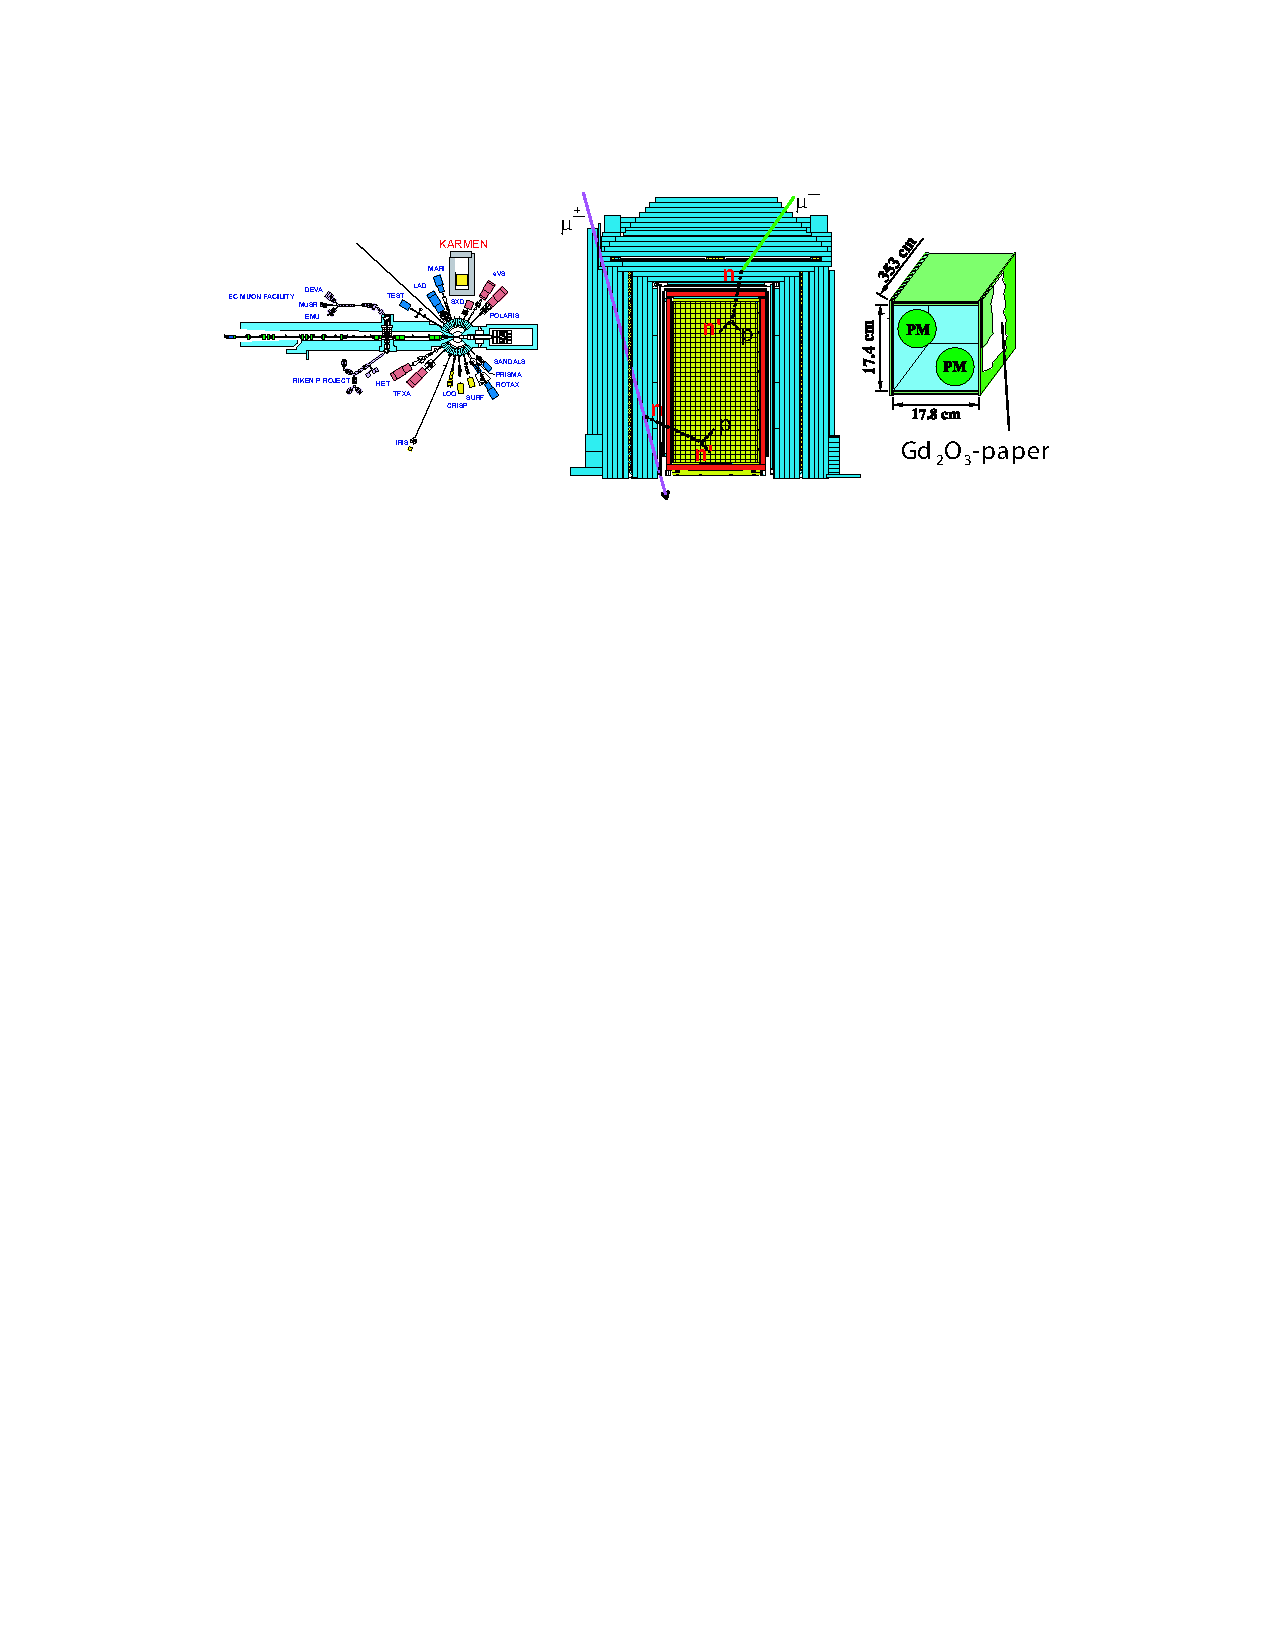
\includegraphics[height=0.4\textheight, width=0.9\linewidth]{./Images/KARMEN10}
  \end{figure}
\itt[<only@+>]
\item \hlt{Magenta}{The KARMEN-detector was
    constructed as a large volume liquid scintillation calorimeter.}
\item The central part of the detector consists of a $6 \times 3.53
  \times 3.20 m^3$ stainless steel tank($m = 7000 t$) filled with $65000 l$ of a
  dedicated liquid scintillator.
  \alert{The liquid scintillator is made of $75$\% vol. parrafin,
    $25$\% vol. pseudocumene}
  
  \note{A massive blockhouse of $7000 t$ of steel in combination with a system
    of two layers of active veto counters provides shielding against beam
    correlated spallation neutron background, suppression of the hadronic
    component of cosmic radiation as well as reduction of the flux of
    cosmic muons.}
  \note{pseudocumol and an admixture $2 g/l$ of the scintillator PMP
    (1-Phenyl-3-Mesityl-2-Pyrazolin).
    This mixture provides a very high
    lightoutput of $7.2 photons/keV$ and a attenuation length of $5 m$ at a
    wavelength of $425 nm$ wich perfectly fits to the dimensions of the
    detector.}
\item The central scintillation calorimeter and the inner veto
  counters are segmented by double acrylic walls with an air gap
  allowing efficient light transport via total internal reflection of
  the scintillation light at the module walls.
\item \hlt{BurntOrange}{The event position is
    determined by the individual module and the time difference of the PM
    signals at each end of this module.}
  \tti
\end{overlayarea}  
\end{frame}


%%%%%%% SLIDE
\begin{frame}{\textcolor{Goldenrod}{KARMEN: $\bar{\nu}_{\mu}\leftrightarrow
      \bar{\nu}_e$ search results}}
  \begin{figure}[h]
    \centering
    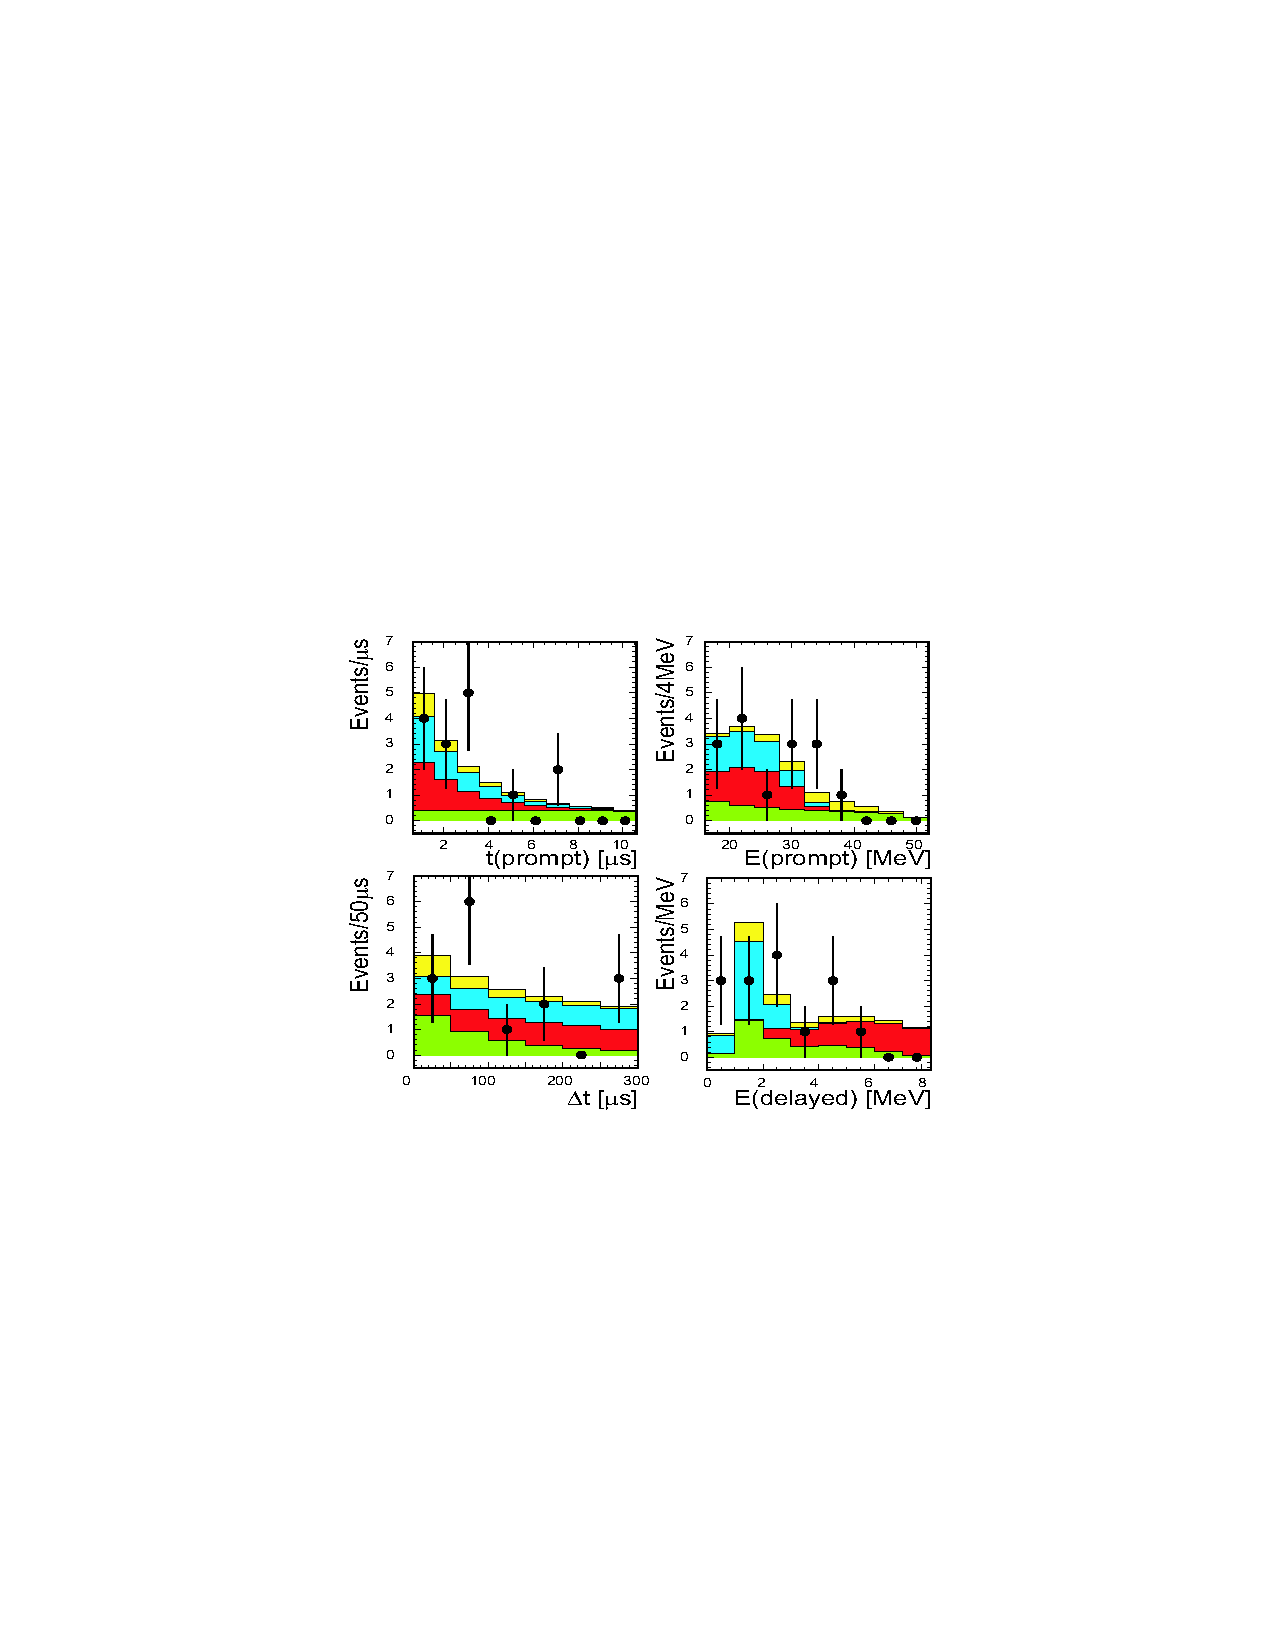
\includegraphics[height=0.4\textheight, width=0.6\linewidth]{./Images/KARMEN11}
    \caption*{KARMEN 15 coincidence candidates after final cuts}
  \end{figure}
\itt
\item $\sum_{bkg} = 15.8 \pm 0.5 events$
\item \hlt{Red}{extracted number of sequences is in excellent agreement with the
  background expectation, consistent with no additional $\bar{\nu}_e$ signal}
\tti  
\end{frame}


%\subsection{DONUT experiment}
%%%%%% SLIDE
\begin{frame}{\textcolor{Goldenrod}{DONUT experiment}}
  %% \cite A first measurement of the interaction cross section of the tau neutrino
  \hlt{Magenta}{The tau neutrino, $nu_{\tau}$, was added to the Standard Model
    after $\tau$ lepton discovery in 1975.}
  \itt
\item<2-> The difficulty of measuring $\nu_{\tau}$
  interactions was due to the relative scarcity of the sources of $\nu_{\tau}$ and
  the lack of sufficiently powerful detection methods to unambiguously
  identify the short-lived $\tau$ lepton.
  
\item<3-> Direct Observation of Nu-Tau (DONuT) experiment was designed to
  overcome these challenges
  \[
    \begin{aligned}
      &\nu_{\tau} + N \to \tau + X (SIG)\\
      & \nu_{e,\mu} + N \to e/\mu +  [D/D_s/\Lambda] + X (BKG 1)\\
      & \nu_l + N \to \nu_l + h^{\pm} ; h^{\pm}  + X \to \tau_{fake} +
      X^0 (BKG 2)\\
    \end{aligned}
  \]
  \tti    
\end{frame}

%%%%%% SLIDE
\begin{frame}{\textcolor{Goldenrod}{DONUT experiment: neutrino beam}}
  \begin{overlayarea}{\textwidth}{\textheight}
    \begin{figure}[h]
      \centering
      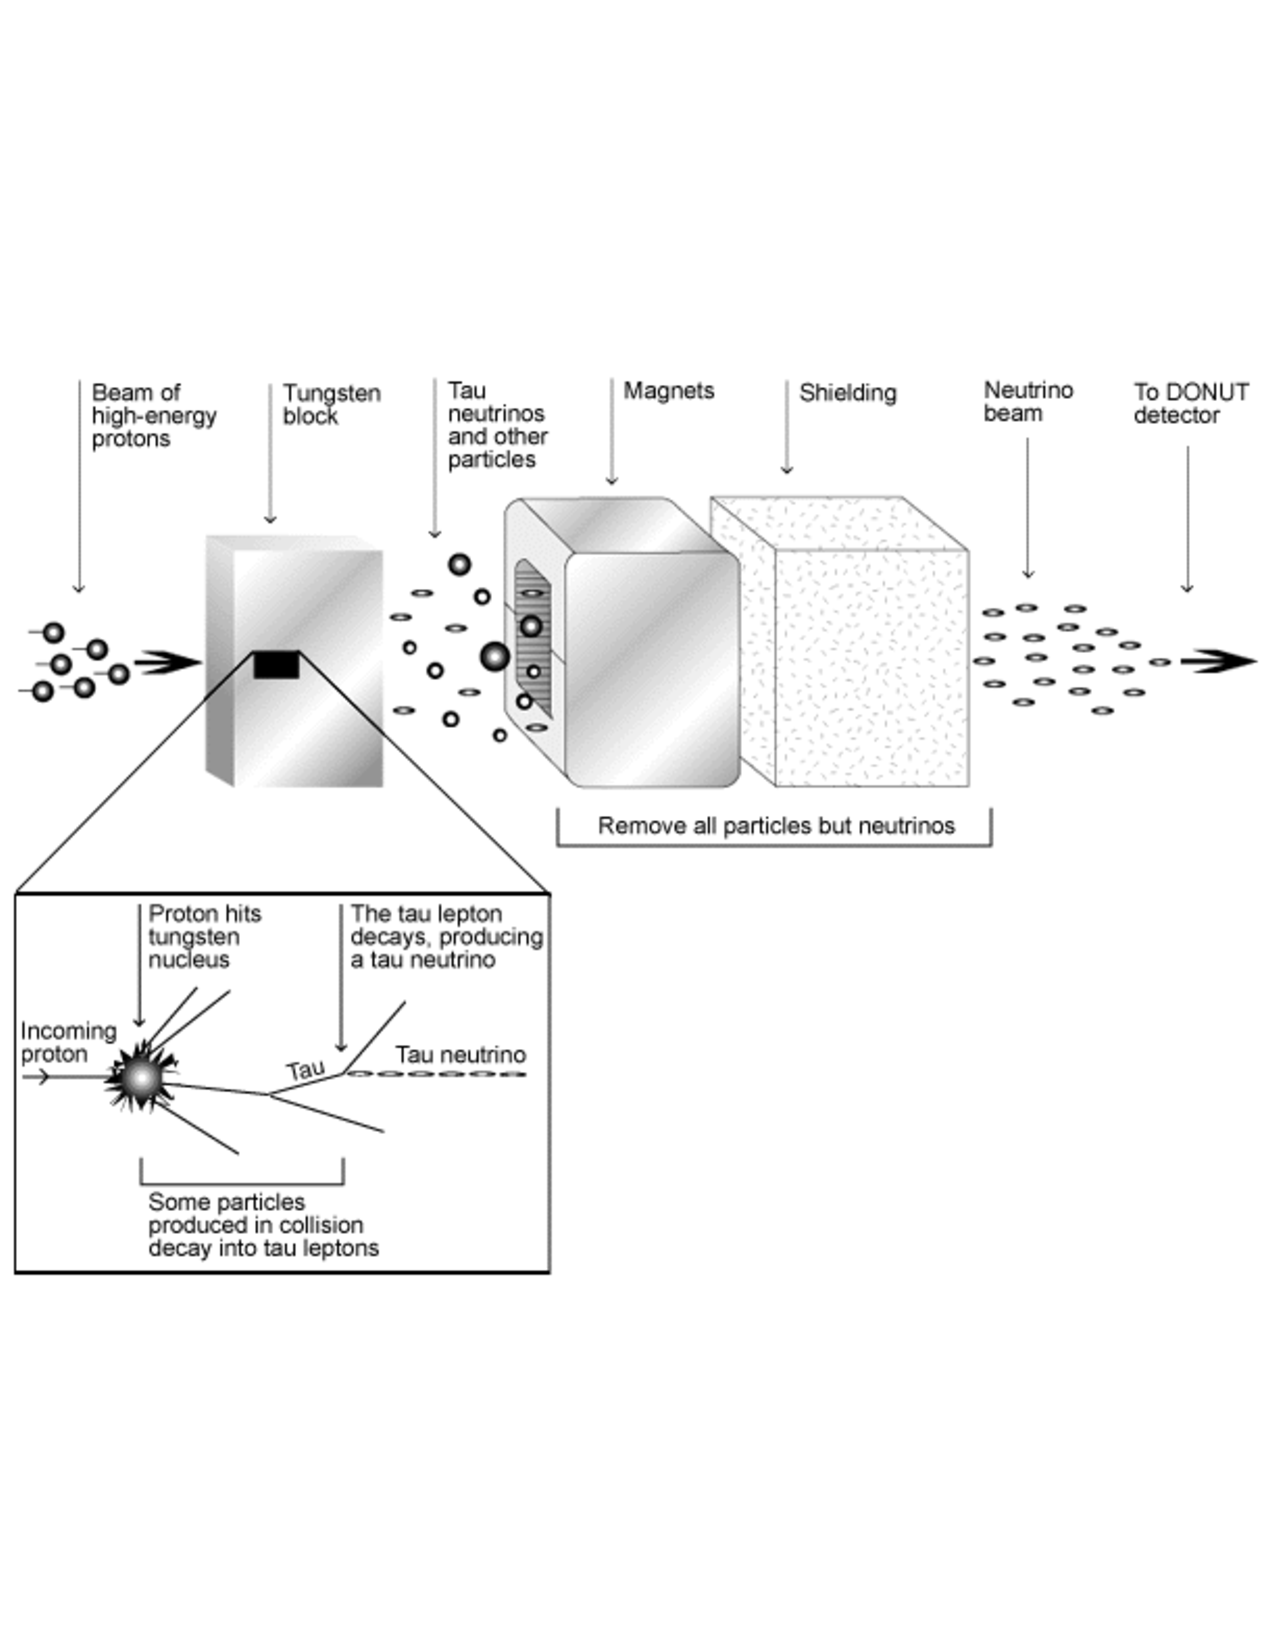
\includegraphics[height=0.4\textheight, width=0.6\linewidth]{./Images/DONUT02}
    \end{figure}
    
    \itt[<only@+>]
  \item The $800 GeV$ protons from the Tevatron were stopped in a
    beamdump in the form of a solid block of tungsten alloy. The
    typical intensity was $8 \times 10^{12}$ protons for $20$ seconds each minute
  \item Neutrinos in the DONuT beam originated from decays of
    particles within the hadron shower created by a primary proton
    interaction.
    \note{Neutrinos from decays of charmed particles are called
      prompt neutrinos, and neutrinos from decays of $\pi$ and $K$ are called
      non-prompt neutrinos.}
  \item \hlt{Red}{only $3$\% of the neutrino flux is $\nu_{\tau}$ and most of them originated
      in leptonic decays of $D_s \to \tau \nu_{tau}$}
    \note{yielded two tau
      neutrinos within a distance of a few
      millimeters. This decay length is
      much less than the interaction length
      of six centimeters.}
    \tti
  \end{overlayarea}
\end{frame}

%%%%%% SLIDE
\begin{frame}{\textcolor{Goldenrod}{DONUT experiment: detector}}
    \begin{overlayarea}{\textwidth}{\textheight}
    \begin{figure}[h]
      \centering
      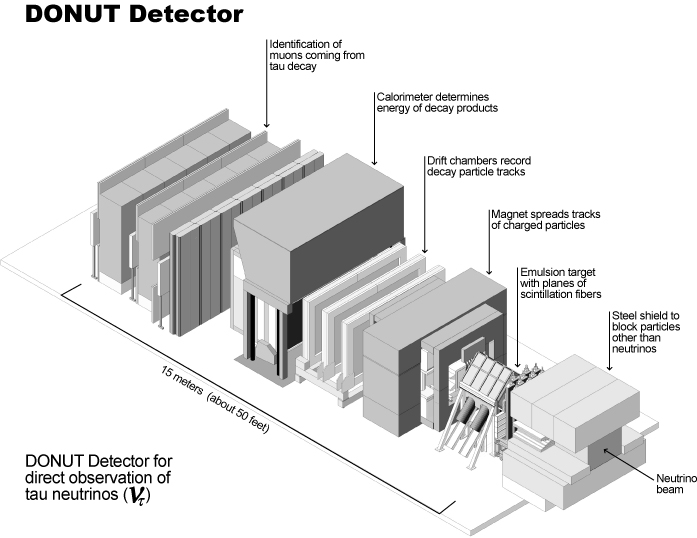
\includegraphics[height=0.45\textheight]{./Images/DONUT01}
    \end{figure}
    
  \note{The spectrometer was located 36 meters downstream of the proton beam
  target. Its main purpose included the identification of neutrino
  interactions, the measurement of event parameters, and the prediction
  of the neutrino interaction vertex location in the emulsion.

  Neutrino interactions were selected by the trigger system, which
  required the production of several high-momentum particles in the
  spectrometer with no incoming charged particle track.
  
  Event parameters were determined by three detector elements: the
  electromagnetic calo- rimeter was used to identify electron-neutrino
  interactions and to measure the electromag- netic energy, the muon ID
  system was used to identify muons produced in the neutrino
  interaction, and a combination of drift chambers and a magnetic field
  was used to measure the momentum of charged particles produced in the
  interaction.
  
  Scanning all of the emulsion volume with the current setup would take
  100 years , and the scanning time is proportional to the scan
  volume. To reduce the amount of emulsion that had to be scanned, the
  vertex location was estimated with the spectrometer to within about
  2mm from reconstructed charged particle tracks.}

\itt[<only@+>]
\item[$\Box$] \hlt{black}{The Trigger Counters:}\\
  {\small At least two high-momentum charged particle tracks coming
  from the emulsion targets and no incoming charged particles.\\
  Charged particles entering the upstream side were rejected by the veto
  wall.}
  \note{It consisted of two planes of $2.64 m\times 0.35m\times 1.93m$
  scintillator counters and each plane contained five counters.
  Photomultiplier tubes (PMT) mounted at both ends of the counters
  converted light from the scintillators into electronic signals.
  Each of the counters had a detection efficiency for minimum ionizing
  particles of better than 95\%, which gives a veto wall efficiency of
  better than 99\%.}
\item[$\Box$] \hlt{black}{The Scintillating Fiber Tracking System:}\\
  The scintillating fiber planes provided position measurements
  for several sampling points along the track.
  \note{A scintillating fiber detector was used to predict the position of the
    neutrino interaction vertex in the emulsion by recording the
    high-momentum charged particle tracks coming from the interaction
    vertex.}
  \note{The fiber planes
  were interleaved with the emulsion modules to provide at least four
  sampling points in two different orientations for each charged
  particle track.}

\item[$\Box$] \hlt{black}{Downstream Tracking:}\\
  {\small Charged particle tracks coming from the neutrino interaction vertex
  and identified in the scintillating fiber system give information
  about the neutrino interaction parameters. \alert{The particle momentum for
  these tracks was determined through the combination of drift cham- ber
  tracking and deflection in a magnetic field}}

\item[$\Box$] \hlt{black}{The Electromagnetic Calorimeter:}\\
  {\small tau decays produce
    high-energy electrons. As they pass through material, these
    electrons generate electromagnetic showers that can be identified in
    the electromagnetic calorimeter (EMCAL), which provided an estimate
    for the electromagnetic energy of individual particles.}

  \note{The EMCAL was segmented into $400$ lead glass and scintillating glass
  blocks of dimension $0.15m \times 0.15m \times 0.89m$.}

\item[$\Box$]  \hlt{black}{Muon Identification:}\\
  A muon neutrino charged-current interaction can be uniquely identified
  by the muon produced in the interaction.\\
  \note{Unlike electrons and
    hadrons, muons can pass through a lot of material, they only lose
    energy through ionization, whereas electrons lose their energy in
    electromagnetic showers and hadrons lose their energy in hadronic
    showers.}
  
  \note{A three-layer sandwich of steel plates and detectors was used to
    identify muons downstream of the electromagnetic calorimeter. The
    steel stopped electrons and hadrons, only muons passed through to
    produce hits in the active detector planes}
  \tti
\end{overlayarea}
\end{frame}

%%%%%% SLIDE
\begin{frame}{\textcolor{Goldenrod}{DONUT experiment}}
  \begin{overlayarea}{\textwidth}{\textheight}
    \begin{figure}[h]
      \centering
      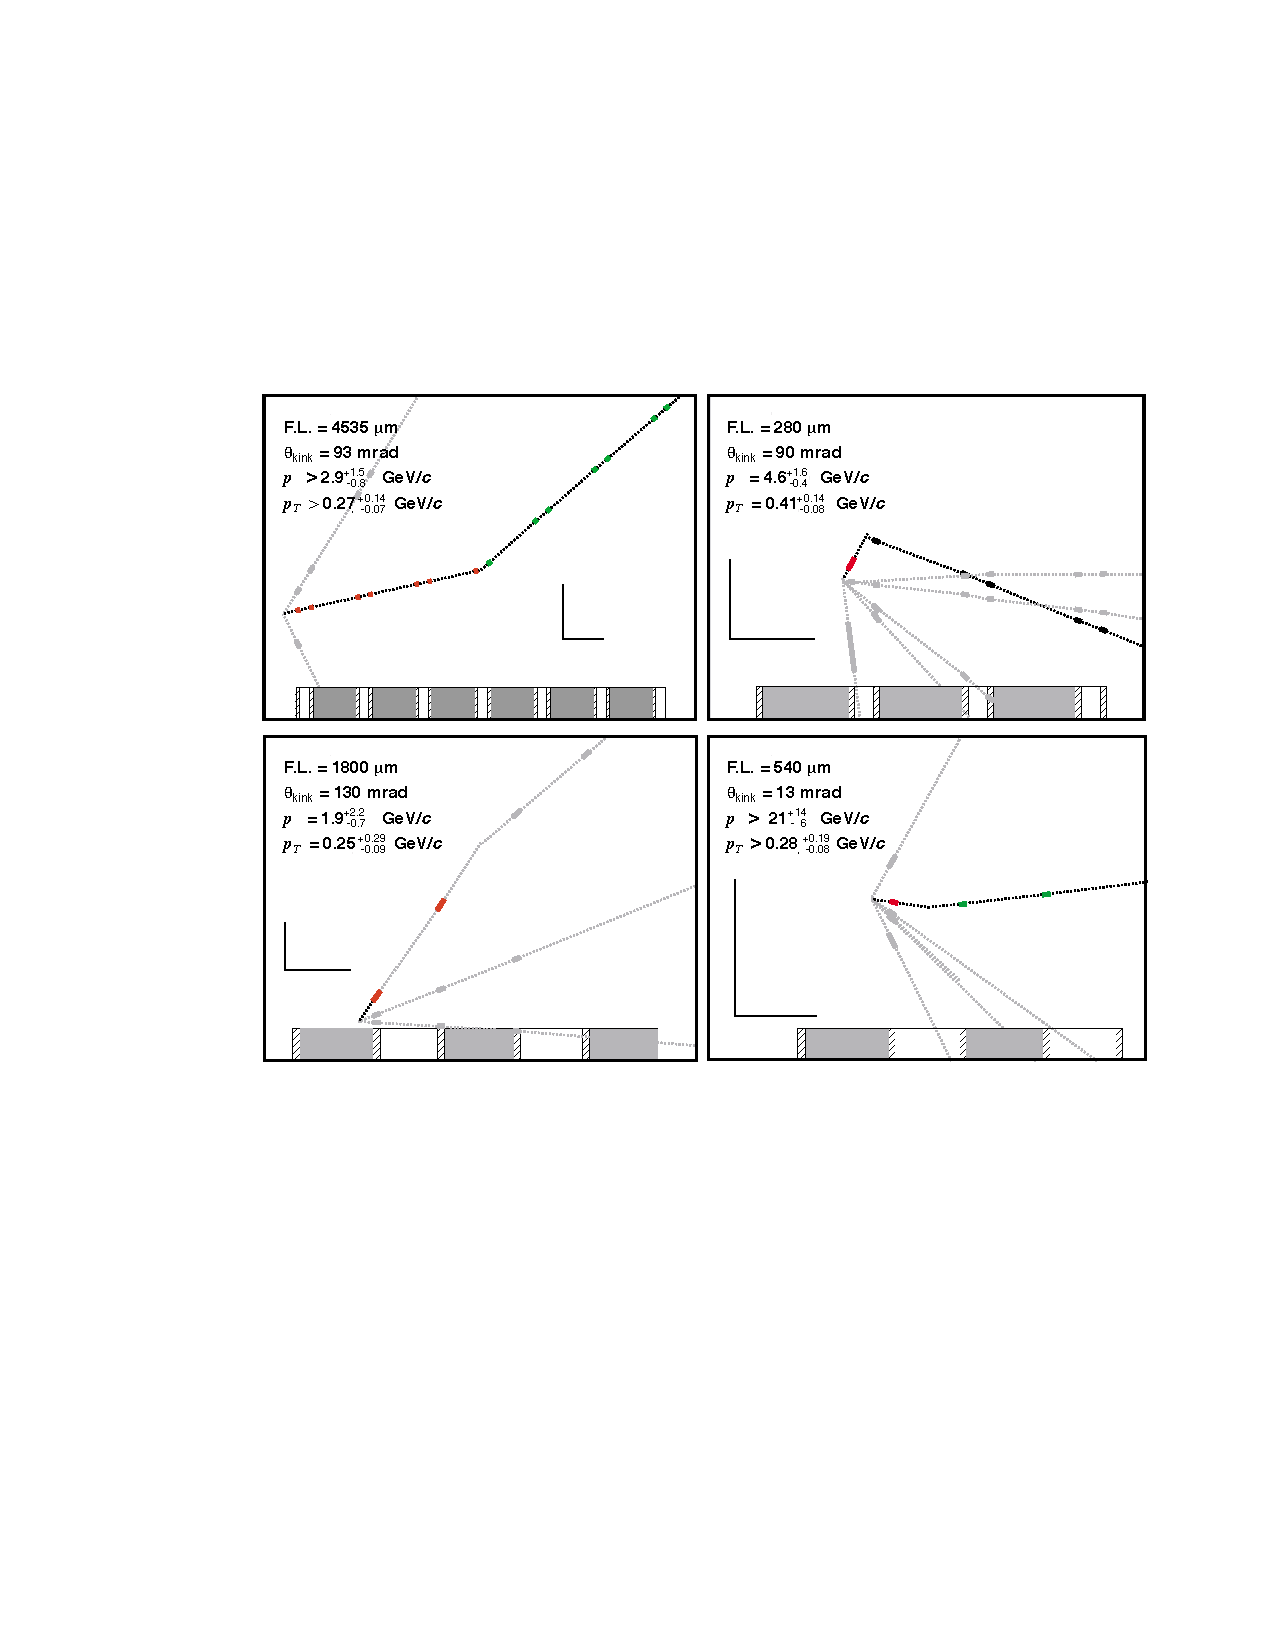
\includegraphics[height=0.4\textheight]{./Images/DONUT03}
    \end{figure}
    
    \itt[<only@+>]
  \item The four $\nu_{\tau}$ CC interaction events. The scale is
given by the perpendicular lines with the vertical line representing
$0.1mm$ and the horizontal $1mm$. {\small The target material is shown
by the bar at the bottom of each part of the figure representing steel
(shaded), emulsion (cross hatched) and plastic (no shading)}
  \item out of $203$ located neutrino interactions four events have a
track that meets all the requirements for $\tau$ decays . The total
background is estimated to b e $\sum_{bkg} = 0.34 \pm 0.05$ \to $> 4
\sigma $ \to discovery
    
    \note{The
      probability that the four events are from background sources is
      $4\times 10^{-4}$. We conclude that these events are evidence that
      $\tau$ CC interaction has been observed.}
    \tti
  \end{overlayarea}
\end{frame}





\backupend
\end{document}
